% !TEX root = ../main.tex

\chapter{Machine learning state of the art} \label{chap:state-of-the-art}

\begin{displayquote}
	\textit{This chapter starts defining the concept of machine learning in its two major declinations: supervised and unsupervised learning. It continues providing a comprehensive overview  of algorithms, models and techniques relevant for the biomedical data science applications described in Part II. At the end of this chapter, an overview on the computational requirements and the most recent machine learning technologies is given.}
\end{displayquote}

The term \textit{Machine Learning} (ML) first appeared in the late 50's in the field of computer science and it is now becoming a buzzword used in several contexts spanning from particle physics and astronomy to medicine and social sciences~\cite{service2017ai}.
With a simple search on Google Trends\footnote{\url{https://trends.google.com}} it is possible to roughly quantify the pervasiveness of this term on the Internet in the last few years. From Figure~\ref{fig:google_trend_ML} we can see that the interest toward both the terms \textit{machine learning} and \textit{data science} is growing, with the first consistently superior to the second.

\begin{figure}[h!]
  \centering
    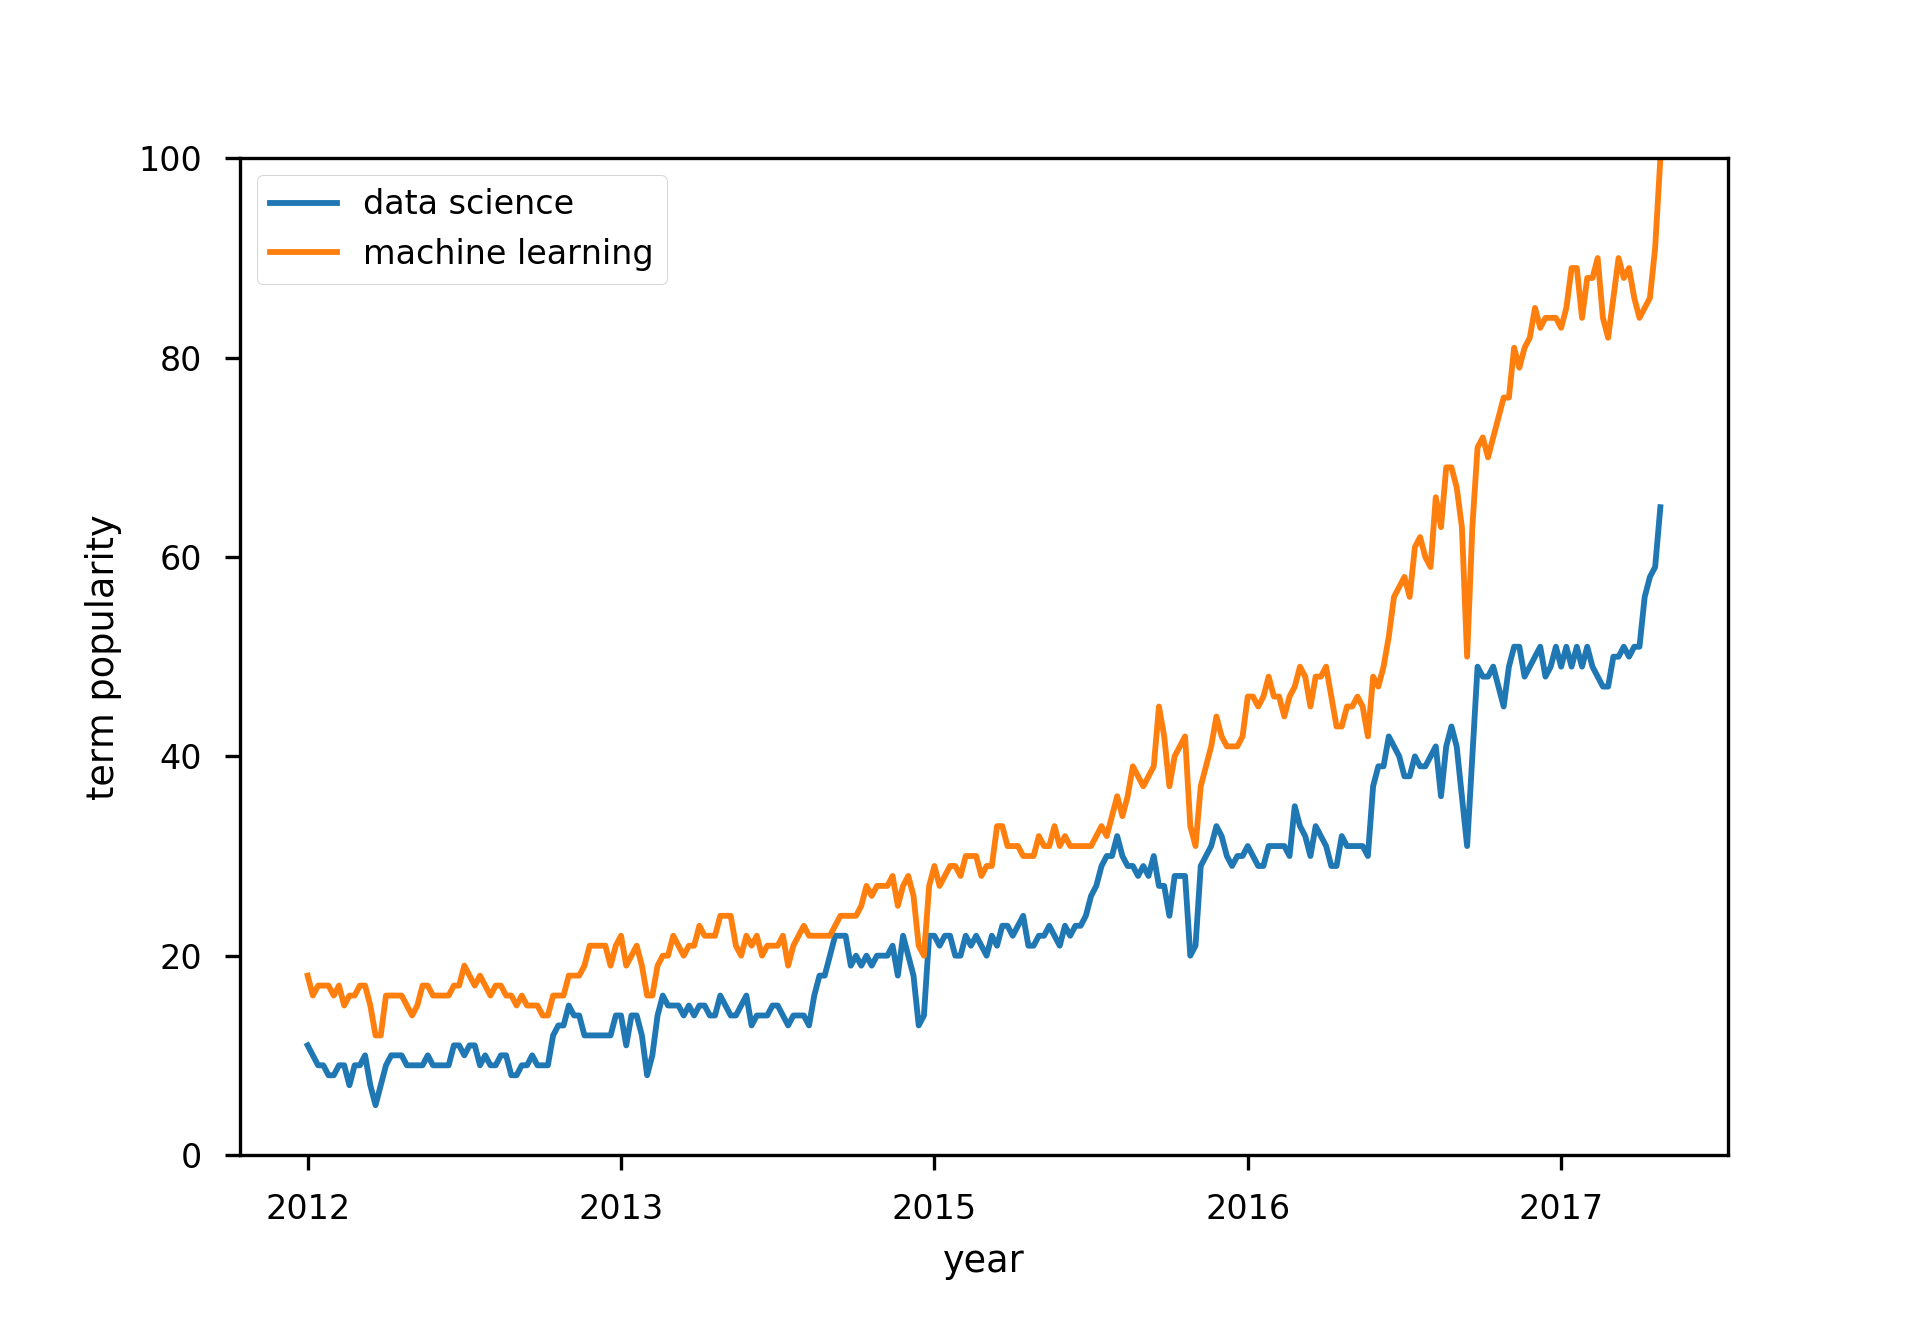
\includegraphics[width=0.8\textwidth]{part1/google_trends_MLDS.png}
  \caption{The Internet popularity over the past five years of two terms: \textit{data science} and \textit{machine learning}. The vertical axis represents the number of Google searches of an input term normalized with respect to its maximum (source: Google Trends).} \label{fig:google_trend_ML}
\end{figure}

A partial explanation to this phenomenon can be found in a recent article published on Science~\cite{appenzeller2017revolution}, where the authors observed how the explosion of modern data collection abilities is leading the human kind toward another \textit{scientific revolution}.
Biomedical applications are prototypical in this sense. For instance, the volume of the raw data acquired from a genome sequencer for a single \ac{DNA} has a volume of approximately 140 GB~\cite{marx2013biology}. Another example can be the 3D reconstruction of cardiac MRI acquisition which needs around 20 GB for a single human heart, or the 3D \ac{CT} scan which has a volume in the order of GB for each patient, and so on. It has been estimated that an average hospital currently stores more than 665 TB of data that needs to be analyzed and understood.
%the typical resolution of MRI images is currently $512 \times 512$
Such massive amounts of data have long overwhelmed human analysis and insights potential. This makes ML a key element for clinicians and scientists that try to make sense of large-scale observations.

But, what is \textit{machine learning}? And how does it differ from classical statistics?

A unique answer to this question is not easy to provide. In fact, ML can be defined in different ways and from several standpoints. Let's see three remarkable examples.

\begin{enumerate}
  \item Kevin P. Murphy in its \emph{Machine Learning - A Probabilistic Perspective}~\cite{murphy2012machine} defines machine learning as follows.

  \begin{displayquote}
  "$[\dots]$ \emph{a set of methods that can automatically detect patterns in data, and then use the uncovered patterns to predict future data, or to perform other kinds of decision making under uncertainty} $[\dots]$"
  \end{displayquote}

  \item Trevor Hastie, a well-known applied statistician, in a famous seminar\footnote{part of Data Science @ Stanford Seminar series (source: \url{https://goo.gl/UFgqxU})}, held in October 2015 at the Stanford University, gave the following three definitions.

  \begin{displayquote}
    \begin{itemize}
      \item[] \emph{{\bf Machine Learning} constructs algorithms that can learn from data.}
      \item[] \emph{{\bf Statistical Learning}  is a branch of applied statistics that emerged in response to machine learning, emphasizing statistical models and assessment of uncertainty.}
      \item[] \emph{{\bf Data Science}  is the extraction of knowledge from data, using ideas from mathematics, statistics, machine learning, computer science, engineering...}
    \end{itemize}
  \end{displayquote}

  \item Carl E. Rasmussen in the preface of its renowned \emph{Gaussian Processes for Machine Learning}~\cite{rasmussen2006gaussian} introduces the difference between classical statistics and ML as follows.

  \begin{displayquote}
    "$[\dots]$ \emph{in statistics a prime focus is often in understanding the data and relationships in terms of models giving approximate summaries such as linear relations or independencies. In contrast, the goals in machine learning are primarily to make predictions as accurately as possible and to understand the behaviour of learning algorithms} $[\dots]$"
  \end{displayquote}

\end{enumerate}

It looks like each author, according to his background, expertise and experience, provides a slightly different definition of ML. Trying to summarize these three standpoints, we can say that \emph{ML is an interdisciplinary field that borrows the concept of data-driven model from statistics in order to devise algorithms that can exploit hidden patterns in current data and make accurate predictions on future data}.

As of today ML is the workhorse of data science.


  \section{Supervised learning} \label{subsec:supervised_learning}

	  Humans are remarkably good at \emph{learning by examples}. When a kid is taught what a pencil looks like, he will be capable of understanding the concept of pencil from a limited number of guided observations. Similarly, when future radiologists are trained to distinguish between healthy tissues from tumors in MRI scans, they will be provided with several annotated biomedical images from which they will be able to generalize.
	  The applied learning paradigm is characterized by the presence of two key objects: \textit{data} and \textit{labels}. In the last example, the MRI scans are the data, and their annotations (\eg tumor \vs healthy tissue) are the labels.

	  Supervised learning is the branch of ML in which predictive models are trained on labeled data. In the ML jargon, and in this thesis, one usually refers to \textit{data} as collections of \textit{samples} described by an arbitrarily large number of \textit{predictors} (\textit{features}) that are used as \textit{input} in a training process having labels as \textit{output}.

	  Input samples throughout this thesis are represented as $d$-dimensional vectors $\bm{x}$ belonging to an input space $\mathcal{X}$, where typically $\mathcal{X}\subseteq\mathbb{R}^d$ and labels are represented with the variable $y$ belonging to an output space $\mathcal{Y}$.
	  The nature of $\mathcal{Y}$ defines the learning task as \textit{binary classification} if  $\mathcal{Y} = \{-1,+1\}$, \textit{multiclass classification} if $\mathcal{Y} = \{1,2,\dots,k\}$,
	  \textit{regression} if $\mathcal{Y}\subseteq\mathds{R}$ and
	  \textit{vector-valued regression} if $\mathcal{Y}\subseteq\mathds{R}^k$.
	%  In the second part of this thesis each of these learning problems will be faced.
	  The remainder of this section summarizes the methods that are most relevant with the data-driven strategies adopted to tackle the biomedical data science challenges described in the second part of in this thesis.

	  Given a set of input-output pairs $\mathcal{D} = \{\bm{x}_i, y_i\}_{i=1}^n = (X, \bm{y})$, supervised learning methods aim at finding a function of the inputs $f(\bm{x})$ that approximates the output $y$. This translates into the minimization problem defined in Equation~\eqref{eq:loss}.

	  \begin{equation}\label{eq:loss}
	    \argmin_{f \in \mathcal{F}} \frac{1}{n}\sum_{i=1}^n L(f(\bm{x}_i),y_i) %+ \lambda R(f)
	  \end{equation}

	  The loss function $L(f(\bm{x}),y)$ can be seen as a measure of \textit{adherence} to the available training data. Several loss functions for regression and classification problems were proposed; Table~\ref{tab:losses} defines the most commonly adopted in biomedical studies while their visual representation is presented in Figure~\ref{fig:loss}.
	  Choosing the appropriate loss function for the problem at hand is crucial and there is no trivial solution for this problem.
	  Different choices for $L(f(\bm{x}),y)$ identifies different learning machines, that are known under different names. The most popular methods will be presented in the next few sections.
	  % \todo{Different choices for the loss function imply different ML model, see the remainder of this section + this is possibly ill-posed}

	  \begin{table}[!h]
	  	\centering
	  	\caption{Definition of the loss functions for regression (top) and classification (bottom) problems represented in Figure~\ref{fig:loss}.}\label{tab:losses}
	  	\begin{tabular}{@{}ll@{}ll@{}}
	  		\toprule
	  		Loss function & $L(f(\bm{x}),y)$  & Learning problem           \\ \midrule
	  		Square                   & $(y - f(\bm{x}))^2$ & regression \\
	  		Absolute                 & $|y - f(\bm{x})|$ & regression   \\
	  		$\varepsilon$-insensitive   & $|y - f(\bm{x})|_\varepsilon$  & regression                 \\
	  		\midrule
	  		Zero-one               & $\mathds{1}\{y=f(\bm{x})\}$ & classification \\
	  		Square                 & $(1 - yf(\bm{x}))^2$ & classification  \\
	  		Logistic                 & $\log(1 + e^{-yf(\bm{x})})$ & classification  \\
	  		Hinge                 & $|1 - yf(\bm{x})|_+$ & classification  \\
	  		Exponential & $e^{- yf(\bm{x})}$ & classification \\
	  		\bottomrule
	  	\end{tabular}
	  \end{table}

	  \begin{figure}[!h]
	  	\centering
	  	\subfloat[]{%
	  		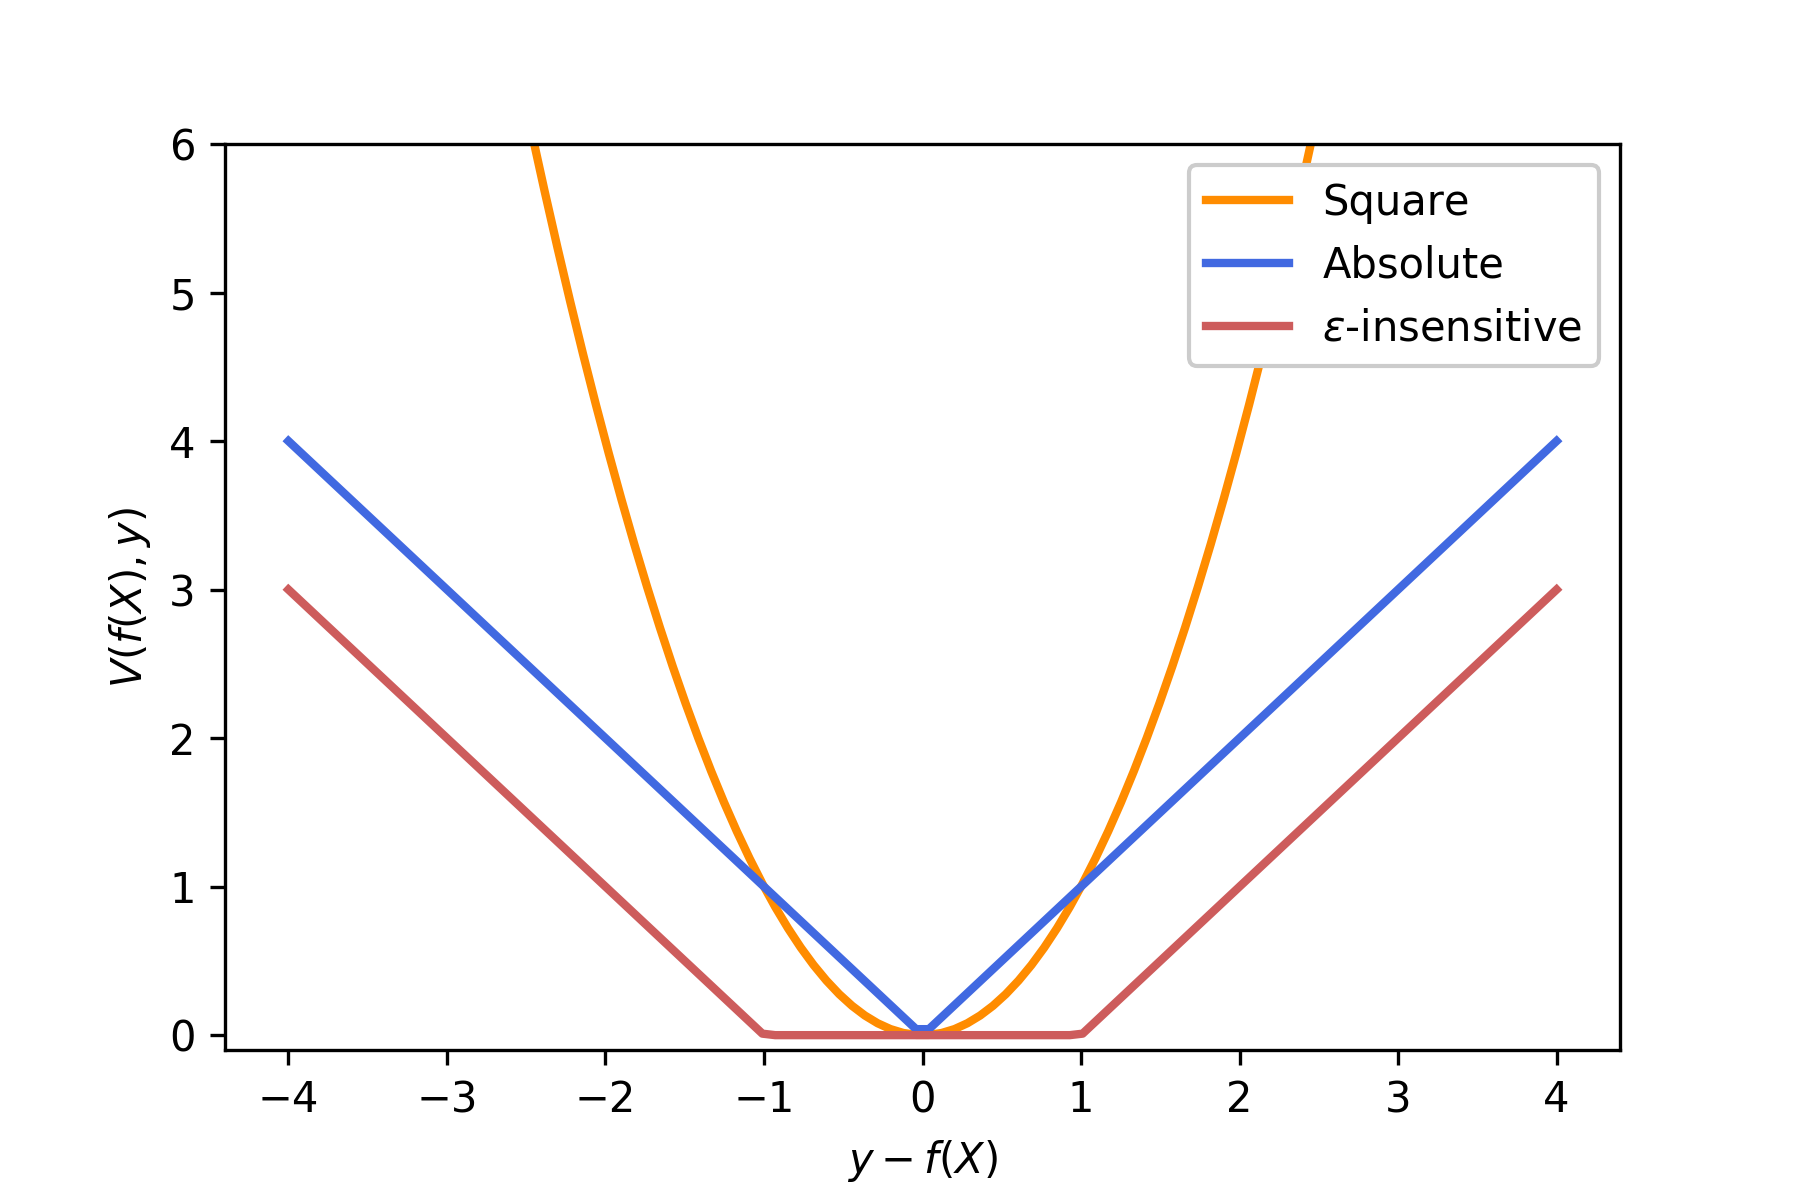
\includegraphics[width=0.5\textwidth]{part1/regression_losses.png}
	  		\label{fig:regression}%
	  	}%
	  	% \hfill%
	  	\subfloat[]{%
	  		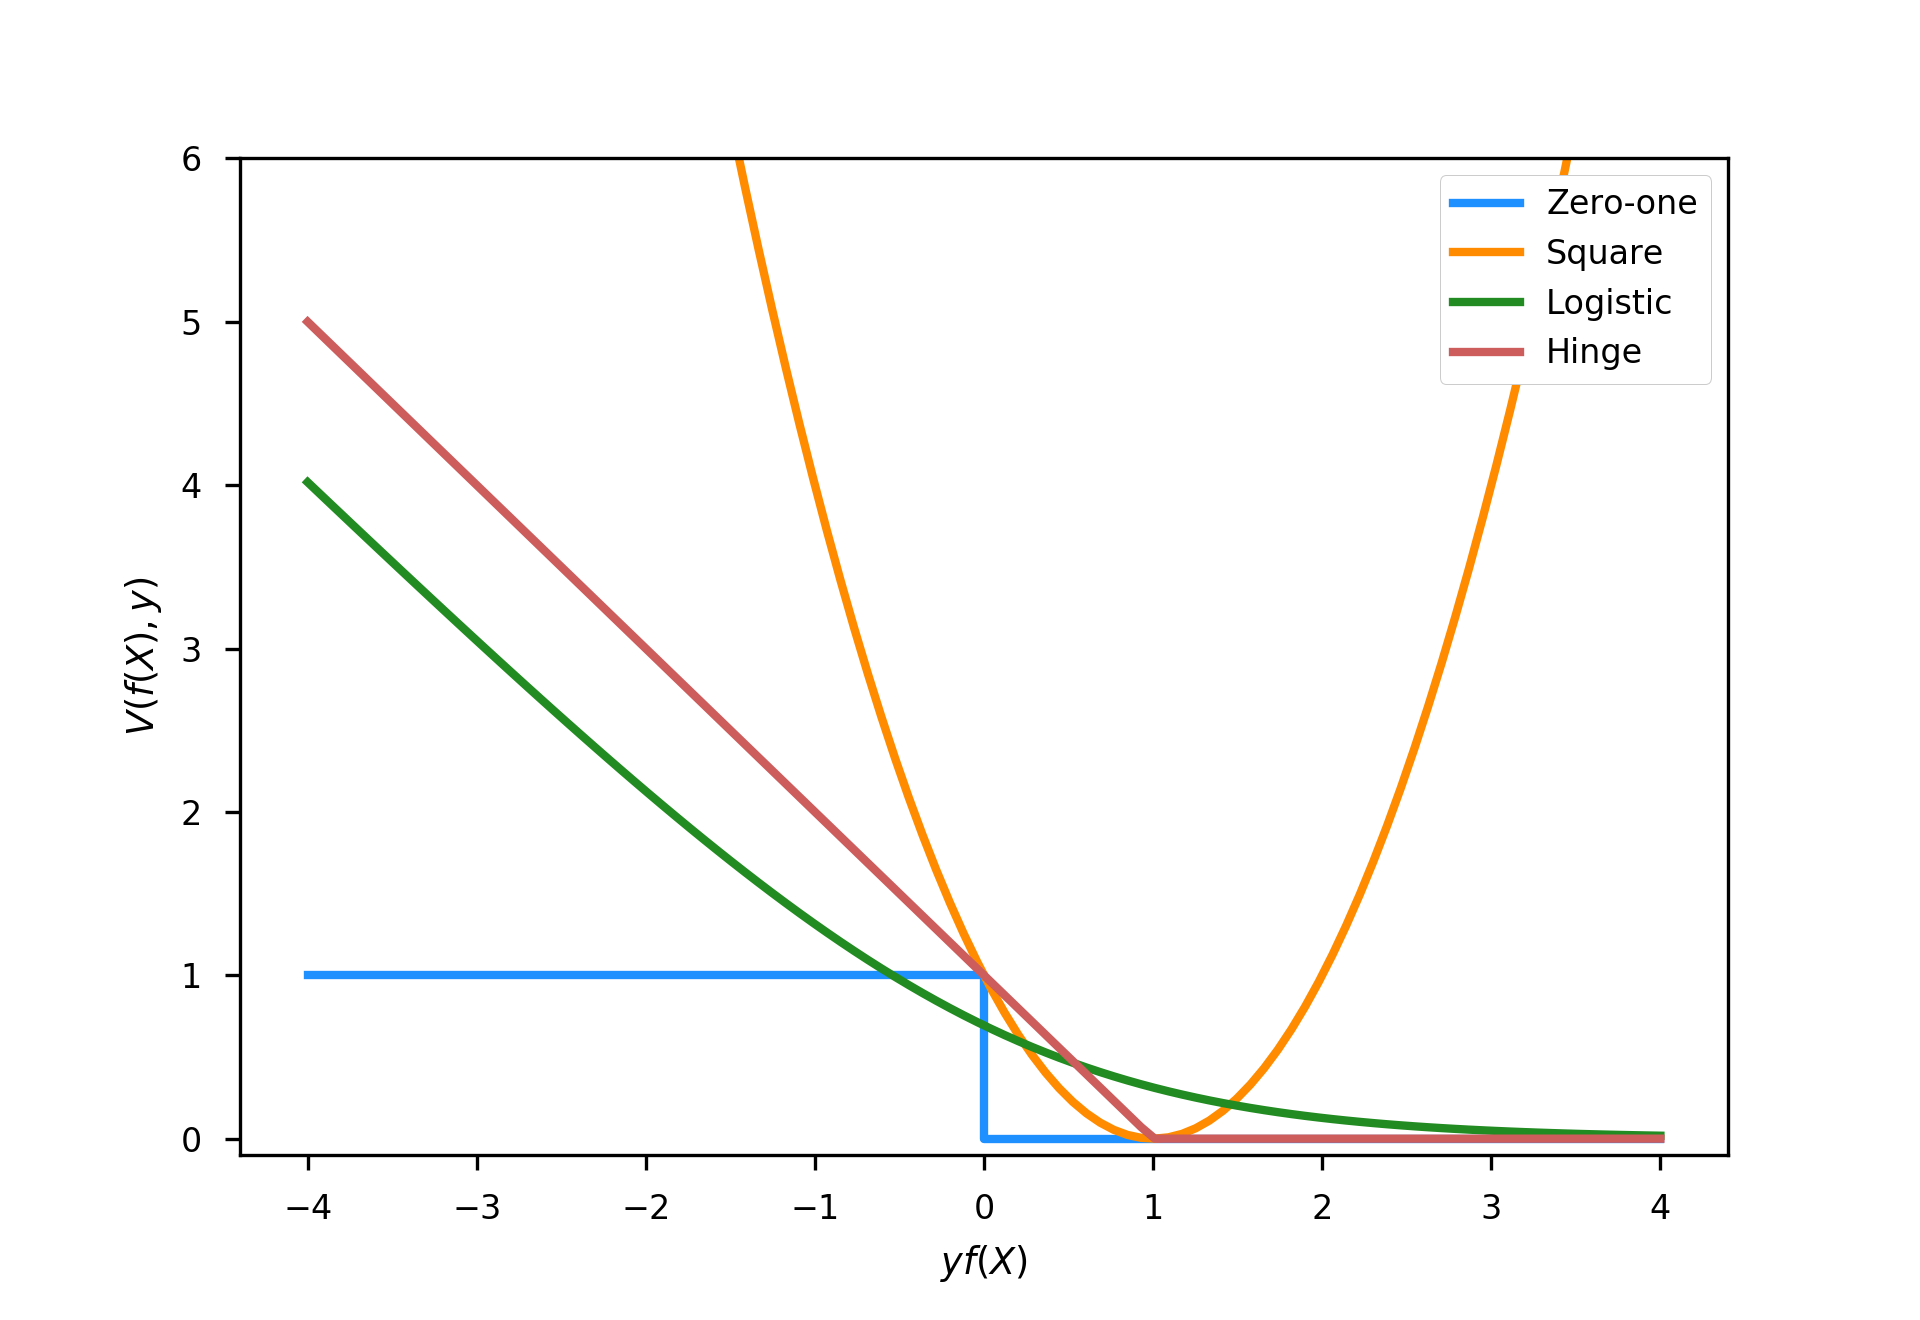
\includegraphics[width=0.5\textwidth]{part1/classification_losses.png} \label{fig:classification}
	  	}%
	  	\caption{An overview on the most common loss functions for regression (a) and classification (b) problems plotted against the corresponding prediction error.}\label{fig:loss}
	  \end{figure}

	   % rubare da BIB
	  % In its most classical definition, the aim of modeling is to infer some unknown structure underlying the data.
	  Identifying a reliable data-driven model can be a very tricky task. Many unwanted and concurrent factors may be misleading and the solution may have poor predictive power for several reasons.
		Including:
		\begin{enumerate}
			\item the acquisition devices may introduce random fluctuations in the measures;
			\item the amount of collected samples $n$ may be small with respect to the number of observed variables $d$;
			\item a non-negligible number of the measured variables may not be representative of the target phenomenon.
	  \end{enumerate}
		From a modeling standpoint, every combination of the factors above can be seen as \textit{noise} affecting the data.
		Precautions in the model formulation process must be taken in order to achieve solutions that are insensitive to small changes in the input data and that are, in general, \textit{robust} to the noise effect.

		Considering a ML model ($\hat f$) fitted on a collection of data ($\mathcal{D}$), the most desirable property of $\hat f$ is that it should be able to achieve good prediction performance not only on $\mathcal{D}$, but also on all the future, therefore unseen, data points $\mathcal{D}'$.
		In other words, assuming that the samples in $\mathcal{D}$ are affected by some kind of random\footnote{here with \textit{random} means "\textit{uncorrelated with the input-output relationship}"} component, $\hat f$ should be a predictive function that does not \textit{follow the noise}, but rather models the true input-output relationship.
		In ML, a model that fits well $\mathcal{D}$ but performs poorly on $\mathcal{D}'$ is said to be \textit{overfitting}.

	  \begin{figure}[!h]
	  	\centering
	  	\subfloat[]{%
	  		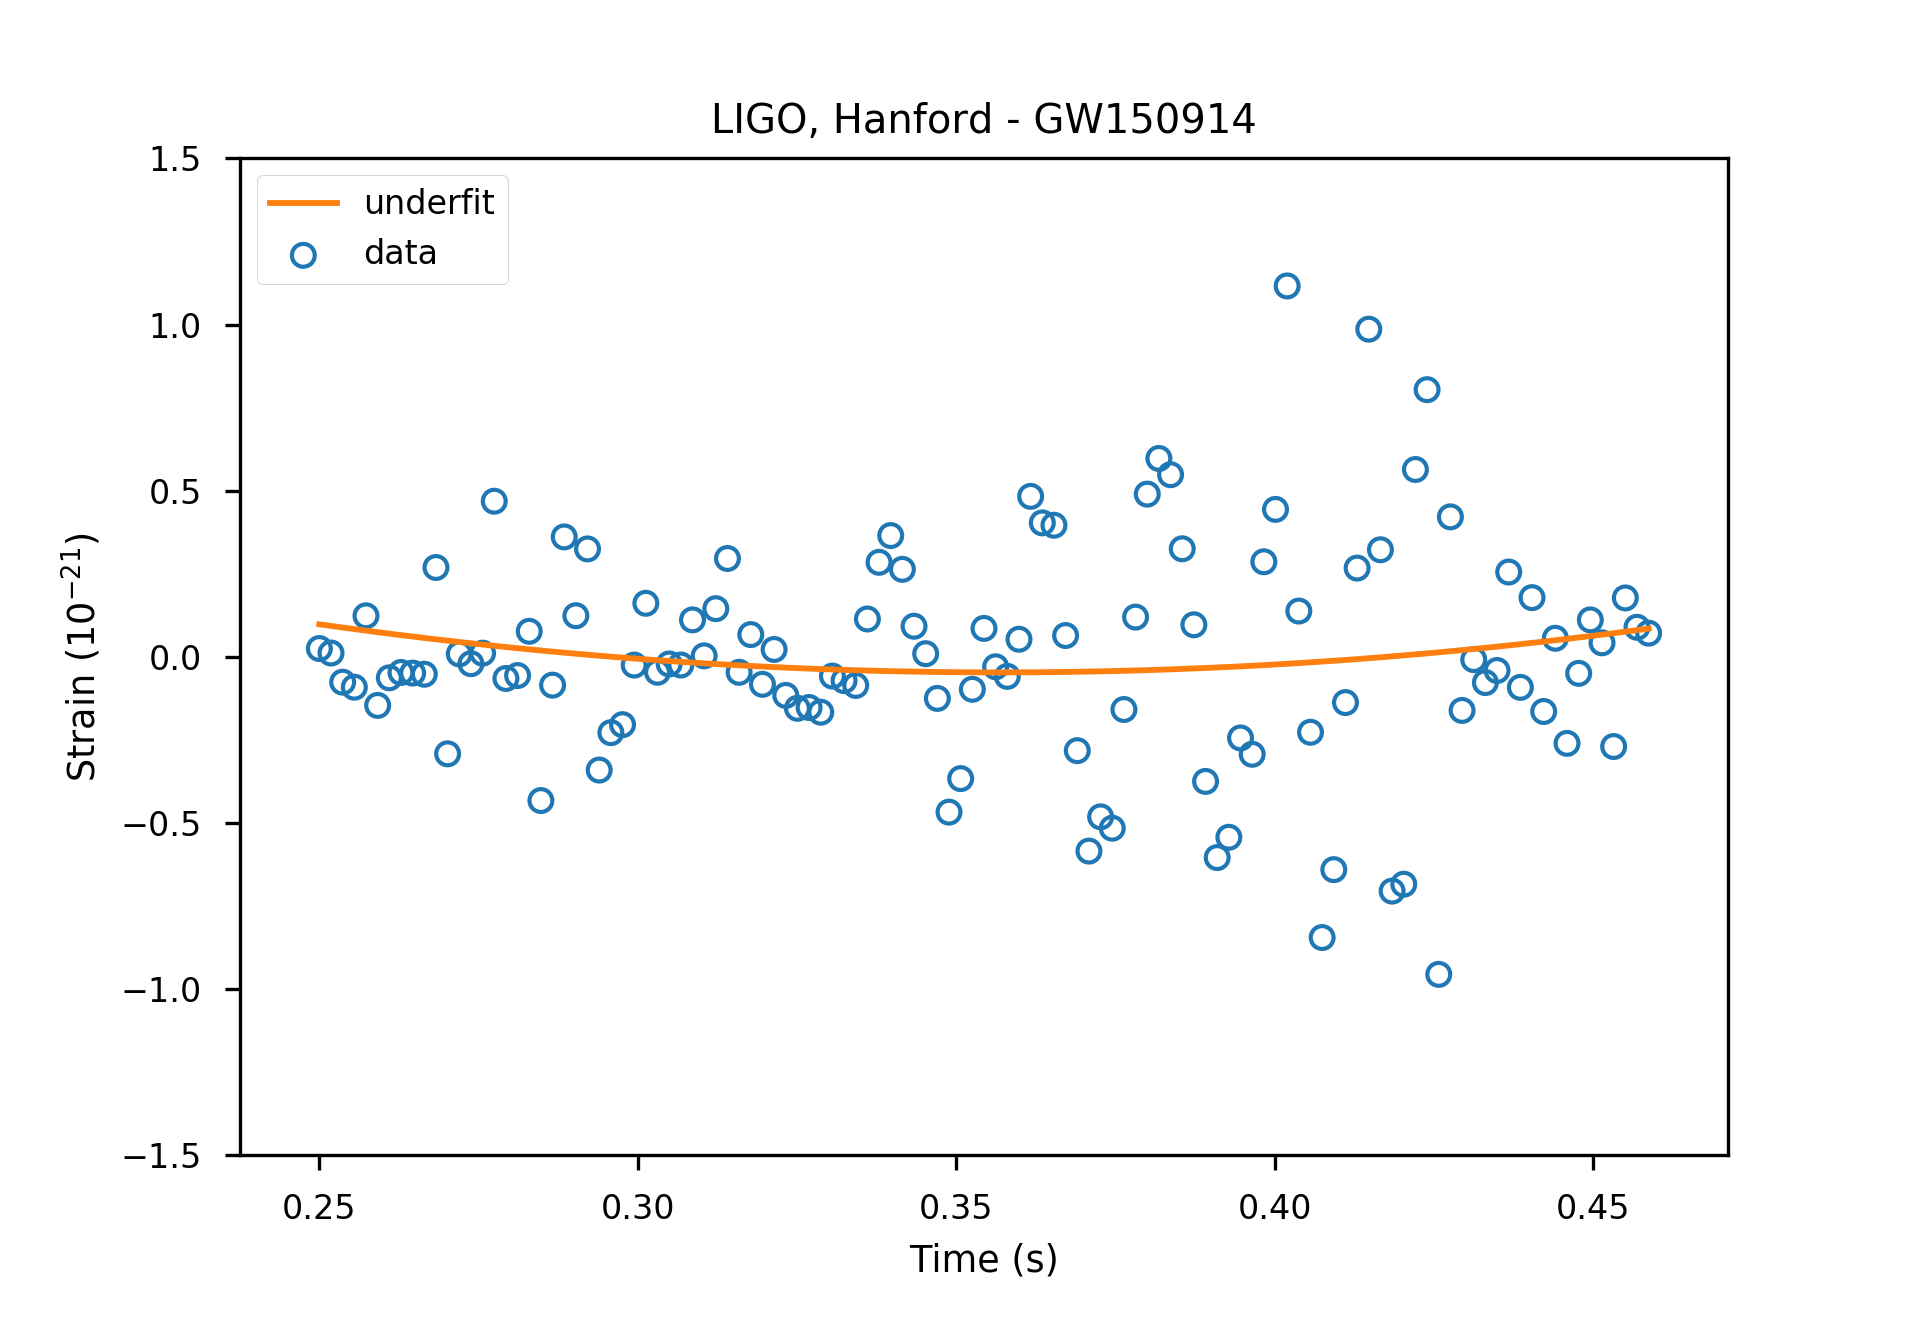
\includegraphics[width=0.5\textwidth]{part1/regression_underfit.png}
	  		\label{fig:regression}%
	  	}%
	  	%\hfill%
	  	\subfloat[]{%
	  		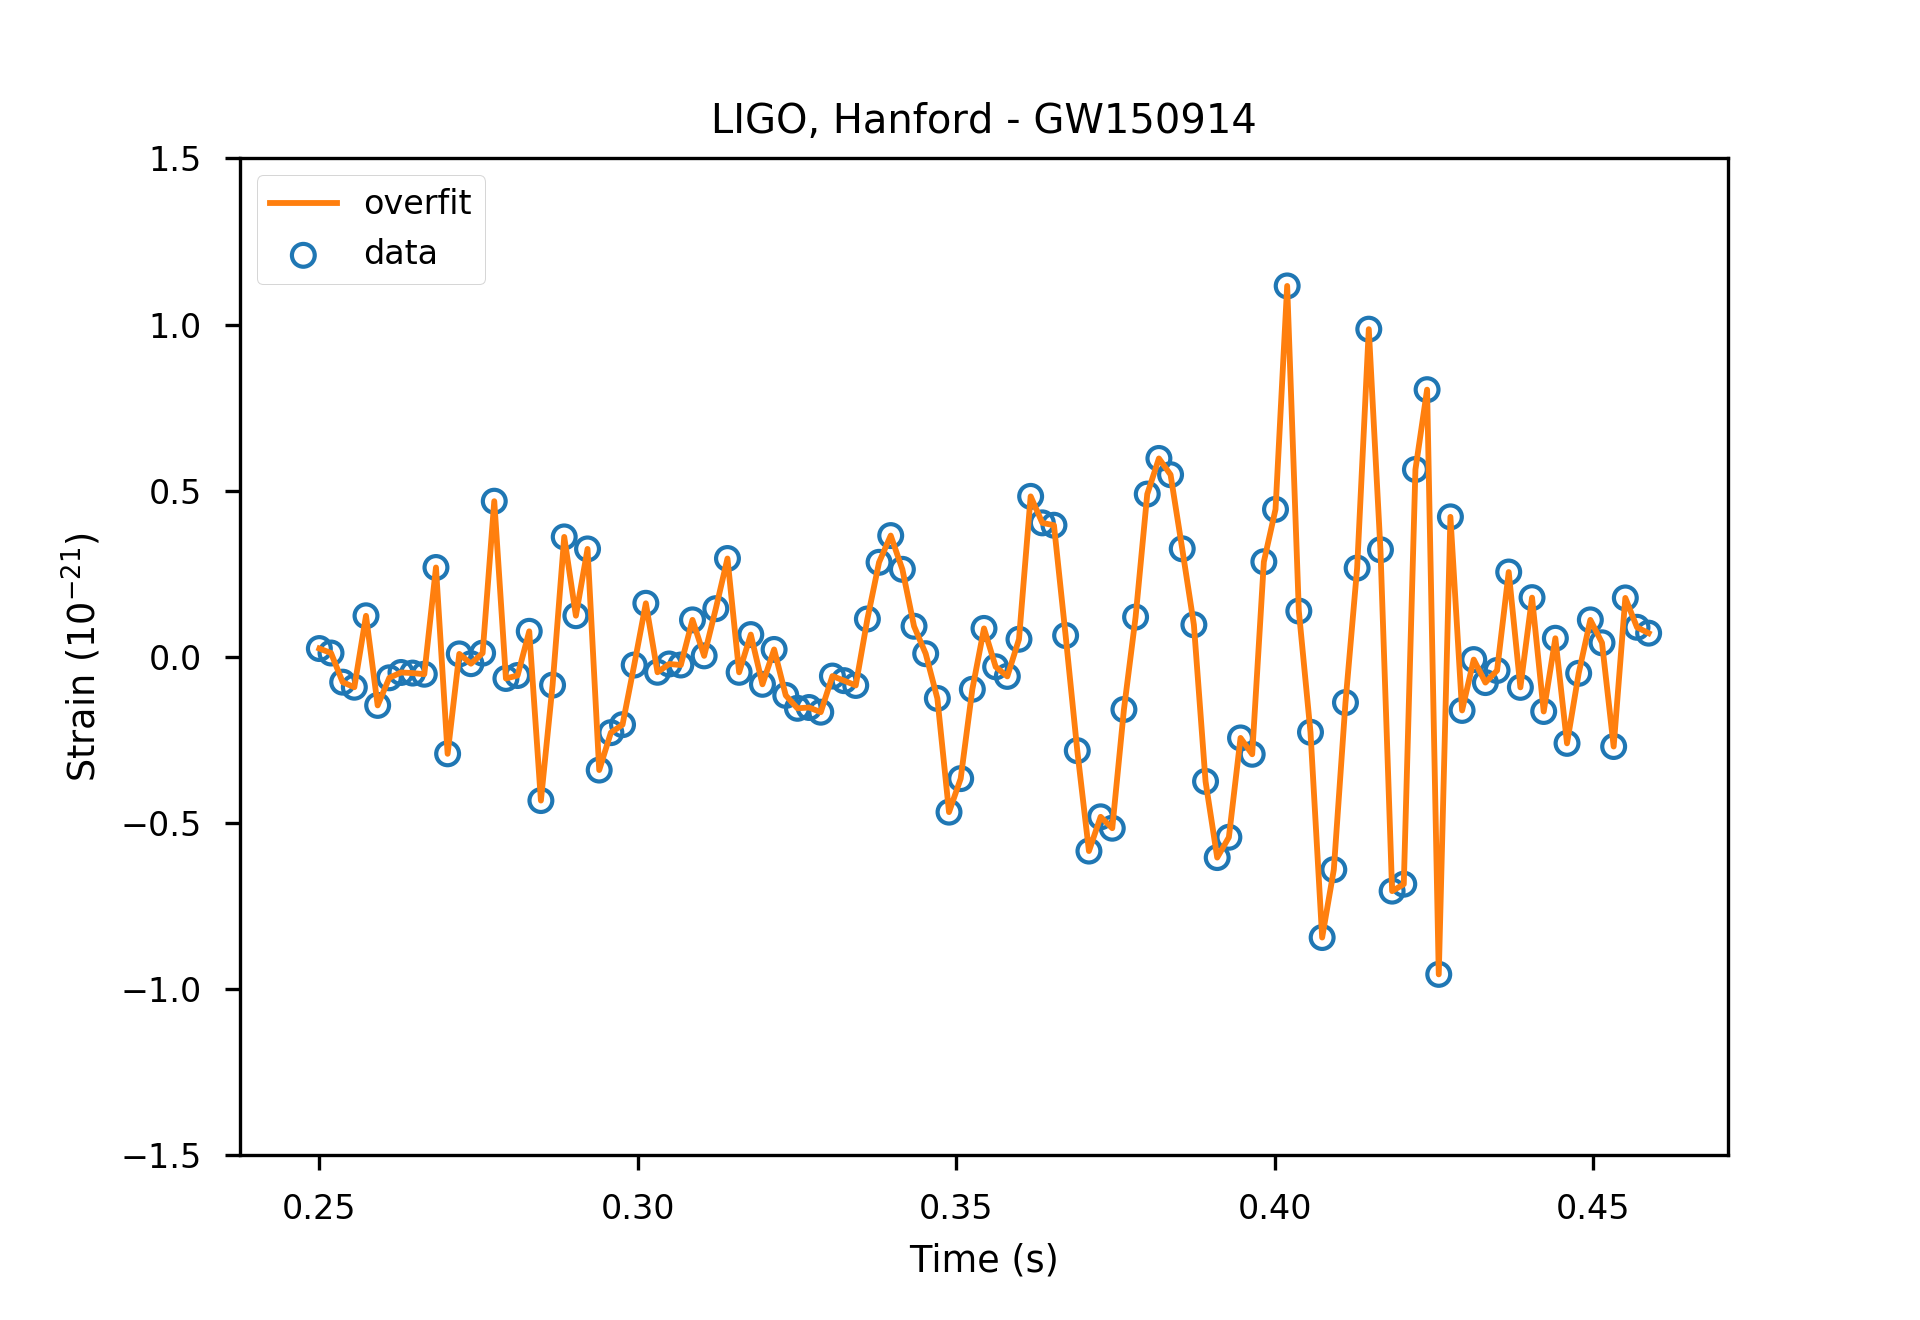
\includegraphics[width=0.5\textwidth]{part1/regression_overfit.png}
	  		\label{fig:regression}%
	  	}%
	      \hfill%
	  	\subfloat[]{%
	  		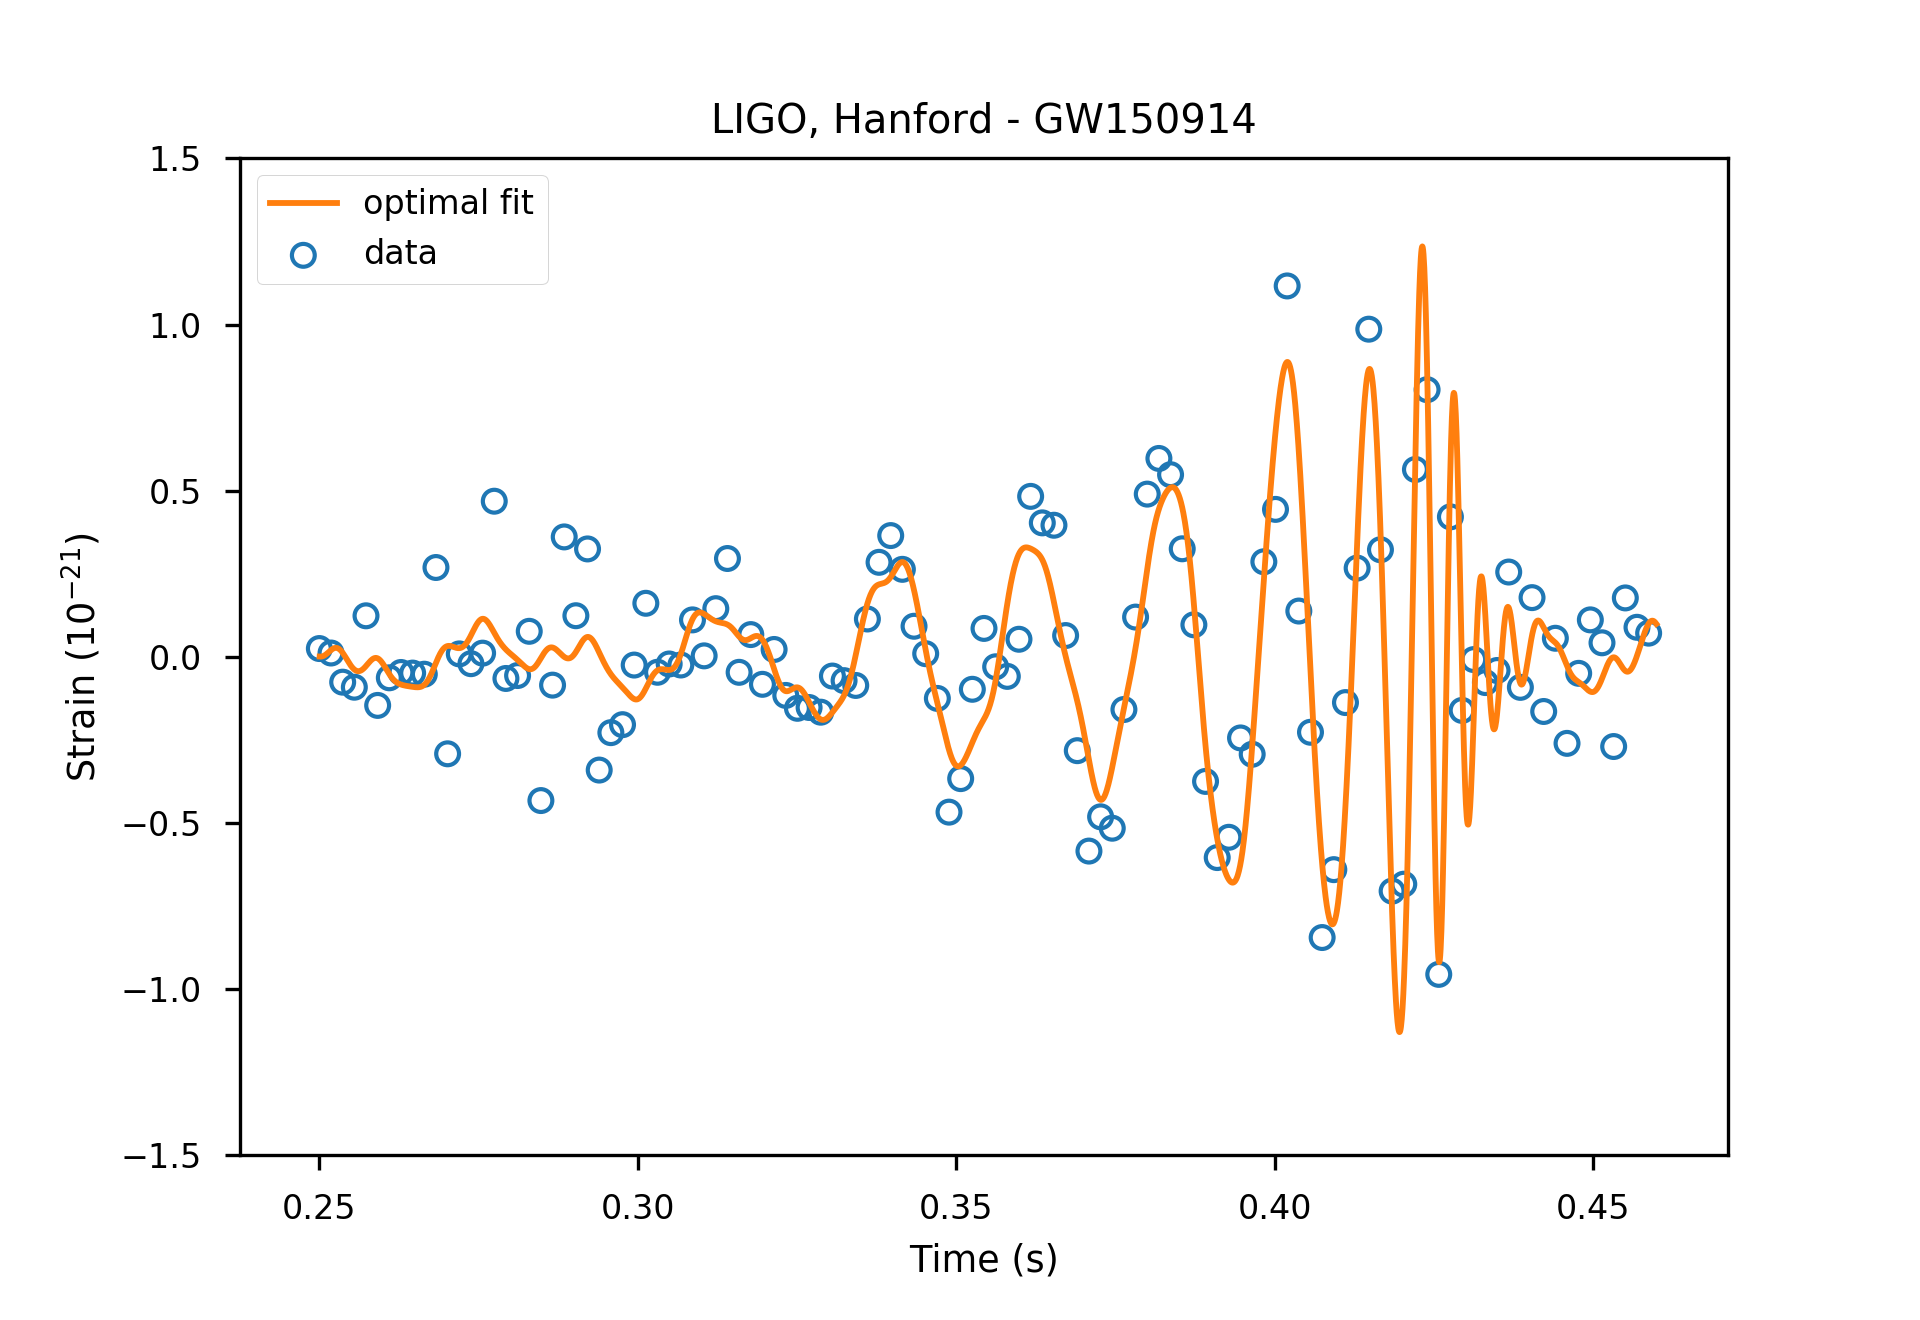
\includegraphics[width=0.5\textwidth]{part1/regression_fit.png}
	  		\label{fig:regression}%
	  	}%
	  	\caption{An example of underfit (a), overfit (b) and optimal fit (c) for a nonlinear regression problem. The data are a downsampled version ($f_s = 546~Hz$) of the first observation of gravitational waves from a binary black hole merger detected on September 14\textsuperscript{th}, 2015, 09:50:45 {\sc utc} at LIGO Hanford (WA).}\label{fig:regression_fit}
	  \end{figure}

	  \begin{figure}[!h]
			\centering
			\subfloat[]{%
				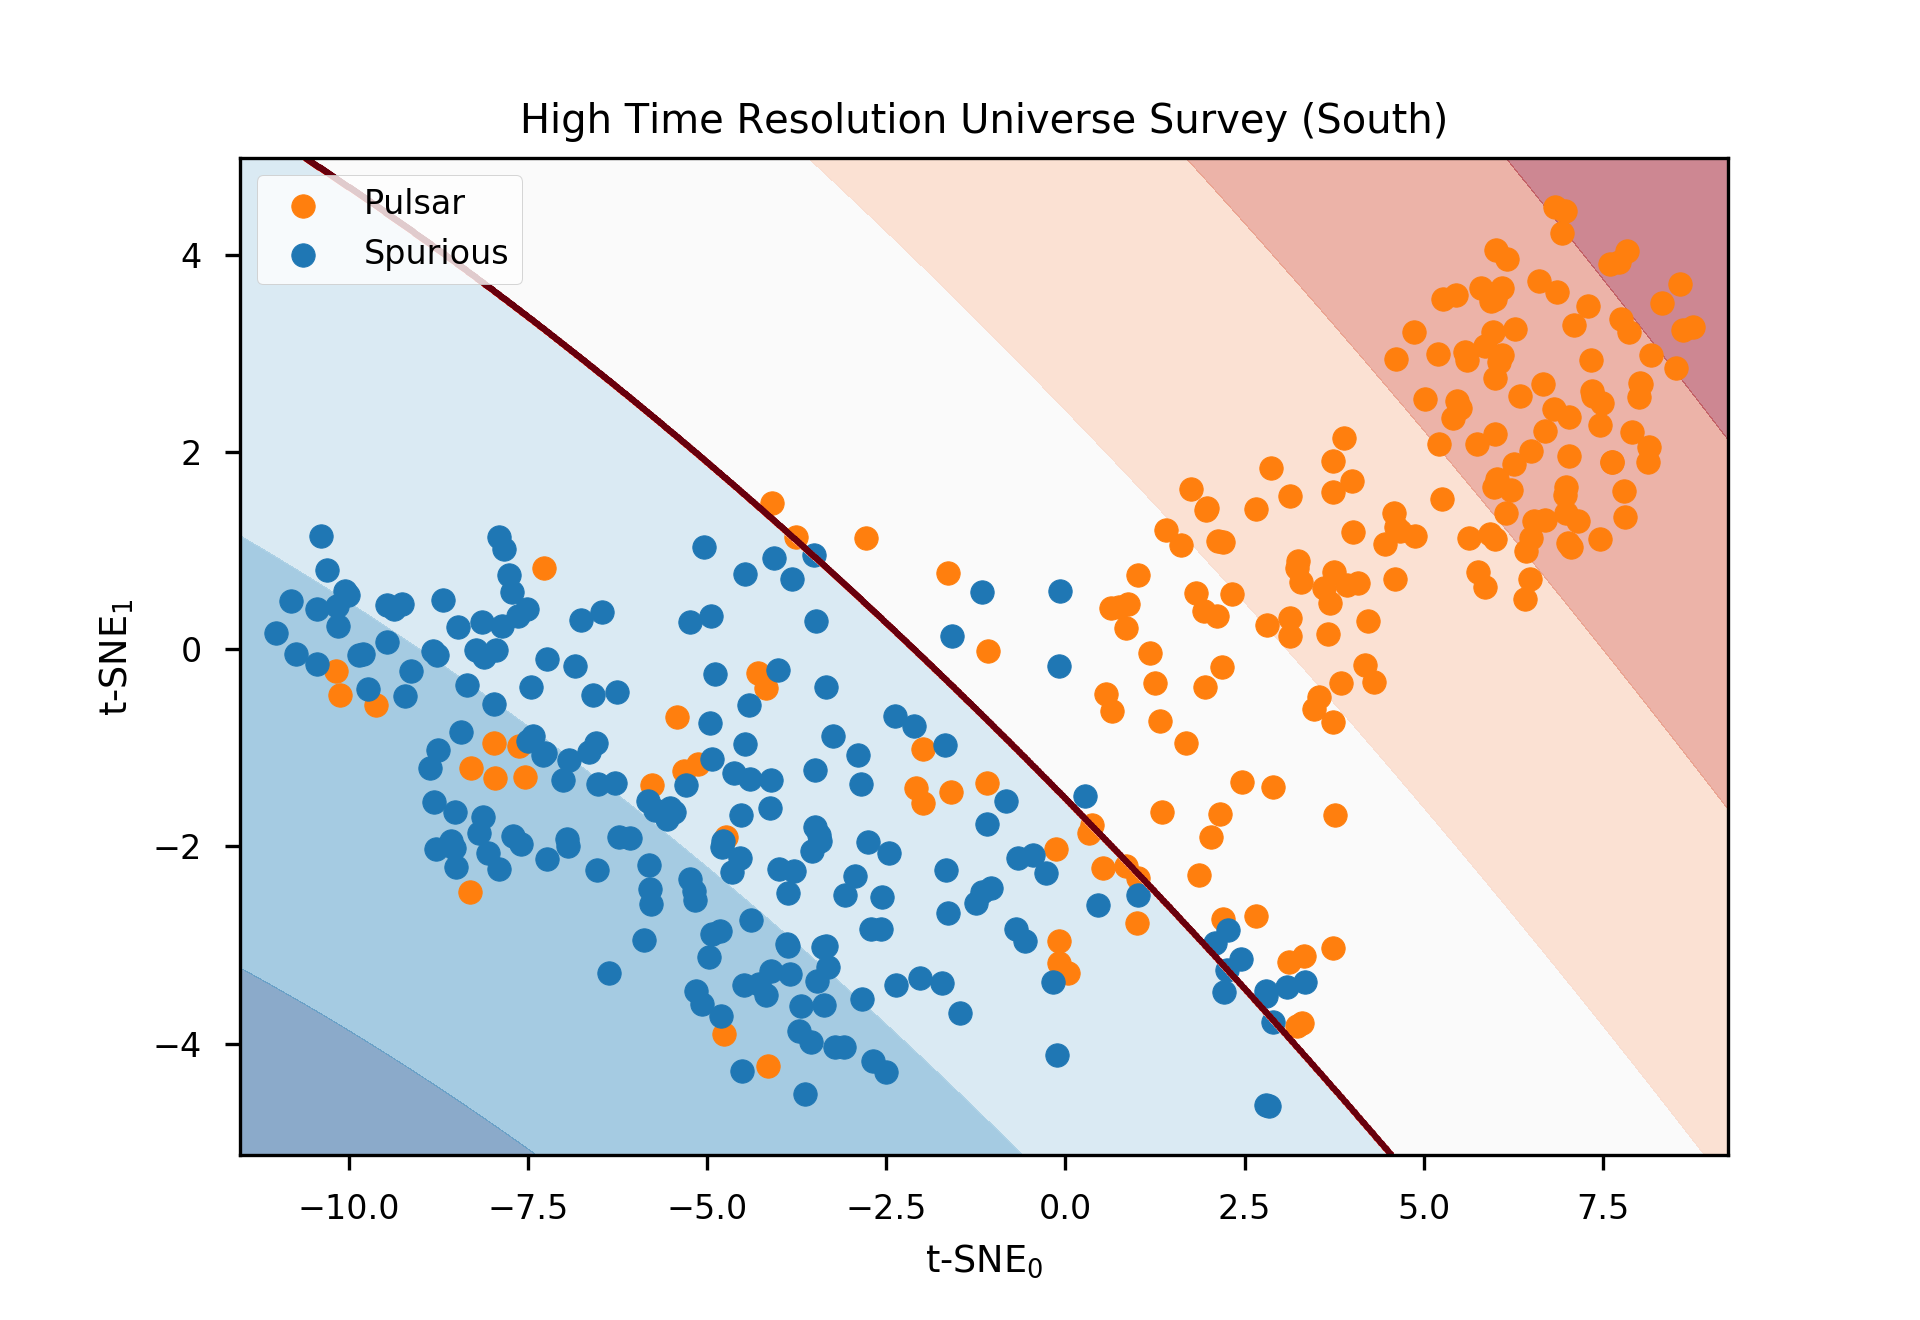
\includegraphics[width=0.5\textwidth]{part1/classification_underfit.png}
				\label{fig:regression}%
			}%
			%\hfill%
			\subfloat[]{%
				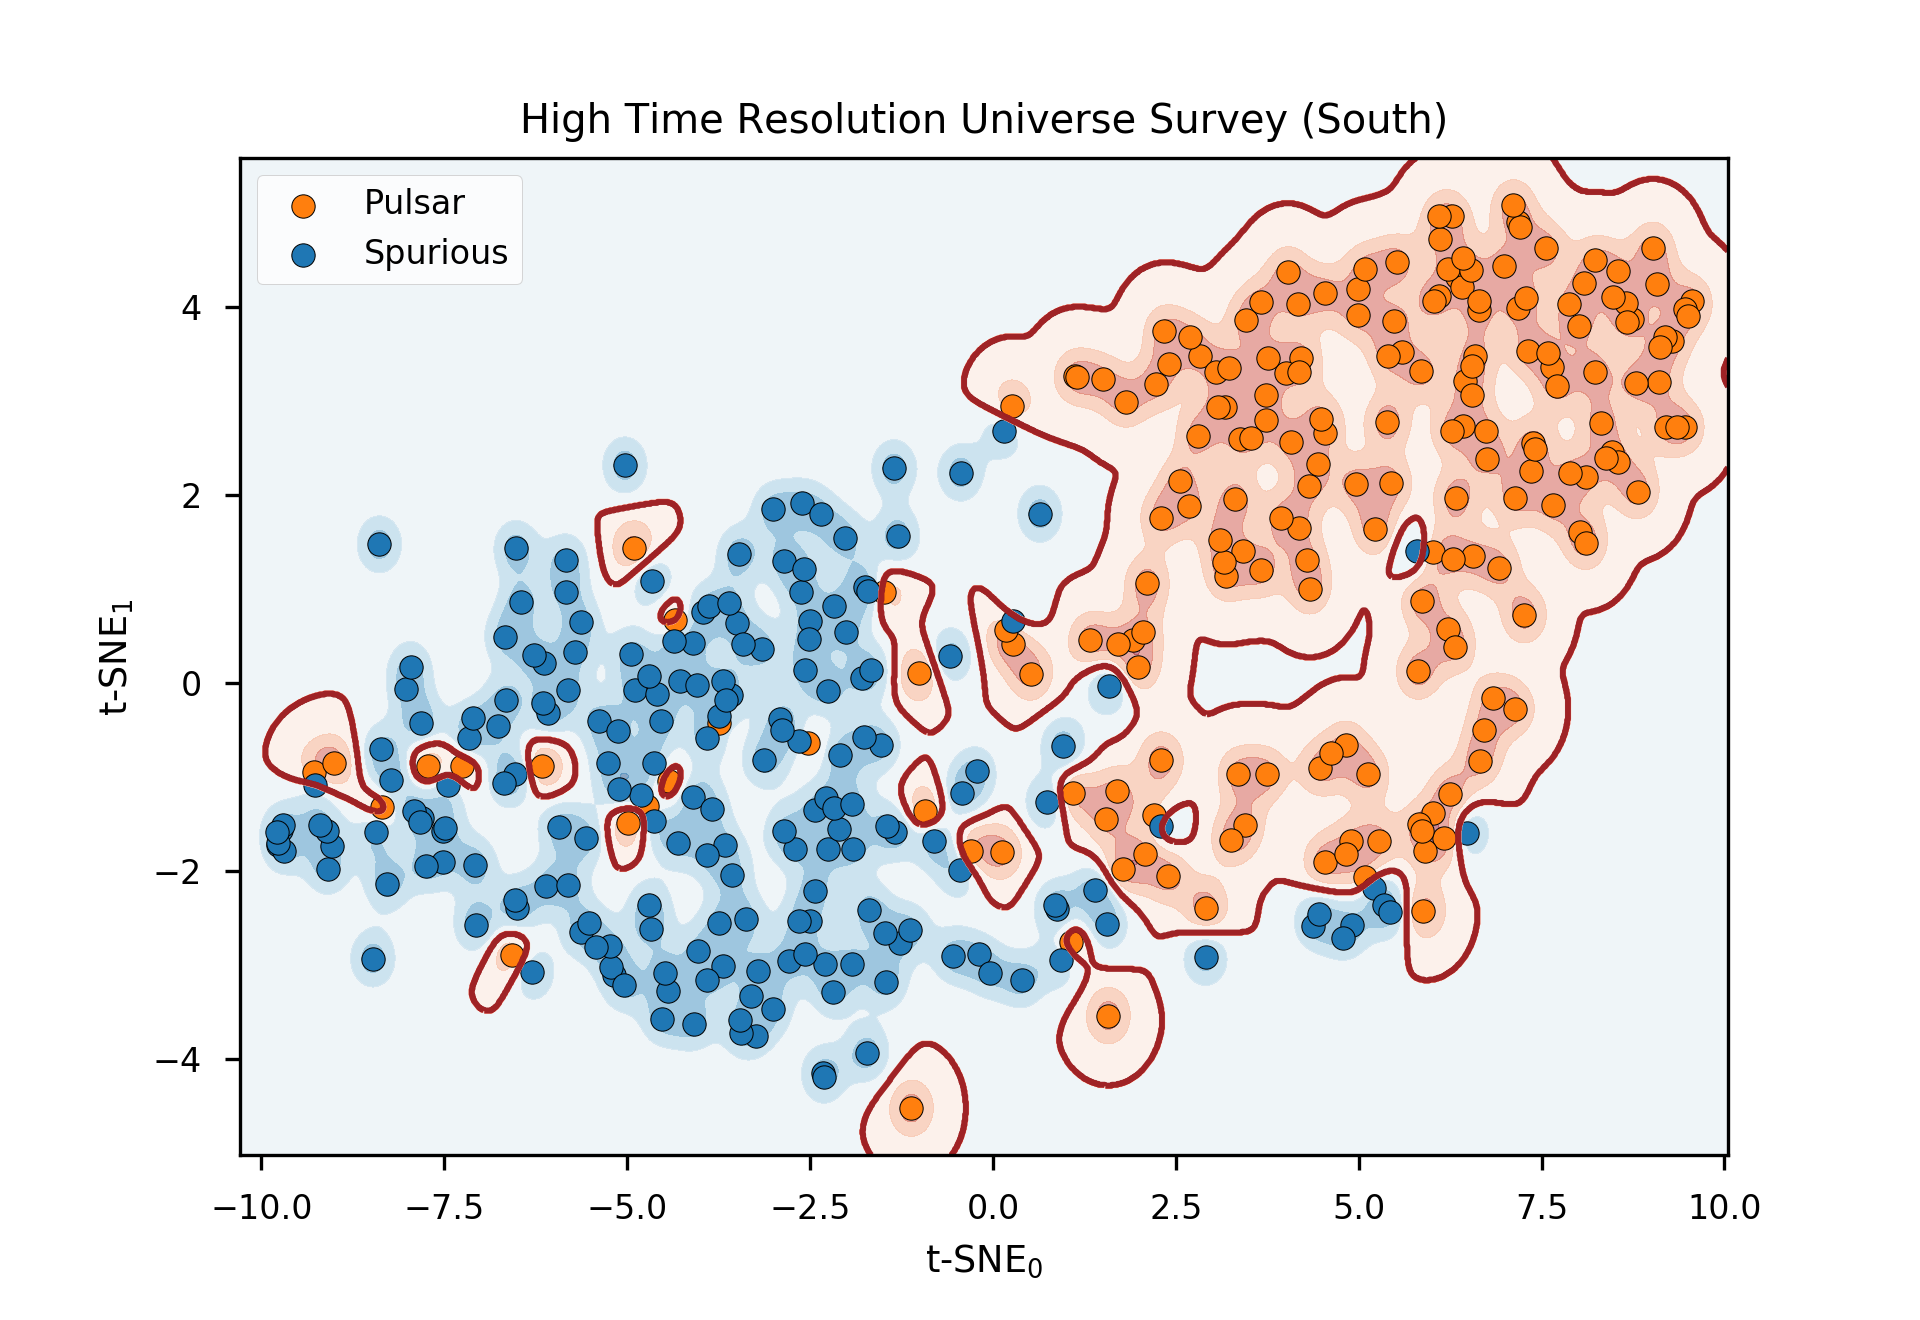
\includegraphics[width=0.5\textwidth]{part1/classification_overfit.png}
				\label{fig:regression}%
			}%
			\hfill%
			\subfloat[]{%
				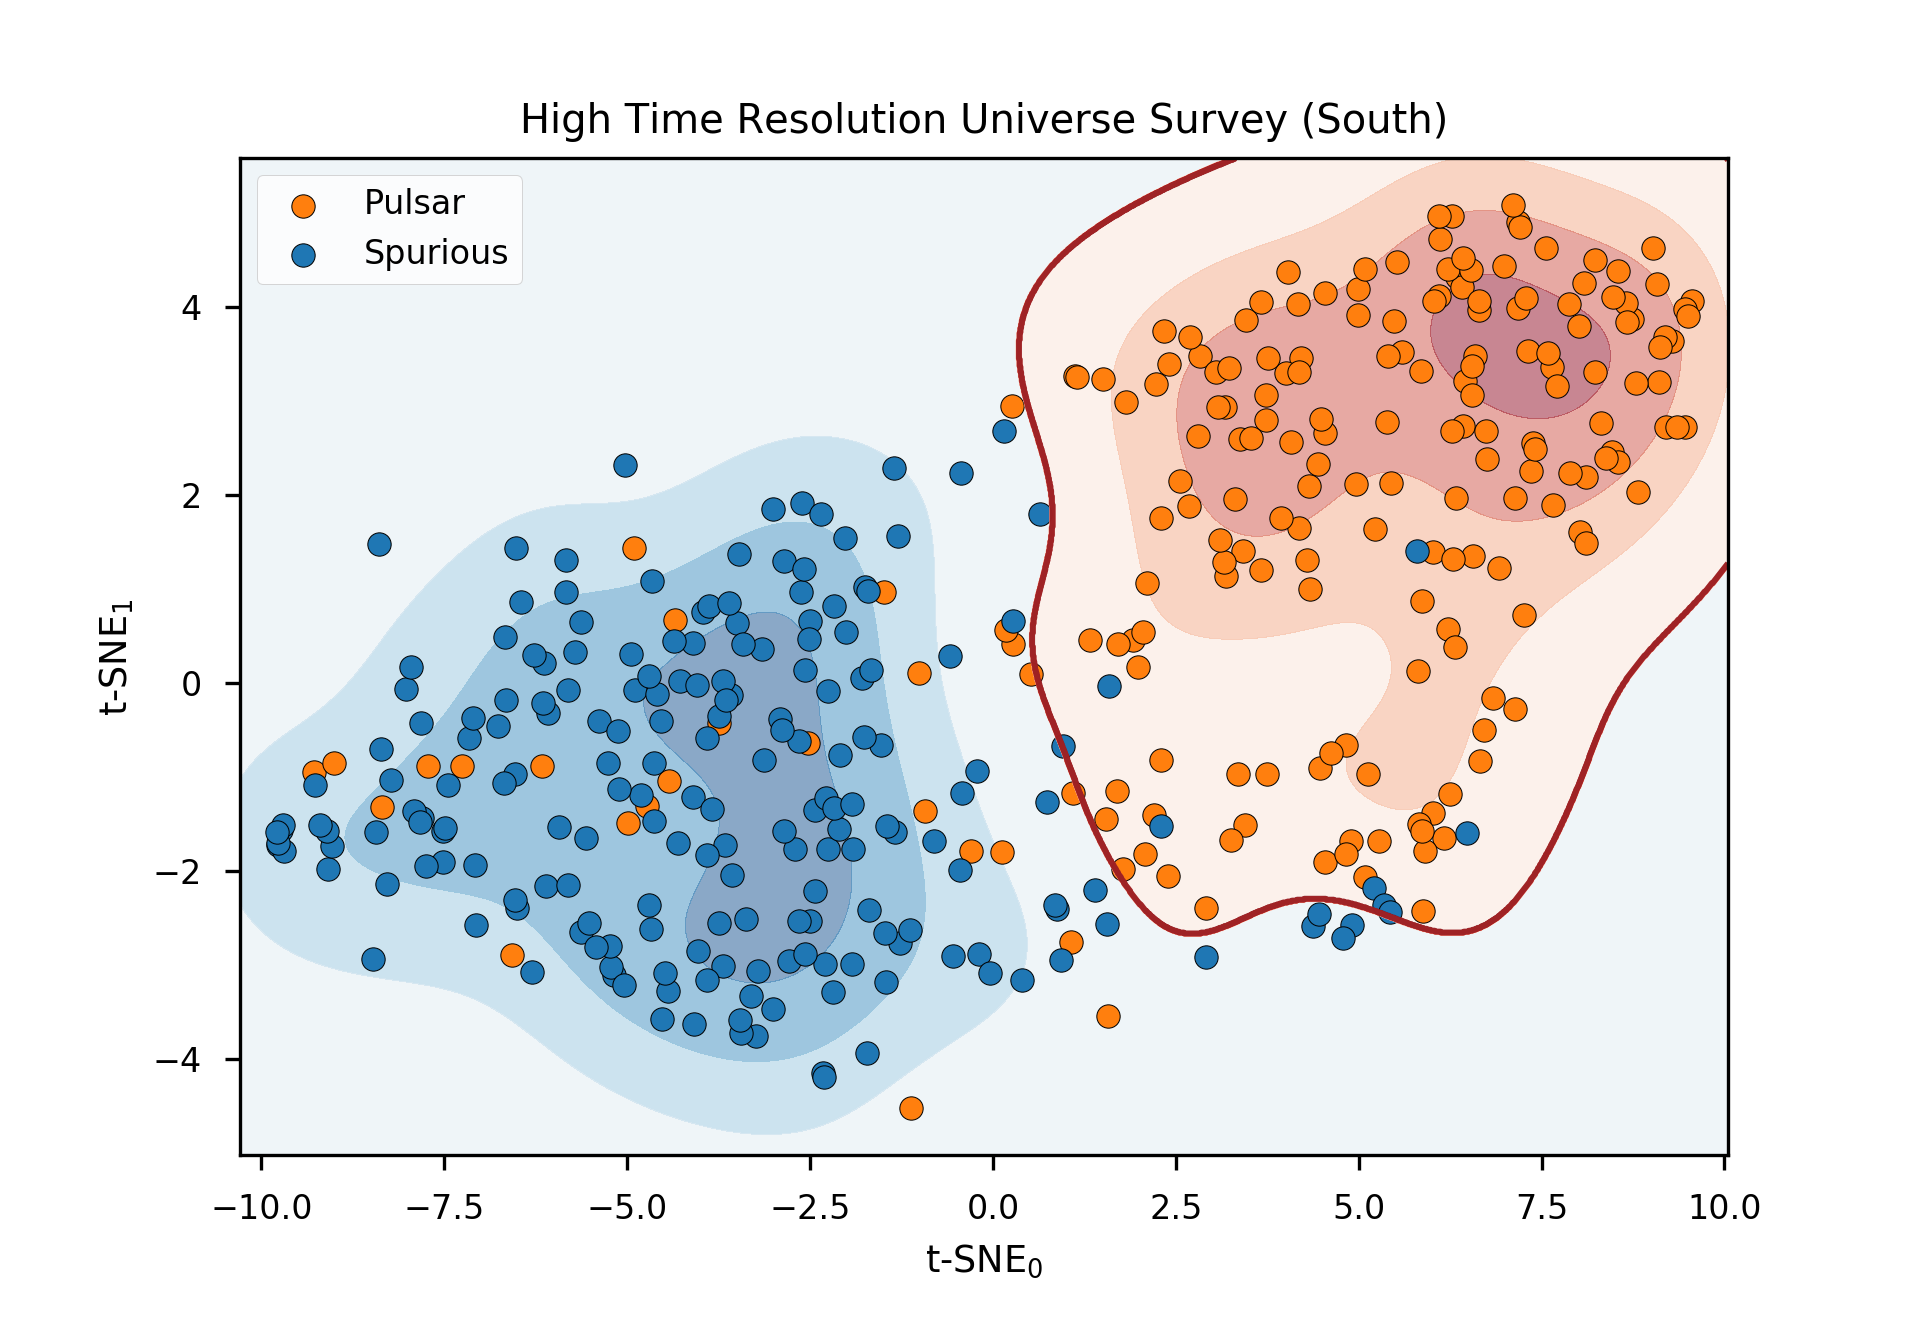
\includegraphics[width=0.5\textwidth]{part1/classification_fit.png}
				\label{fig:regression}%
			}%
			\caption{An example of underfit (a), overfit (b) and optimal fit (c) for a nonlinear binary classification problem. Each data point is a pulsar candidate randomly sampled from the High Time Resolution Universe Survey (South) dataset. The data are standardized and their dimensionality is reduced by the \ac{t-SNE} algorithm~\cite{van2008visualizing}. }\label{fig:classification_fit}
	  \end{figure}


%	    Real-world data collections can be heavily affected by random noise,
%	    As the biomedical world is the the main area of interest of this thesis (see Section~\ref{sec:challenges_biomedical}),
%	    The most widely adopted common strategy to build predictive models out of noisy data is called \textit{regularization}.
      In ML literature, \textit{regularization} is the most important countermeasure to overfitting and it is widely adopted, under several forms, to build predictive models out of noisy data.

	    The original contribution of this PhD thesis mainly relies on the application of data science and ML concepts to noisy domains. Therefore, regularization strategies are of primary interest in this discussion.
	    For each learning algorithm described, particular emphasis will be put on the relevant regularization strategies.

	    In its broader definition \textit{regularization} can be seen as the process of introducing additional information in order to solve a possibly ill-posed problem.
			As shown in Equation~\eqref{eq:losspen}, this is typically translated in the use of a regularization penalty $\mathcal{R}(f)$, controlled by a regularization parameter $\lambda$ \cite{tikhonov1963solution, evgeniou2000regularization}.

	     \begin{equation}\label{eq:losspen}
	    	\argmin_{f \in \mathcal{F}} \frac{1}{n}\sum_{i=1}^n L(f(\bm{x}_i),y_i) + \lambda \mathcal{R}(f)
	    \end{equation}

			% The expected result is a function that fits the training data while having good generalization properties, \ie accurate predictions on previously  \textit{unseen} test data \cite{hastie2009elements}.
			Choosing different $\mathcal{R}(f)$ implies inducing different effects on the solution and it also leads to the definition of different learning machines (see Section~\ref{subsec:regularization_methods}).
			With the regularization parameter $\lambda$ it is possible to control the trade-off between adherence to the training data and strength of the effect induced by $\mathcal{R}(f)$.
			As an example, we can think of using a penalty that induces smoothness, such as the $\ell_2$-norm, or sparsity, such as the $\ell_1$-norm, in the solution.
			A pictorial representation of a learning machine working in overfitting, underfitting and optimal fitting regime in a regression and a classification case can be seen in
			Figure~\ref{fig:regression_fit}~\footnote{source \url{https://losc.ligo.org/events/GW150914/}}
			and
		  Figure~\ref{fig:classification_fit}~\footnote{source \url{https://archive.ics.uci.edu/ml/datasets/HTRU2}}, respectively.


	%    The regularization penalty $R(f)$ imposes stability on the expected function exploiting the available prior knowledge on the problem~\cite{tikhonov1963solution}. More details on $R(f)$ will be given in the next section.

	    Supervised learning machines may rely on very different mathematical backgrounds such as generalized linear models, nonlinear deep neural networks, kernels, trees, ensemble of trees, \etc. Nevertheless, disregarding their nature, they all share the common structure defined in Equation~\eqref{eq:losspen}.
	    The solution of this problem can be achieved either by Empirical (or Structured) Risk Minimization (\ac{ERM}) either by Maximum Likelihood/A Posteriori (\ac{MLE}/\ac{MAP}) Estimation. See Appendix~\ref{appendix:A} for more details on this two strategies, and their connection.

	    \subsection{Regularization methods} \label{subsec:regularization_methods}
	    Regularization methods is a broad class of models that include linear and nonlinear techniques for both regression and classification. The main characteristic of the methods falling in this class, is that they are particularly straightforward to express as in Equation~\eqref{eq:losspen}. In fact, as described in~\cite{evgeniou2000regularization}, they are easily identifiable by the use of one loss function $L(f(\bm{x}), y)$ and one, or more, regularization penalty $\mathcal{R}(f)$.

	    In the following sections an overview of the most popular regularization methods is presented.

			%%%%%%%%%%%%%%%%%%%%%%%%%%%%%%%%%%%%%%%
			\subsubsection{Ordinary least squares} \label{sec:ols}
			We start this discussion focusing on linear models $\hat y = f(\bm{x})=\bm{x}^T\bm{w}$ and taking into account the most popular loss function for regression problems: the square loss $L(\hat y, y) = (\bm{x}^T\bm{w}-y)^2$. The data fitting problem expressed in Equation~\eqref{eq:ols} is known as \textit{Ordinary Least Squares} (\ac{OLS}), or simply as \textit{linear regression}, and it does not include any regularization term.

			\begin{equation} \label{eq:ols}
				\bm{\hat w}_{\text{OLS}} = \argmin_{\bm{w} \in \mathbb{R}^d} \frac{1}{n} \sum_{i=1}^n (\bm{x}_i^T\bm{w} - y_i)^2 = \argmin_{\bm{w} \in \mathbb{R}^d} \frac{1}{n} \norm{X\bm{w} - \bm{y}}_2^2
			\end{equation}

			The minimization problem in Equation~\eqref{eq:ols} is convex and differentiable, hence its solution can be achieved in closed-form as
			$$
				\bm{\hat w}_{\text{OLS}} = (X^TX)^{-1}X^T\bm{y}
			$$
			or by iterative minimization routines such as (stochastic) gradient descent-like algorithms~\cite{boyd2004convex, sra2012optimization}. A pictorial representation of the solution of OLS can be seen in Figure~\ref{fig:w_ols}.

			In case of multiple regression tasks, the OLS approach can be extended to vector-valued regression as well. In this case the least squares problem can be written as
			\begin{equation} \label{eq:vvr_ols}
				\begin{aligned}
				\hat W_{\text{OLS}}={} & \argmin_{W \in \mathbb{R}^{d \times k}} \frac{1}{n} \sum_{i=1}^n \sum_{t=1}^k (\bm{x}_i^T\bm{w}^t - y_i^t)^2  \\
				& =	\argmin_{W \in \mathbb{R}^{d \times k}} \frac{1}{n} \norm{XW - Y}_F^2
				\end{aligned}
			\end{equation}
			where $\norm{A}_F= \sqrt{\sum_{i=1}^n\sum_{t=1}^k |a_i^t|^2}$ is the \textit{Frobenius} norm (also known as  \textit{Hilbert-Schmidt} norm) and it can be considered as an extension of the $\ell_2$-norm to the matrix case.
			Lacking of appropriate regularization penalties, solving the problem in Equation~\eqref{eq:vvr_ols} corresponds to solving $k$ isolated regression problems, one for each task.
			The vector-valued OLS approach, even if theoretically legit, is rather uncommon in practical applications and a regularized version of Equation~\eqref{eq:vvr_ols} is typically preferred (see following sections).

			Even though mainly used for regression, the square loss can also be used to solve binary classification problems (see Table~\ref{tab:losses}). In this case, it can be rewritten as
			\begin{equation} \label{eq:margin_square_loss}
				(\bm{x}^T\bm{w}-y)^2 = (1-y \cdot \bm{x}^T\bm{w})^2
			\end{equation}
			exploiting the fact that the two classes are encoded with binary labels: $\bm{y} \in \{+1,-1\}^n$. For multiclass classification problems, strategies such as \textit{One-vs-One} (\ac{OVO}) or \textit{One-vs-All} (\ac{OVA}) can be adopted to reduce the problem to multiple binary classifications~\cite{hastie2009elements}.

			OLS is probably the most na\"ive prediction strategy, nevertheless it is widely adopted in several studies. Let's see what happens when we use the OLS model on a real regression problem.

			For this example, and the following ones, we take into account the dataset $\mathcal{D}_{\text{aging}} = \{(\bm{x}_i, y_i)\}_{i=1}^{n=111}$ where each input sample $\bm{x}_i \in \mathbb{R}^{12}$ presents a set of measures describing the metabolic state of a healthy subject and $y_i \in \mathbb{N}_+$ is its age expressed in years.
			For the sake of this discussion a  thorough description of $\mathcal{D}_{\text{aging}}$ at this point is irrelevant\footnote{this regression problem is widely described and analyzed in Chapter~\ref{chap:frassoni}.}, we can simply think as the $d=12$ variables as predictors of the outcome $y$ and we look for some linear input-output relationship.
			In order to do that, we randomly split $\mathcal{D}_{\text{aging}}$ in two chunks obtaining a training and a test set of $n_{\text{tr}}=74$ and $n_{\text{ts}}=37$ samples respectively. Then, we fit the OLS model on the training set obtaining the weights vector $\bm{\hat w}_{\text{OLS}}$ represented in Figure~\ref{fig:coefs_ols}.
			\begin{figure}[!h]
				\centering
				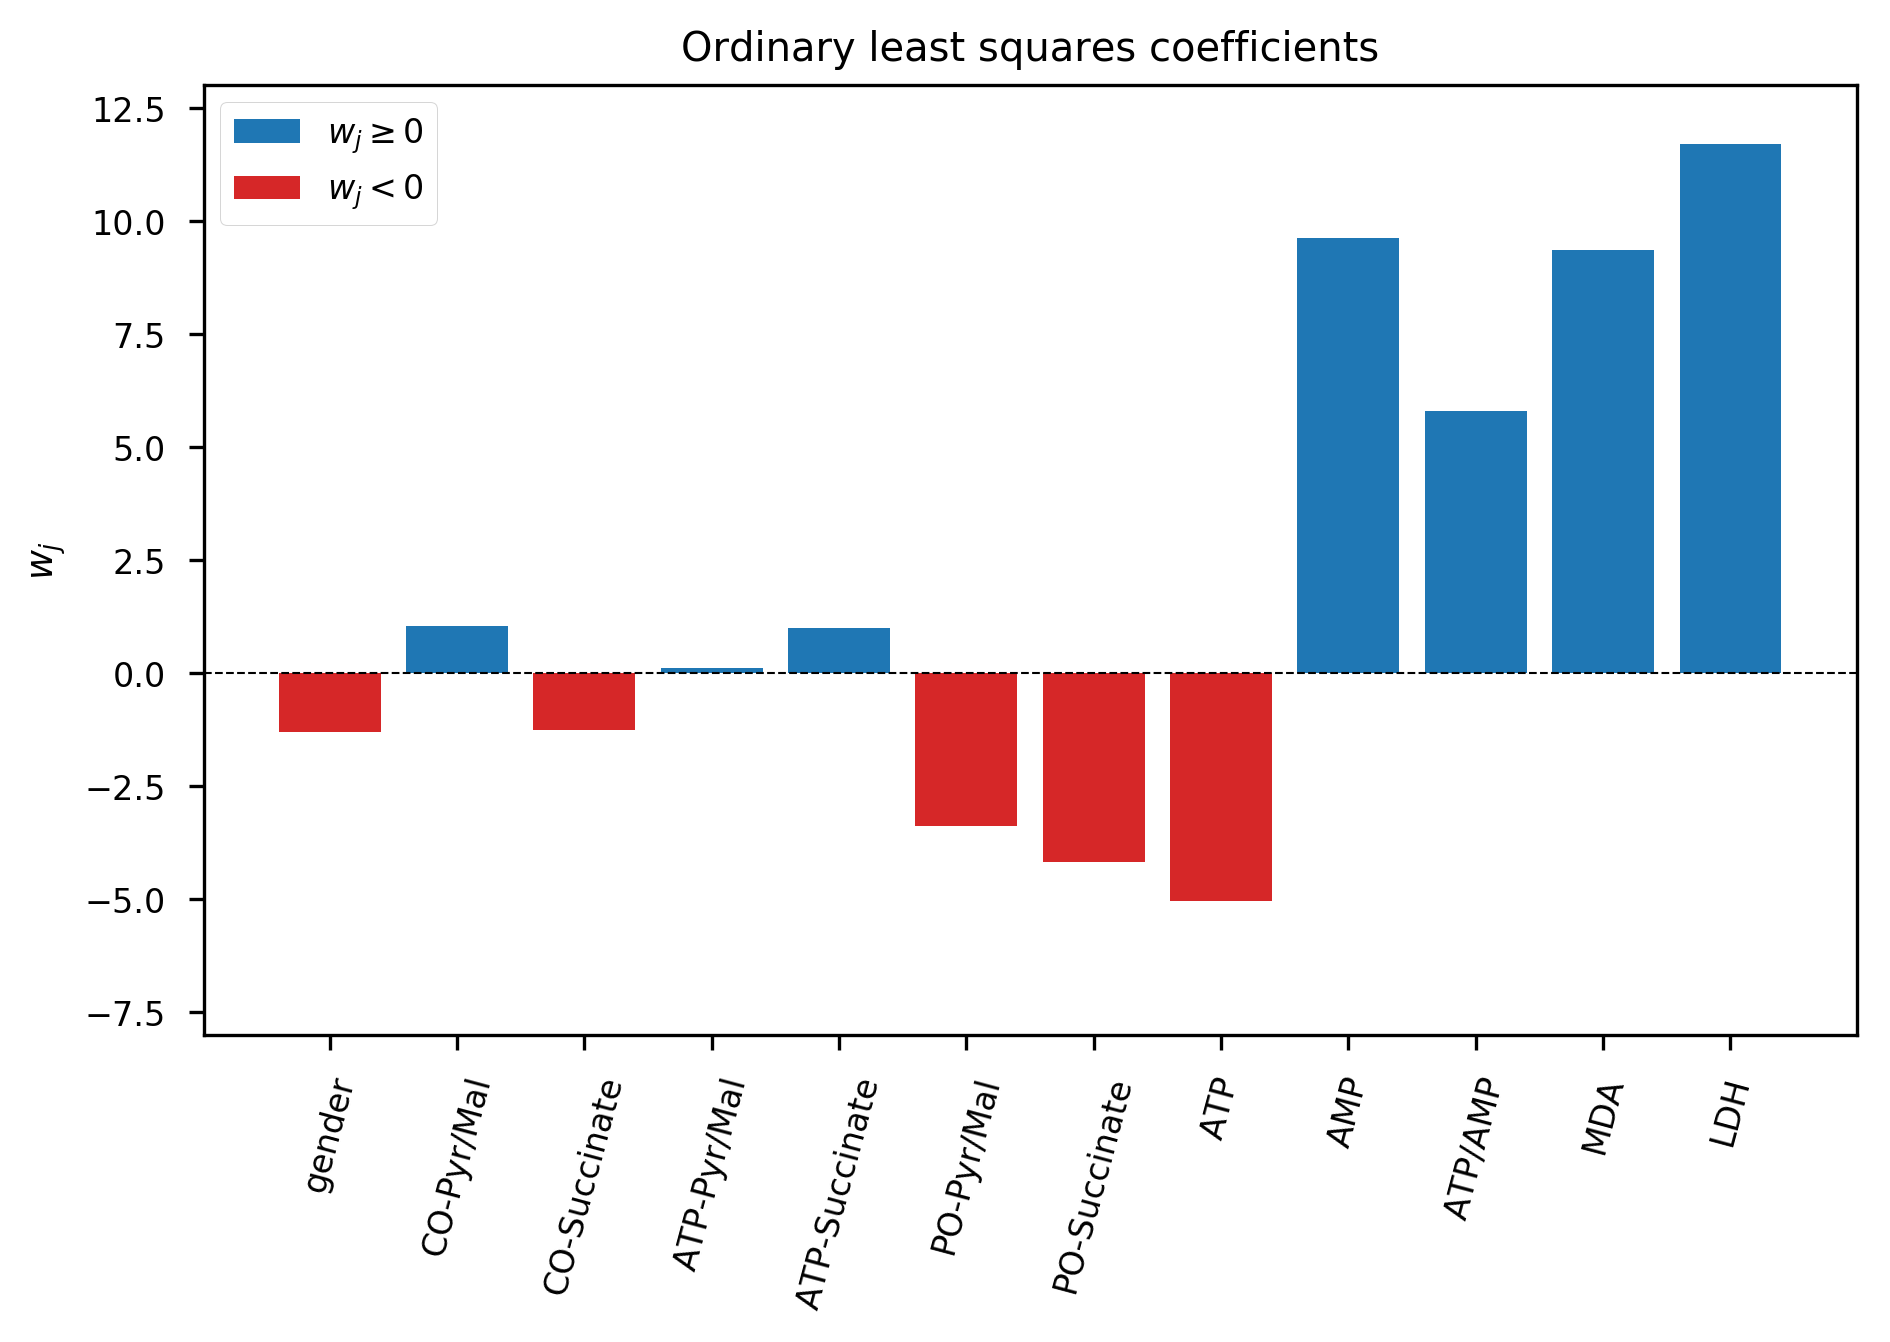
\includegraphics[width=0.8\textwidth]{part1/coefs_ols.png}
				\caption{A pictorial representation of the vector $\bm{\hat w}_{\text{OLS}}$ obtained fitting an OLS model on $74$ randomly selected training samples of $\mathcal{D}_{\text{aging}}$. Variables associated with positive (\ie directly proportional to the output) and a negative (\ie inversely proportional) weight are represented in blue and red, respectively.} \label{fig:coefs_ols}
		  \end{figure}
			As we can see, in order to achieve a predictive model, OLS can only spread the weights across all the input variables. Evaluating $\bm{\hat w}_{\text{OLS}}$ on the test set, this model has a Mean Absolute Error (\ac{MAE}) of $10.598$ years and explains the $74.29\%$ of the variance.

			This result looks promising, but we will see in the next sections whether they can be improved with the use of some regularization penalty.

%			We have already pointed out that learning predictive functions only by minimizing a loss function may lead to suboptimal solutions; therefore in the following sections we will explore pro and cons of using different penalties.

			\subsubsection{Ridge regression} \label{sec:ridge_regression}
			In its original proposition, \textit{ridge regression}~\cite{hoerl1970ridge} is defined as a least squares problem penalized by the squared $\ell_2$-norm of the regression coefficients, see Equation~\eqref{eq:l2}.

			\begin{equation}\label{eq:l2}
				\mathcal{R}_{\mbox{$\ell_2$}}(\bm{w}) = \sum_{j=1}^d (w_j)^2 = \norm{\bm{w}}_2^2
			\end{equation}

			Therefore, the ridge regression minimization problem can be written as in Equation~\eqref{eq:ridge_regression}.

			\begin{equation} \label{eq:ridge_regression}
				\bm{\hat w}_{\ell_2} = \argmin_{\bm{w} \in \mathbb{R}^d} \frac{1}{n} \sum_{i=1}^n (\bm{x}_i^T\bm{w} - y_i)^2 + \lambda  \sum_{j=1}^d (w_j)^2 = \argmin_{\bm{w} \in \mathbb{R}^d} \frac{1}{n} \norm{X\bm{w} - \bm{y}}_2^2 + \lambda \norm{\bm{w}}_2^2
			\end{equation}

			This penalty leads to smooth solutions as it shrinks the coefficients toward zero, but it does not achieve a parsimonious representation, as it always keep all the variables in the model.
			The ridge regression problem of Equation~\eqref{eq:ridge_regression} is convex  and differentiable and a pictorial representation of its solution in a 2D case is depicted in Figure~\ref{fig:w_ridge}. The ridge coefficients $\bm{\hat w}_{\ell_2}$ can be estimated in closed-form as
			$$
				\bm{\hat w}_{\ell_2} = (X^TX + \lambda n I)^{-1}X^T\bm{y}
			$$
			where $I$ is the $d \times d$ identity matrix. An estimate for the ridge coefficients can also be obtained with gradient descent-like optimization routines~\cite{boyd2004convex, sra2012optimization}.

			The regularization parameter $\lambda$ plays the fundamental role of balancing the trade-off between data adherence and smoothness of the solution.
			Penalizing the $\ell_2$-norm of the regression coefficients, their value is shrunk toward zero. This results in an increased robustness of the solution to the noise affecting the training data.

			In case of multiple outputs, the vector-valued ridge regression problem can be written as in Equation~\eqref{eq:vvr_ridge}.
			\begin{equation} \label{eq:vvr_ridge}
				\begin{aligned}
					\hat W_{\ell_2}={} & \argmin_{W \in \mathbb{R}^{d \times k}} \frac{1}{n} \sum_{i=1}^n \sum_{t=1}^k (\bm{x}_i^T\bm{w}^t - y_i^t)^2  + \lambda \sum_{j=1}^d \sum_{t=1}^k |w_j^t|^2\\
					& =	\argmin_{W \in \mathbb{R}^{d \times k}} \frac{1}{n} \norm{XW - Y}_F^2 + \lambda \norm{W}_F^2
				\end{aligned}
			\end{equation}
			As already seen for vector-valued OLS, the Frobenius norm penalty does not induce any task coupling, hence solving the problem in Equation~\eqref{eq:vvr_ridge} still corresponds to individually solve $k$ regression tasks.

			This method can be applied to binary classification problems by using the margin loss function of Equation~\eqref{eq:margin_square_loss}. Nevertheless, for $\ell_2$-norm penalized classification problems the use of the \textit{logistic loss} is usually preferred (see Section~\ref{sec:logistic_regression}).

			In deep learning literature, penalizing the regression coefficients with the $\ell_2$-norm is known as \textit{weight decay}~\cite{krogh1992simple}. Ridge regression can also be considered a form of  \textit{Tikhonov regularization}~\cite{tikhonov1963solution} and of \textit{regularization network}~\cite{evgeniou2000regularization}.
%			ridge regression is successfully applied in countless and heterogeneous biological studies mainly involving regression problems.
%			For instance, in~\cite{kratsch2014} the authors propose a ridge regression-based method to estimate ancestral characters from phylogenetic trees, while in~\cite{bovelstad2007} ridge regression is used to perform survival prediction from gene expression data.
			%\todo{\begin{enumerate}
			%	% \item loss: square loss
			%	% \item penalties: l2
			%	% \item use in regression, classification
			%%	\item use cases
			%%	\item extension to multi-task and multi-class
			%\end{enumerate}}
			%Ridge regression can be extended to the case of multiple-output prediction for both vector-valued regression and multi-category classification problems.
			%In the first case,

			Let's see what happens when this method is applied to a real regression problem. For ease of comparison, we take into account the dataset $\mathcal{D}_{\text{aging}}$, introduced in Section~\ref{sec:ols}.
			Compared to OLS, ridge regression has the parameter $\lambda$ that must be fixed before fitting the model. In this example, we estimated the best value $\hat \lambda_{\text{cv}}$ according to a standard grid-search cross-validation strategy~\cite{hastie2009elements}.
			This consists in fixing a range of ($30$) possible values for $\lambda$ (in a logarithmic scale from $10^{-3}$ to $10^2$) and
			pick the best value as the one achieving the lowest validation error, estimated via ($5$-fold) cross-validation.
			Therefore, once the best value for the regularization parameter is fixed ($\hat \lambda_{\text{cv}} = 20.43$), the experimental setup used for OLS is preserved.
			The ridge coefficients $\bm{\hat w}_{\ell_2}$ are represented in Figure~\ref{fig:coefs_ridge}.
			\begin{figure}[!h]
				\centering
				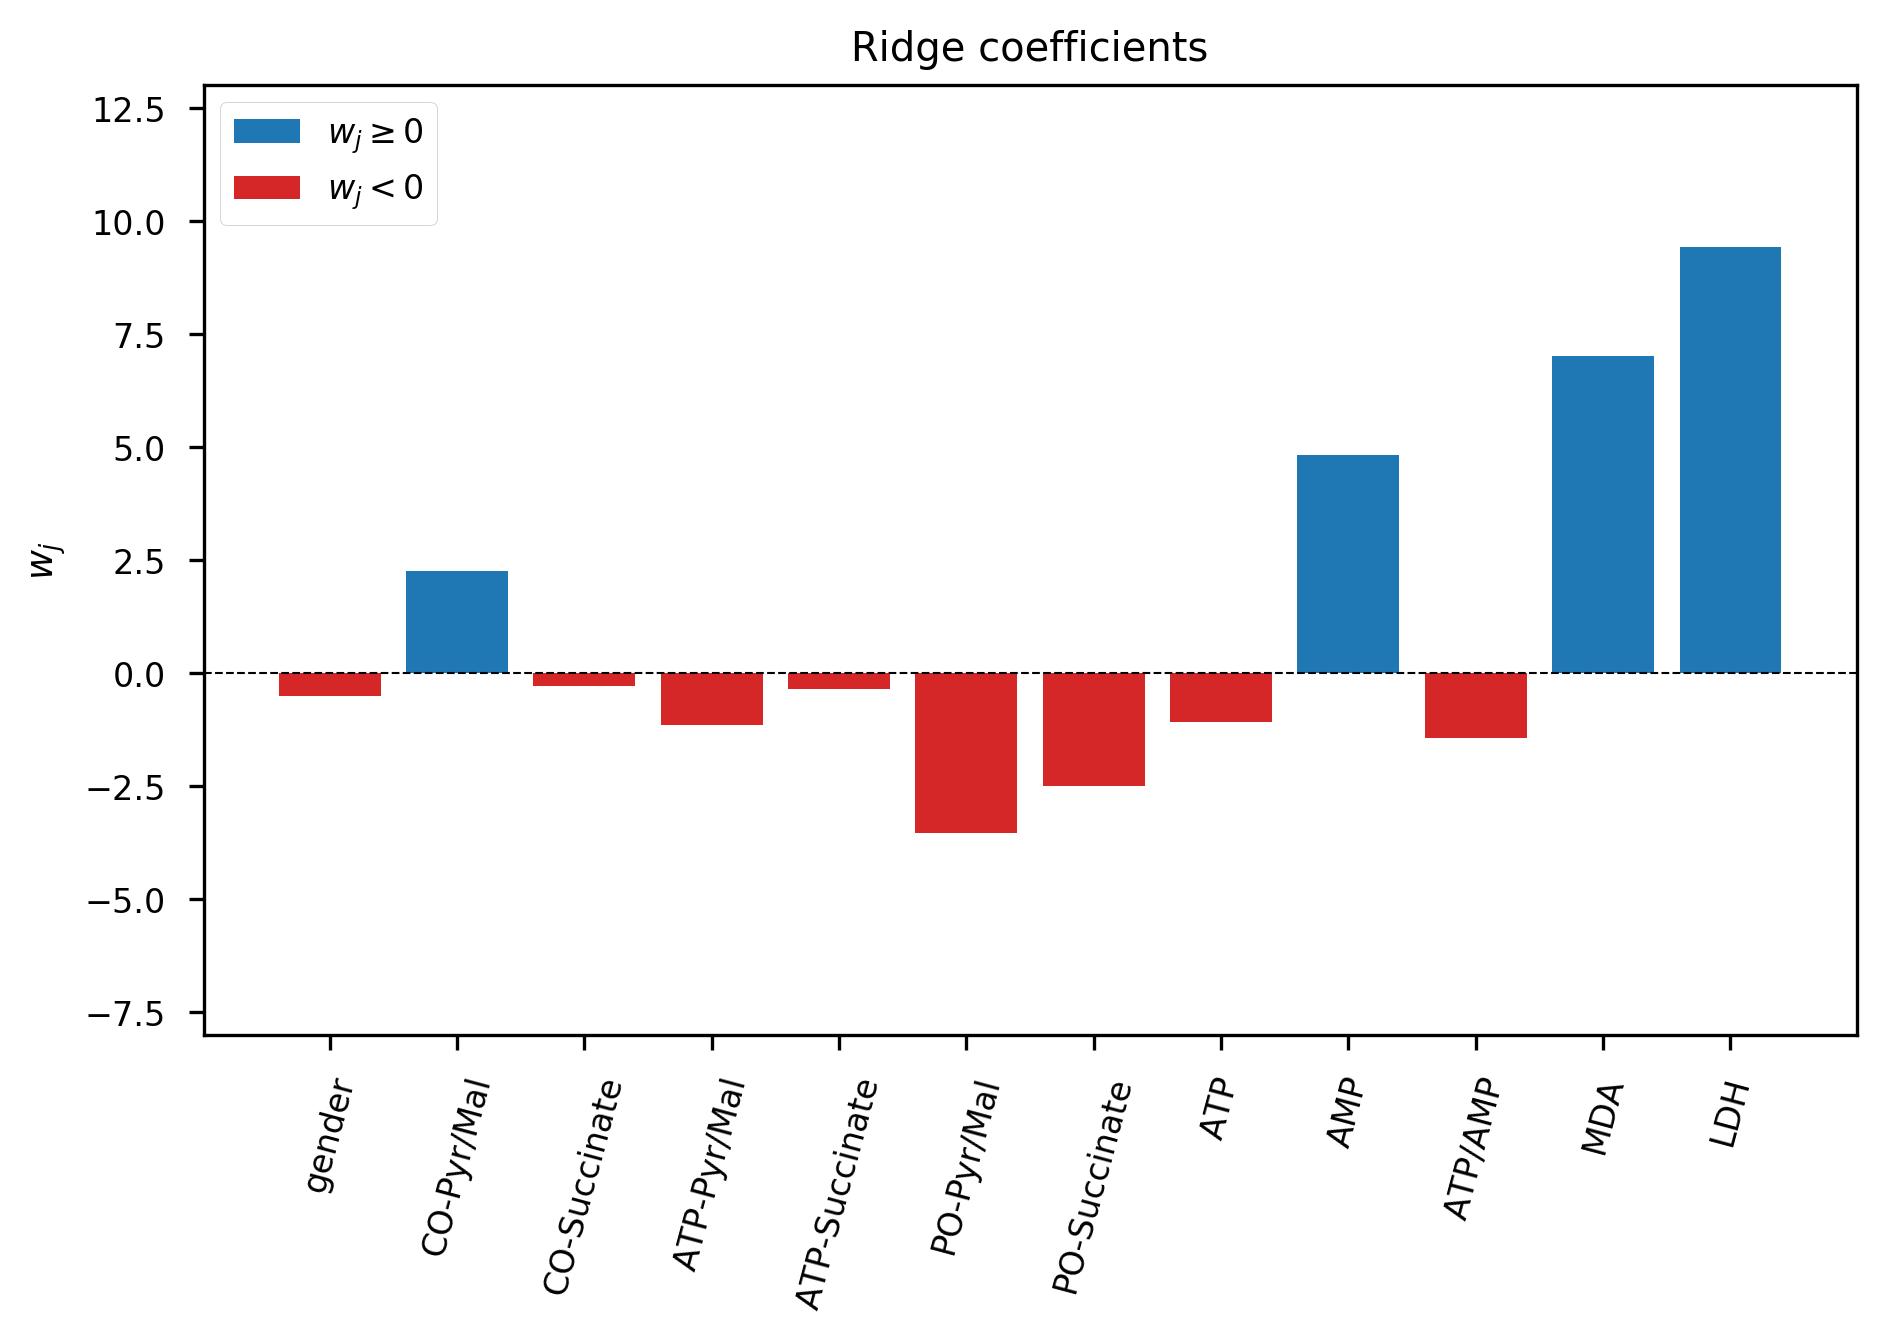
\includegraphics[width=0.8\textwidth]{part1/coefs_ridge.png}
				\caption{A pictorial representation of the vector $\bm{\hat w}_{\ell_2}$ obtained fitting a ridge regression model on $74$ randomly selected training samples of $\mathcal{D}_{\text{aging}}$. Variables associated with positive (\ie directly proportional to the output) and a negative (\ie inversely proportional) weight are represented in blue and red, respectively.} \label{fig:coefs_ridge}
			\end{figure}
			Comparing Figure~\ref{fig:coefs_ridge} and Figure~\ref{fig:coefs_ols} we can see that the amplitude of the ridge regression coefficients is, in absolute value, decreased by the use of the $\ell_2$ penalty. Indeed, several entries of $\bm{\hat w}_{\ell_2}$ are very small, but none of them is exactly zero. This is the expected behavior of the $\ell_2$-norm penalty. Evaluating $\bm{\hat w}_{\ell_2}$ on the test set, this model has  $\text{MAE}=8.615$ years and explains the $81.19\%$ of the variance, outperforming OLS.

			%%%%%%%%%%%%%%%%%%%%%%%%%%%%%%%%%%%%%%%
			\subsubsection{Lasso} \label{sec:the_lasso}
			%Tibshirani, in its seminal paper~\cite{tibshirani1996regression}, introduced the use of the $\ell_1$-norm  Equation~\eqref{eq:lasso}, as sparisty-enforcing regularizer for least squares problems.
			%In the original Lasso paper, the sparisty-enforcing properties of the $\ell_1$-norm, Equation~\eqref{eq:lasso}, as regularizer for least squares problems is typically known as the Lasso.
			%Such penalty is among the most popular sparsity-enforcing regularization method.

			The Lasso~\cite{tibshirani1996regression} can be defined as a least square problem penalized by the $\ell_1$-norm of the regression coefficients, see Equation~\eqref{eq:l1}.
			% In the Lasso, as in ridge regression (see Section~\ref{sec:ridge}), the data fidelity is measured by means of the square loss, while the $\ell_1$-norm, defined in Equation~\eqref{eq:lasso}, is used as regularization penalty.
			\begin{equation}\label{eq:l1}
				\mathcal{R}_{\mbox{$\ell_1$}}(\bm{w}) = \sum_{j=1}^d |w_j| = |\bm{w}|_1
			\end{equation}
			Therefore, the Lasso minimization problem can be written as in Equation~\eqref{eq:lasso}.

			\begin{equation} \label{eq:lasso}
				\bm{\hat w}_{\ell_1} = \argmin_{\bm{w} \in \mathbb{R}^d} \frac{1}{n} \sum_{i=1}^n (\bm{x}_i^T\bm{w} - y_i)^2 + \lambda  \sum_{j=1}^d |w_j| = \argmin_{\bm{w} \in \mathbb{R}^d} \frac{1}{n} \norm{X\bm{w} - \bm{y}}_2^2 + \lambda |\bm{w}|_1
			\end{equation}

			The Lasso can be used to perform linear model fitting and, thanks to its desirable properties, it is a popular choice for embedded variable selection~\cite{guyon2003introduction}, see Section~\ref{subsec:feature_selection}. At first, the $\ell_1$-norm enforces sparsity in the solution, hence producing compact and easily interpretable results. Secondly, the Lasso optimization problem is convex and, although non-differentiable, it is computationally feasible even in very high dimensional scenarios. Popular minimization algorithms for the Lasso problem are, for instance, the \textit{Fast Iterative Shrinkage-Thresholding Algorithm}  (\ac{FISTA})~\cite{beck2009fast} and the \textit{coordinate descent algorithm}~\cite{wu2008coordinate}. A pictorial representation of the Lasso solution can be seen in Figure~\ref{fig:w_lasso}.

			A popular application of the Lasso is to perform shrinkage and variable selection in survival analysis for Cox proportional hazard regression \cite{tang2017spike, gui2005penalized, tibshirani1997lasso} and additive risk models~\cite{ma2007additive}.
			Such $\ell_1$-penalized methods are extensively applied in literature to predict survival time from molecular data collected from patients affected by different kinds of tumor.
			%\todo{Add use cases: lu2011lasso, rakitsch2013lasso $\dots$}

			The Lasso can also be extended to vector-valued regression problems by using the mixed $L_{2,1}$-norm, defined in Equation~\eqref{eq:L21}, as regularization penalty~\cite{gramfort2012mixed}.
			\begin{equation}\label{eq:L21}
				\mathcal{R}_{\ell_1}(W)= \sum_{j=1}^d\sqrt{\Bigg(\sum_{t=1}^k |w_j^t|^2\Bigg)} = \norm{W}_{2,1}
			\end{equation}
			Therefore, the vector-valued regularization problem can be written as in Equation~\eqref{eq:multitask_lasso}
			\begin{equation} \label{eq:multitask_lasso}
				\begin{aligned}
					\hat W_{\ell_1}={} & \argmin_{W \in \mathbb{R}^{d \times k}} \frac{1}{n} \sum_{i=1}^n \sum_{t=1}^k (\bm{x}_i^T\bm{w}^t - y_i^t)^2 + \lambda  \sum_{j=1}^d \sqrt{\Bigg(\sum_{t=1}^k |w_j^t|^2\Bigg)} \\
					& =	\argmin_{W \in \mathbb{R}^{d \times k}} \frac{1}{n} \norm{XW - Y}_F^2 + \lambda ||W||_{2,1}
				\end{aligned}
			\end{equation}
			and it is known as Multi-task Lasso~\cite{lee2010adaptive}. Such norm enforces a row-structured sparsity in the regression weights, hence preserving the interpretability of the solution.

			Originally proposed to solve regression problems, the Lasso can also be adopted in binary classification tasks; although, in this case, \textit{sparse logistic regression} (see Section~\eqref{sec:logistic_regression}) is often preferred~\cite{tong2009genome}.

			Let's see what happens when the Lasso model is applied to a real regression problem. Once again, for ease of comparison with OLS and ridge, we take into account the dataset $\mathcal{D}_{\text{aging}}$, introduced in Section~\ref{sec:ols}. The experimental setup in this case is identical to the one previously applied for ridge regression. The best value for the regularization parameter, chosen via grid-search cross-valudation, is $\hat \lambda_{\text{cv}}=1.27$. The Lasso coefficients $\bm{ \hat w}_{\ell_1}$ are represented in Figure~\ref{fig:coefs_lasso}.
			\begin{figure}[!h]
				\centering
				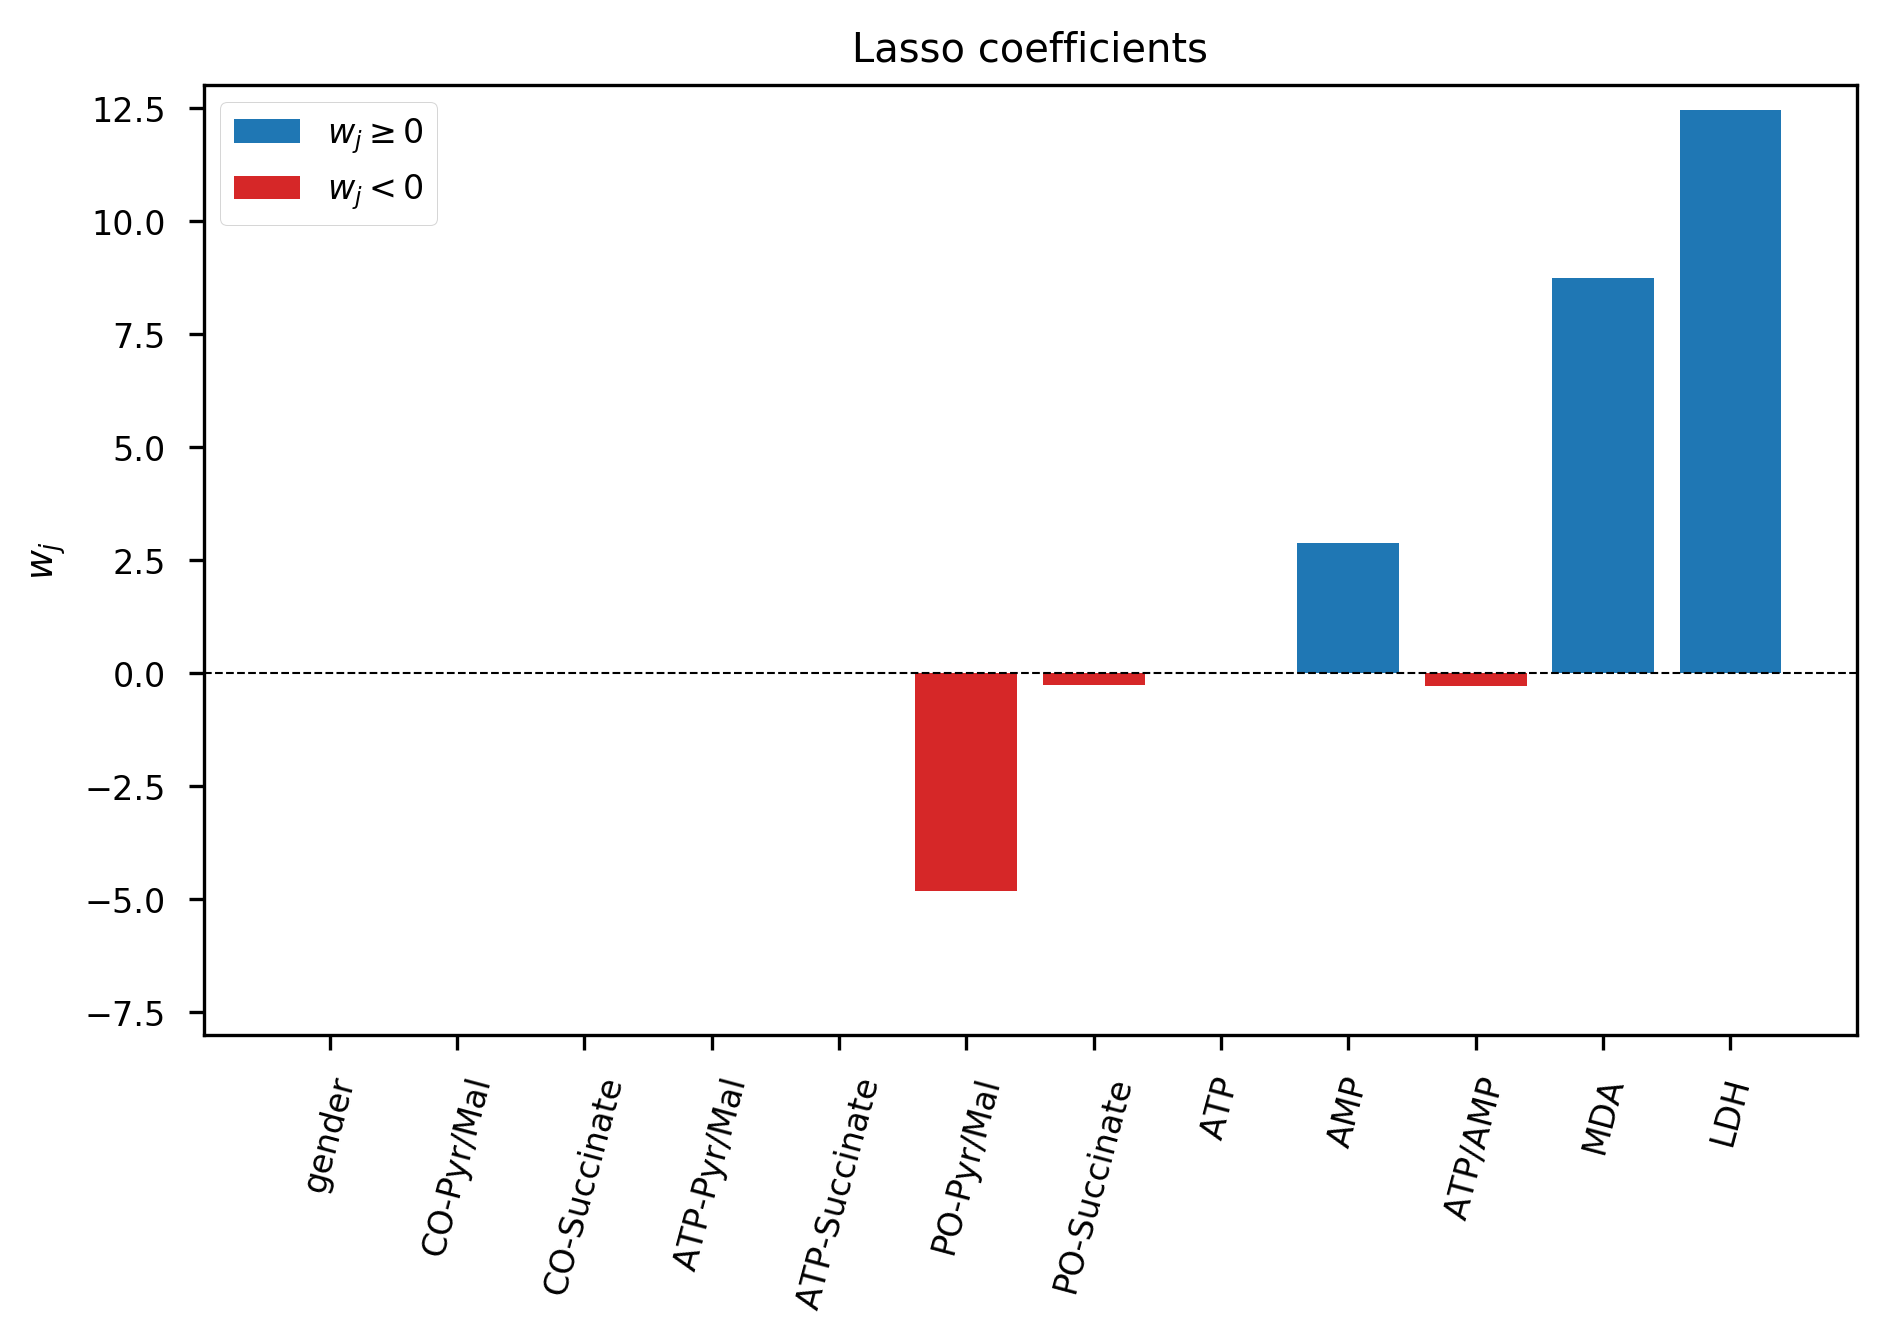
\includegraphics[width=0.8\textwidth]{part1/coefs_lasso.png}
				\caption{A pictorial representation of the vector $\bm{\hat w}_{\ell_1}$ obtained fitting a Ridge model on $74$ randomly selected training samples of $\mathcal{D}_{\text{aging}}$. Variables associated with positive (\ie directly proportional to the output) and a negative (\ie inversely proportional) weight are represented in blue and red, respectively.} \label{fig:coefs_lasso}
			\end{figure}
			Comparing $\bm{\hat w}_{\ell_1}$ with $\bm{\hat w}_{\ell_2}$ and $\bm{\hat w}_{\text{OLS}}$ (Figure~\ref{fig:coefs_lasso}, Figure~\ref{fig:coefs_ridge} and Figure~\ref{fig:coefs_ols}, respectively) we can observe that, for the first time, to only $6$ variables, out of $12$, a non-negative value is assigned. This is an example of the \textit{sparsity}-enforcing effect of the $\ell_1$-norm regularization penalty.
			The $6$ variables with nonzero weight can be considered as \textit{selected} for the prediction problem at hand.
			Evaluating $\bm{\hat w}_{\ell_1}$ on the test set, the Lasso has  $\text{MAE}=8.387$ years and explains the $81.51\%$ of the variance, slightly outperforming ridge.

			Using sparsity-enforcing penalties, such as the $\ell_1$-norm, an insightful experiment is the analysis of the regularization path. This can be done by iteratively fitting the model with decreasing values of the regularization parameter $\lambda$, usually expressed in logarithmic scale. An example of the Lasso path for the aging problem is reported in Figure~\ref{fig:lasso_path}.
			\begin{figure}[!h]
				\centering
				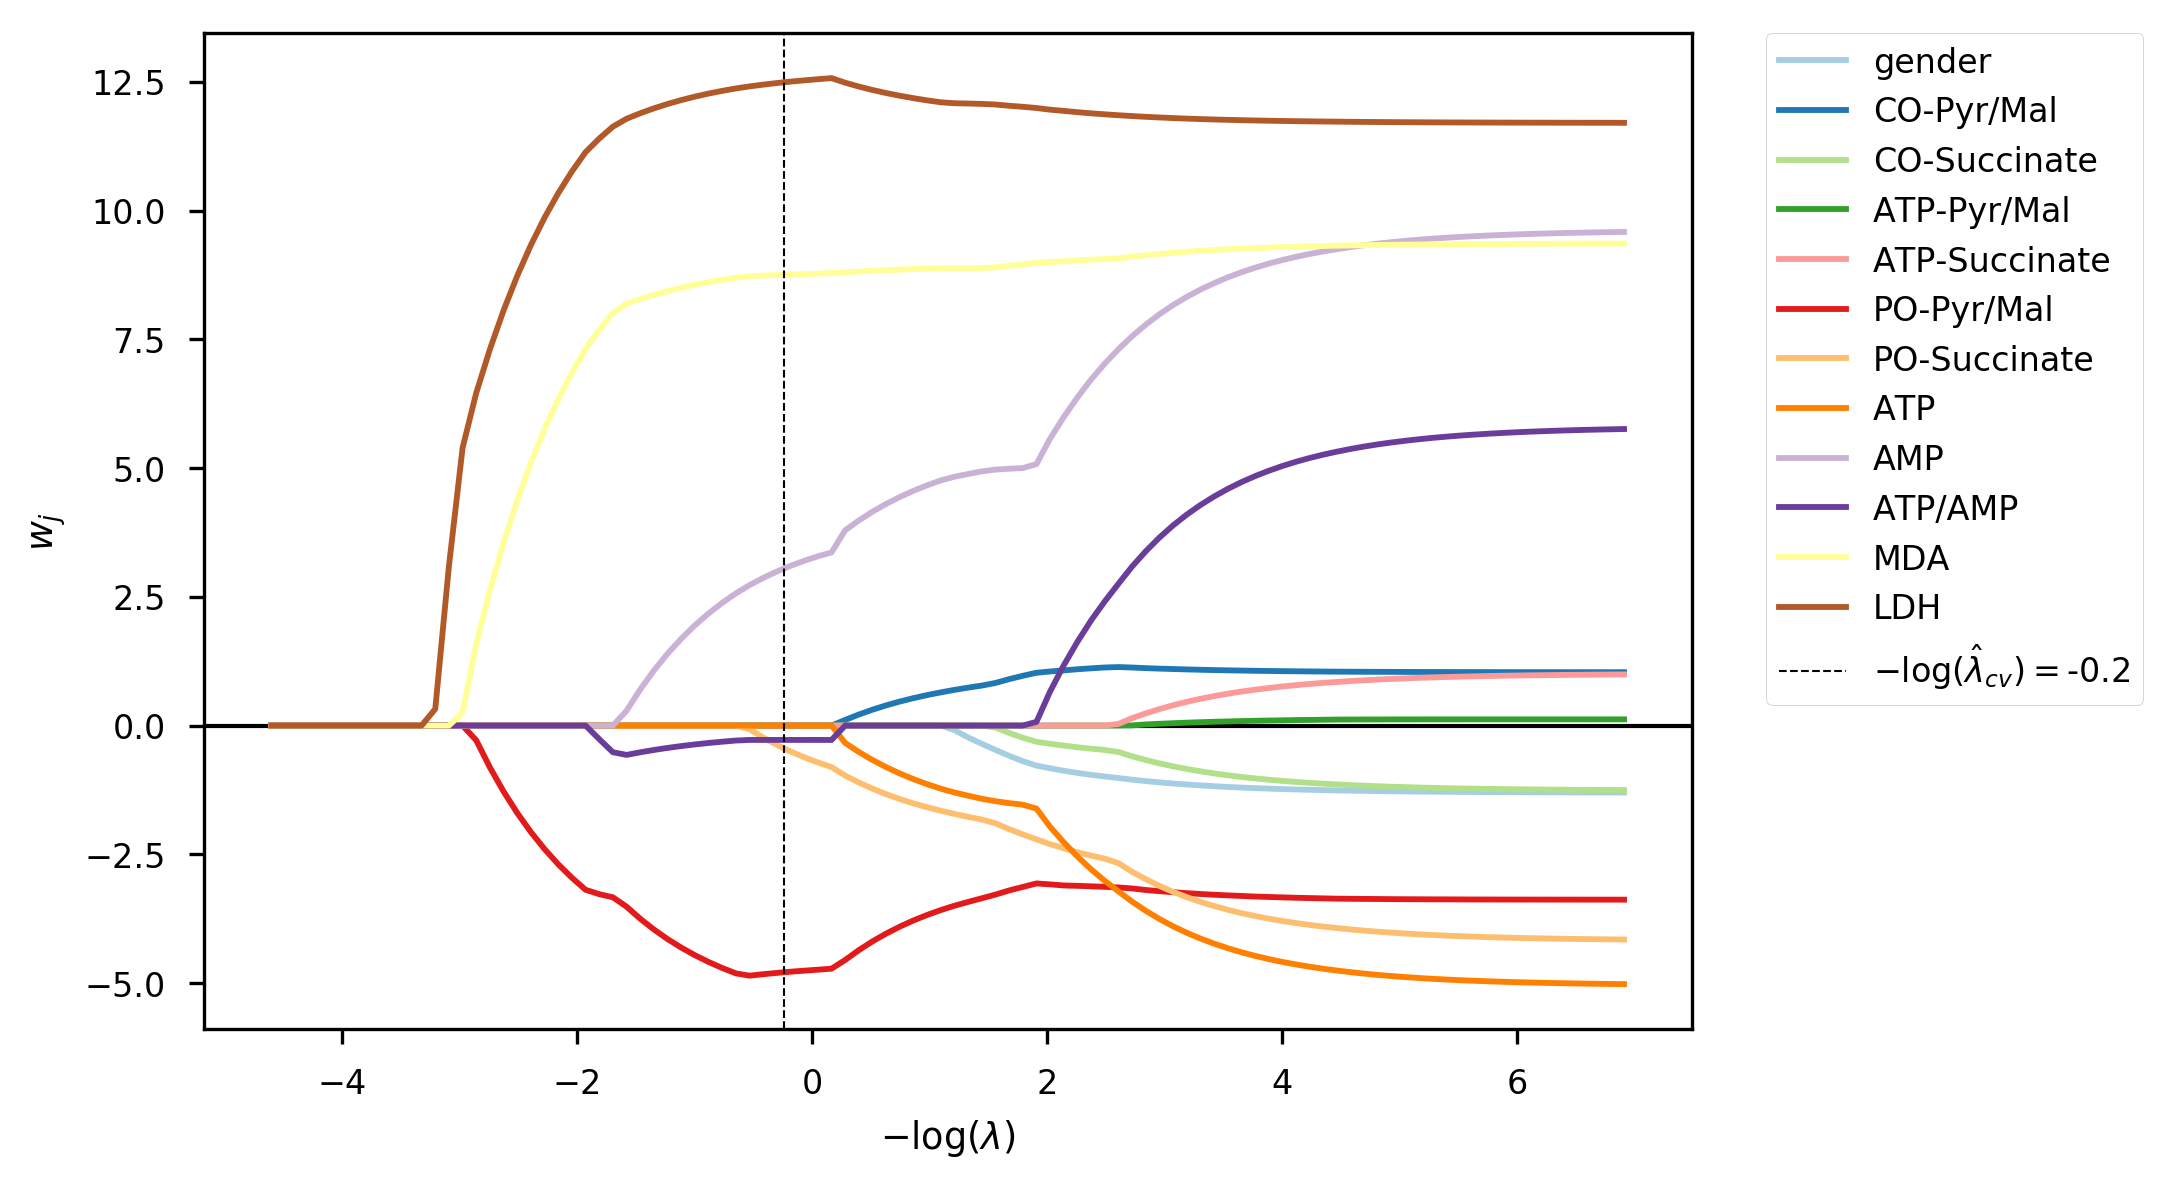
\includegraphics[width=0.8\textwidth]{part1/lasso_path.png}
				\caption{Profiles of the Lasso coefficients for the aging problem as $\lambda$ decreases. The vertical dashed line represents the optimal value $\hat \lambda_{\text{cv}}$ estimated by grid-search ($5$-fold) cross-validation.} \label{fig:lasso_path}
			\end{figure}
			Weights corresponding to features that are more likely to be relevant for the prediction problem should early move away from the horizontal axis. Conversely, as the regularization parameter increases, the model should enforce less sparsity, hence tolerating more and more irrelevant features having nonzero weight. The vertical dashed line in Figure~\ref{fig:lasso_path} corresponds to $\hat \lambda_{\text{cv}}$ and it hits the profiles of the weights consistently with what shown in Figure~\ref{fig:coefs_lasso}.

			When used for variable selection, the Lasso has two major drawbacks. First, in presence of groups of correlated variables, this method tends to select only one variable per group, ignoring the others. Secondly, the method cannot select more variables than the sample size~\cite{waldmann2013evaluation, de2009regularized}.
			The effect of such drawbacks is dramatic when using the Lasso in $n \ll d$ scenarios.
			In order to ameliorate this issues, several Lasso-inspired models were proposed~\cite{meinshausen2010stability, hoggart2008simultaneous, zou2006adaptive}.
			% (see Section~\ref{sec:other_sparsity}).
			In the next section we will describe one of the most popular and straightforward Lasso extensions: the Elastic-Net~\cite{zou2005regularization}.

			%%%%%%%%%%%%%%%%%%%%%%%%%%%%%%%%%%%%%%%
			\subsubsection{Elastic-Net} \label{sec:elastic_net}
			The Elastic-Net~\cite{zou2005regularization, de2009elastic} method can be formulated as a least squares problem penalized by a convex combination of Lasso ($\ell_1$-norm) and ridge regression ($\ell_2$-norm) penalties, as in Equation~\eqref{eq:l1l2}.

			\begin{equation}\label{eq:l1l2}
				R_{\mbox{$\ell_1\ell_2$}}(\bm{w}) = \sum_{j=1}^d (\alpha\,|w_j| + (1-\alpha)\,w_j^2) = \alpha\,|\bm{w}|_1 + (1-\alpha)\,\norm{\bm{w}}_2^2
			\end{equation}

			Therefore, the Elastic-Net minimization problem can be written as in Equation~\eqref{eq:enet}
			\begin{equation} \label{eq:enet}
				\begin{aligned}
				\bm{\hat w}_{\ell_1\ell_2} = {} & \argmin_{\bm{w} \in \mathbb{R}^d} \frac{1}{n} \sum_{i=1}^n (\bm{x}_i^T\bm{w} - y_i)^2 + \lambda\,\bigg[ \sum_{j=1}^d (\alpha\,|w_j| + (1-\alpha)\,w_j^2) \bigg] \\
				& = \argmin_{\bm{w} \in \mathbb{R}^d} \frac{1}{n} \norm{X\bm{w} - \bm{y}}_2^2 + \lambda\,\big[ \alpha\,|\bm{w}|_1 + (1-\alpha)\,\norm{\bm{w}}_2^2 \big]
			\end{aligned}
		  \end{equation}
			with $0 \leq \alpha \leq 1$, or equivalently as
			\begin{equation} \label{eq:enet_l1l2}
			\bm{\hat w}_{\ell_1\ell_2} = \argmin_{\bm{w} \in \mathbb{R}^d} \frac{1}{n} \norm{X\bm{w} - \bm{y}}_2^2 + \tau\,|\bm{w}|_1 + \mu\,\norm{\bm{w}}_2^2
			\end{equation}
			where $\tau = \lambda\alpha$ and $\mu = \lambda(1-\alpha)$. The first formulation of the problem, Equation~\eqref{eq:enet}, is more convenient when we want to control the overall amount of regularization with $\lambda$, given a certain amount of sparsity $\alpha$. In fact, it is easy to see that fitting the Elastic-Net model for $\alpha=0$ or $\alpha=1$ is equivalent to solve ridge or Lasso regression, respectively. On the other hand, writing the Elastic-Net problem as in Equation~\eqref{eq:enet_l1l2} is more convenient when we want to separately control the $\ell_1$- and $\ell_2$-norm penalties, as in~\cite{de2009regularized}.

			The Elastic-Net\footnote{actually, in the original paper the authors refer to Equations~\eqref{eq:enet} and~\eqref{eq:enet_l1l2} as \textit{na\"ive} Elastic-Net~\cite{zou2005regularization} because empirical evidence show that the weights $\bm{\hat w}_{\ell_1\ell_2}$ may suffer from over-shrinking when appropriate rescaling strategies, also described in~\cite{de2009regularized},  are not applied.} model is widely adopted to perform linear model fitting and variable selection. Indeed, the combined presence of the two norms promotes sparse solutions were groups of correlated variables can be simultaneously selected, hence overcoming the variable selection drawbacks of the Lasso and making the Elastic-Net suitable for variable selection in $n \ll d$ scenarios.
			As already seen for the Lasso, the minimization problem in Equation~\eqref{eq:enet} is convex and non-differentiable, due to the $\ell_1$-norm, and it can be efficiently solved either by proximal forward-backward splitting strategies (\eg FISTA~\cite{beck2009fast}), or by coordinate descent~\cite{wu2008coordinate}. A pictorial representation of the Elastic-Net solution can be seen in Figure~\ref{fig:w_enet}.

			The Elastic-Net method is successfully applied in several biomedical fields, including gene expression~\cite{jacob2015robust, de2009regularized}, genome-wide association studies~\cite{waldmann2013evaluation} and other molecular data~\cite{aben2016tandem, jacob2015robust}.
			% In~\cite{csala2017sparse} the authors propose an iterative algorithm that exploits the variable selection capabilities of this method to estimate explanatory variables weights  in sparse redundancy analysis; such method is applied to explain the variability in gene expressions by epigenomic data (\ie methylation markers) collected from blood leukocytes of Marfan Syndrome patients.


			The Elastic-Net can also be extended to vector-valued regression problems by using a convex combination of the $L_{2,1}$- and the Frobenius norms. This multiple output regression problem is known as Multi-task Elastic-Net~\cite{chen2012adaptive} can be written as in Equation~\eqref{eq:multitask_enet}.
			\begin{equation} \label{eq:multitask_enet}
				\begin{aligned}
					\hat W_{\ell_1\ell_2}={} & \argmin_{W \in \mathbb{R}^{d \times k}} \frac{1}{n} \sum_{i=1}^n \sum_{t=1}^k (\bm{x}_i^T\bm{w}^t - y_i^t)^2 + \lambda \bigg[ \alpha \sum_{j=1}^d \sqrt{\Bigg(\sum_{t=1}^k |w_j^t|^2\Bigg)} + (1-\alpha)  \sum_{j=1}^d \sum_{t=1}^k |w_j^t|^2 \bigg] \\
					& =	\argmin_{W \in \mathbb{R}^{d \times k}} \frac{1}{n} \norm{XW - Y}_F^2 + \lambda [\alpha\,||W||_{2,1} + (1-\alpha)\,\norm{W}_F^2]
				\end{aligned}
   		\end{equation}

			Even though originally proposed to solve regression problems, as already seen for Lasso and ridge regression, the Elastic-Net can be adopted in binary classification tasks. Nevertheless, for classification problems, the use of the logistic loss is usually preferred.

			Let's see what happens when the Elastic-Net model is applied to an actual regression problem. As usually, we tackle the aging task (introduced in Section~\ref{sec:ols}).
			The experimental setup in this case is the same already adopted for the Lasso in Section~\ref{sec:the_lasso}. The only difference is that the grid-search cross-validation routine looks for the optimal values for the two regularization parameters $(\hat \lambda_{\text{cv}}, \hat \alpha_{\text{cv}}) = (0.57, 0.48)$ in a 2D grid consisting of $30 \times 30$ values ($\alpha$ candidates range from $0$ to $1$ in a linear scale, whilst $\lambda$ candidates range from $10^{-3}$ to $10^{2}$ in a logarithmic scale). The Elastic-Net coefficients $\bm{\hat w}_{\ell_1\ell_2}$ are represented in Figure~\ref{fig:coefs_enet}.

			\begin{figure}[!h]
				\centering
				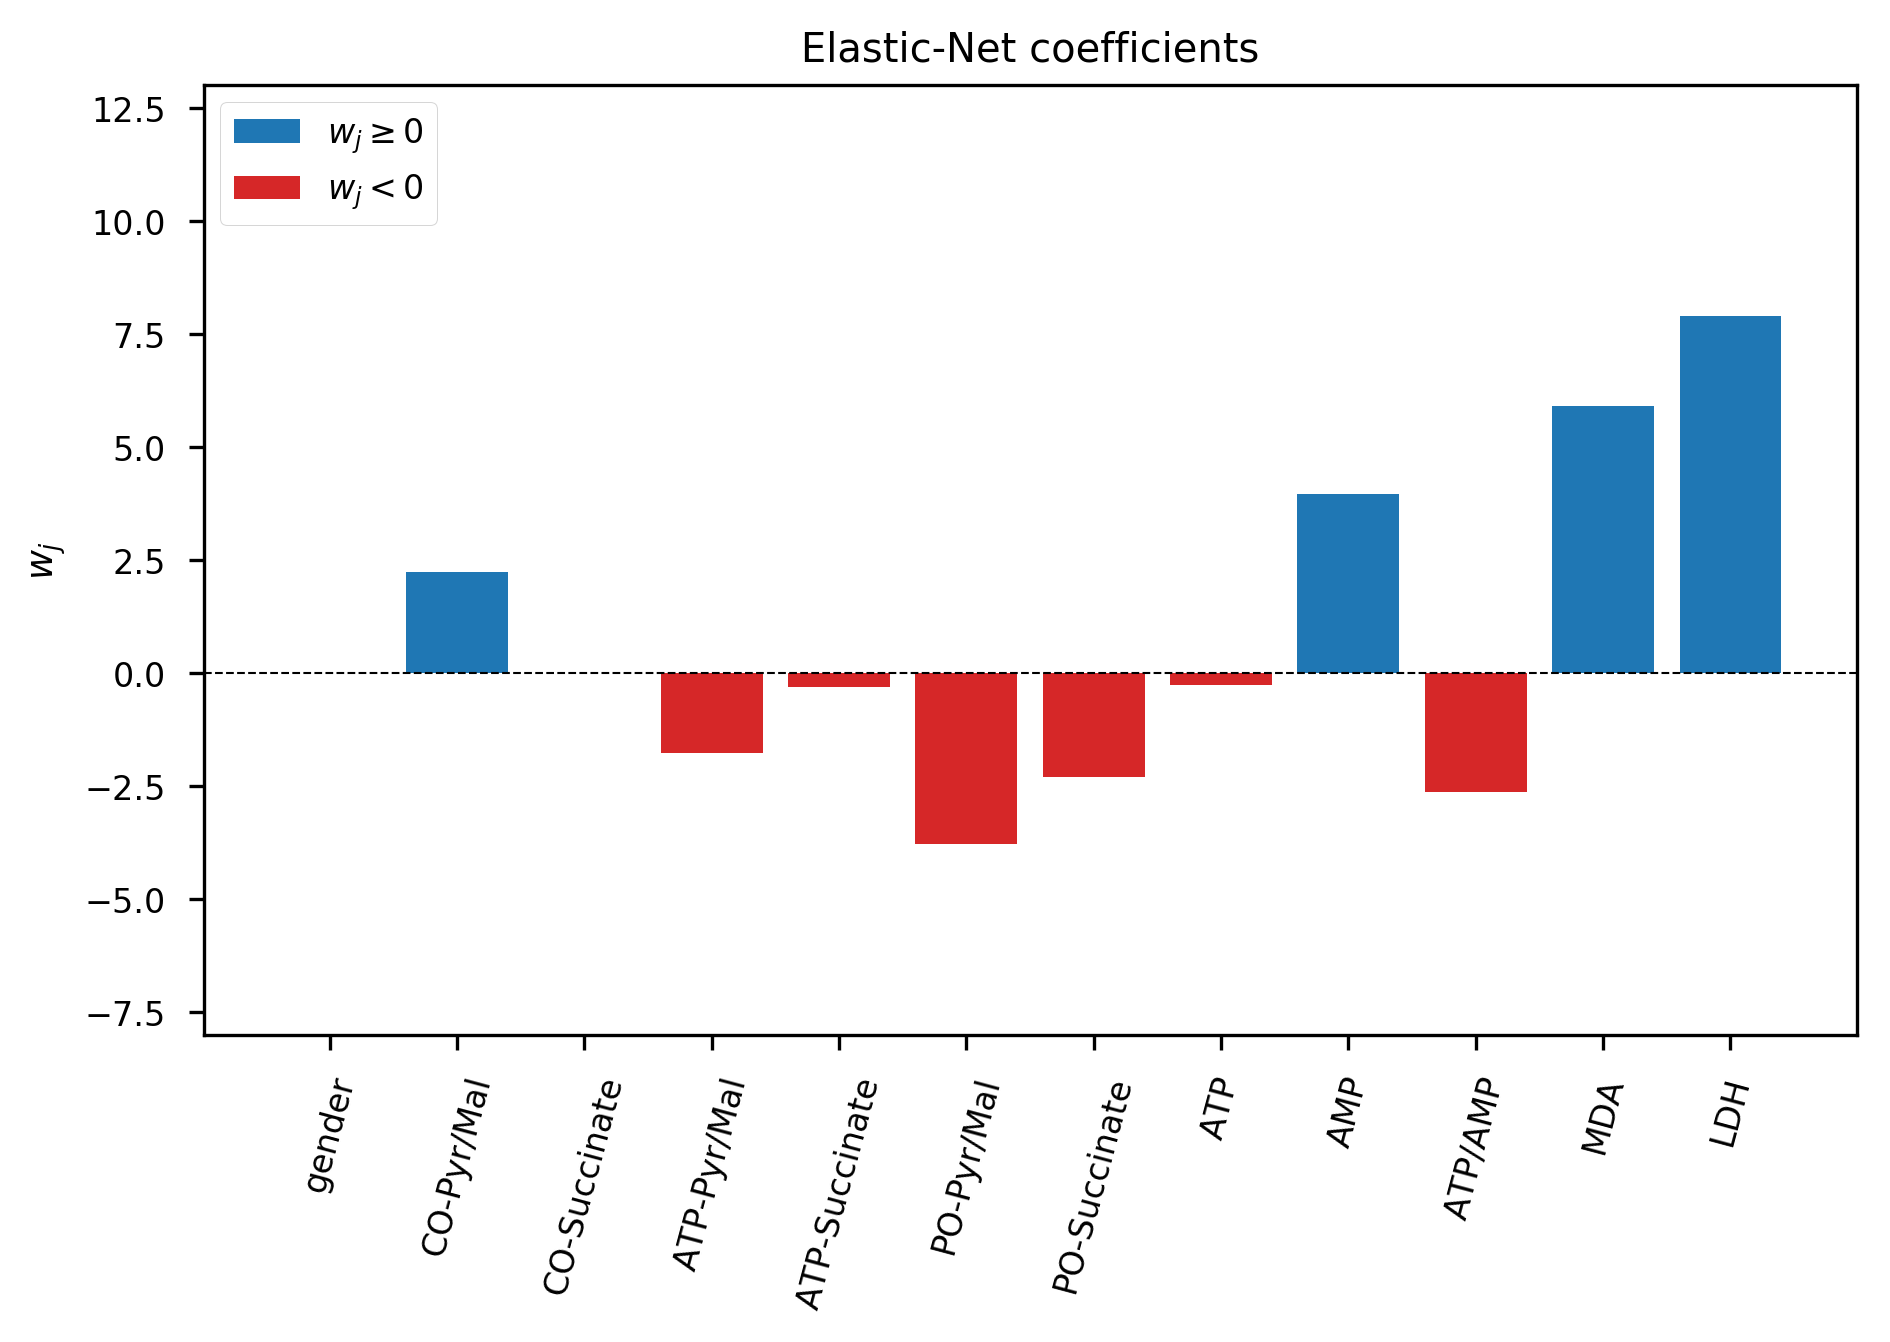
\includegraphics[width=0.8\textwidth]{part1/coefs_enet.png}
				\caption{A pictorial representation of the vector $\bm{\hat w}_{\ell_1\ell_2}$ obtained fitting a Elastic-Net model on $74$ randomly selected training samples of $\mathcal{D}_{\text{aging}}$. Variables associated with positive (\ie directly proportional to the output) and a negative (\ie inversely proportional) weight are represented in blue and red, respectively.} \label{fig:coefs_enet}
		  \end{figure}

			Comparing $\bm{\hat w}_{\ell_1\ell_2}$ in Figure~\ref{fig:coefs_enet} with $\bm{\hat w}_{\ell_1}$ in Figure~\ref{fig:coefs_lasso} we can notice that in the Elastic-Net solution $10$ variables have nonzero weight, that is more with respect to the $6$ of the Lasso. This is the expected behavior of the added $\ell_2$-norm, which helps the model to select groups of collinear variables. Evaluating the Elastic-Net solution on the test set, $\bm{\hat w}_{\ell_1\ell_2}$ achieves $\text{MAE} = 8.321$ years explaining the $82.13\%$, slightly outperforming Lasso, hence ranking first in this little challenge of linear square loss-based regression methods.

			As already seen for the Lasso, we can inspect the Elastic-Net weights path, obtained fixing $\alpha = \hat \alpha_{\text{cv}}$ for decreasing values of $\lambda$, see Figure~\ref{fig:enet_path}.
			\begin{figure}[!h]
				\centering
				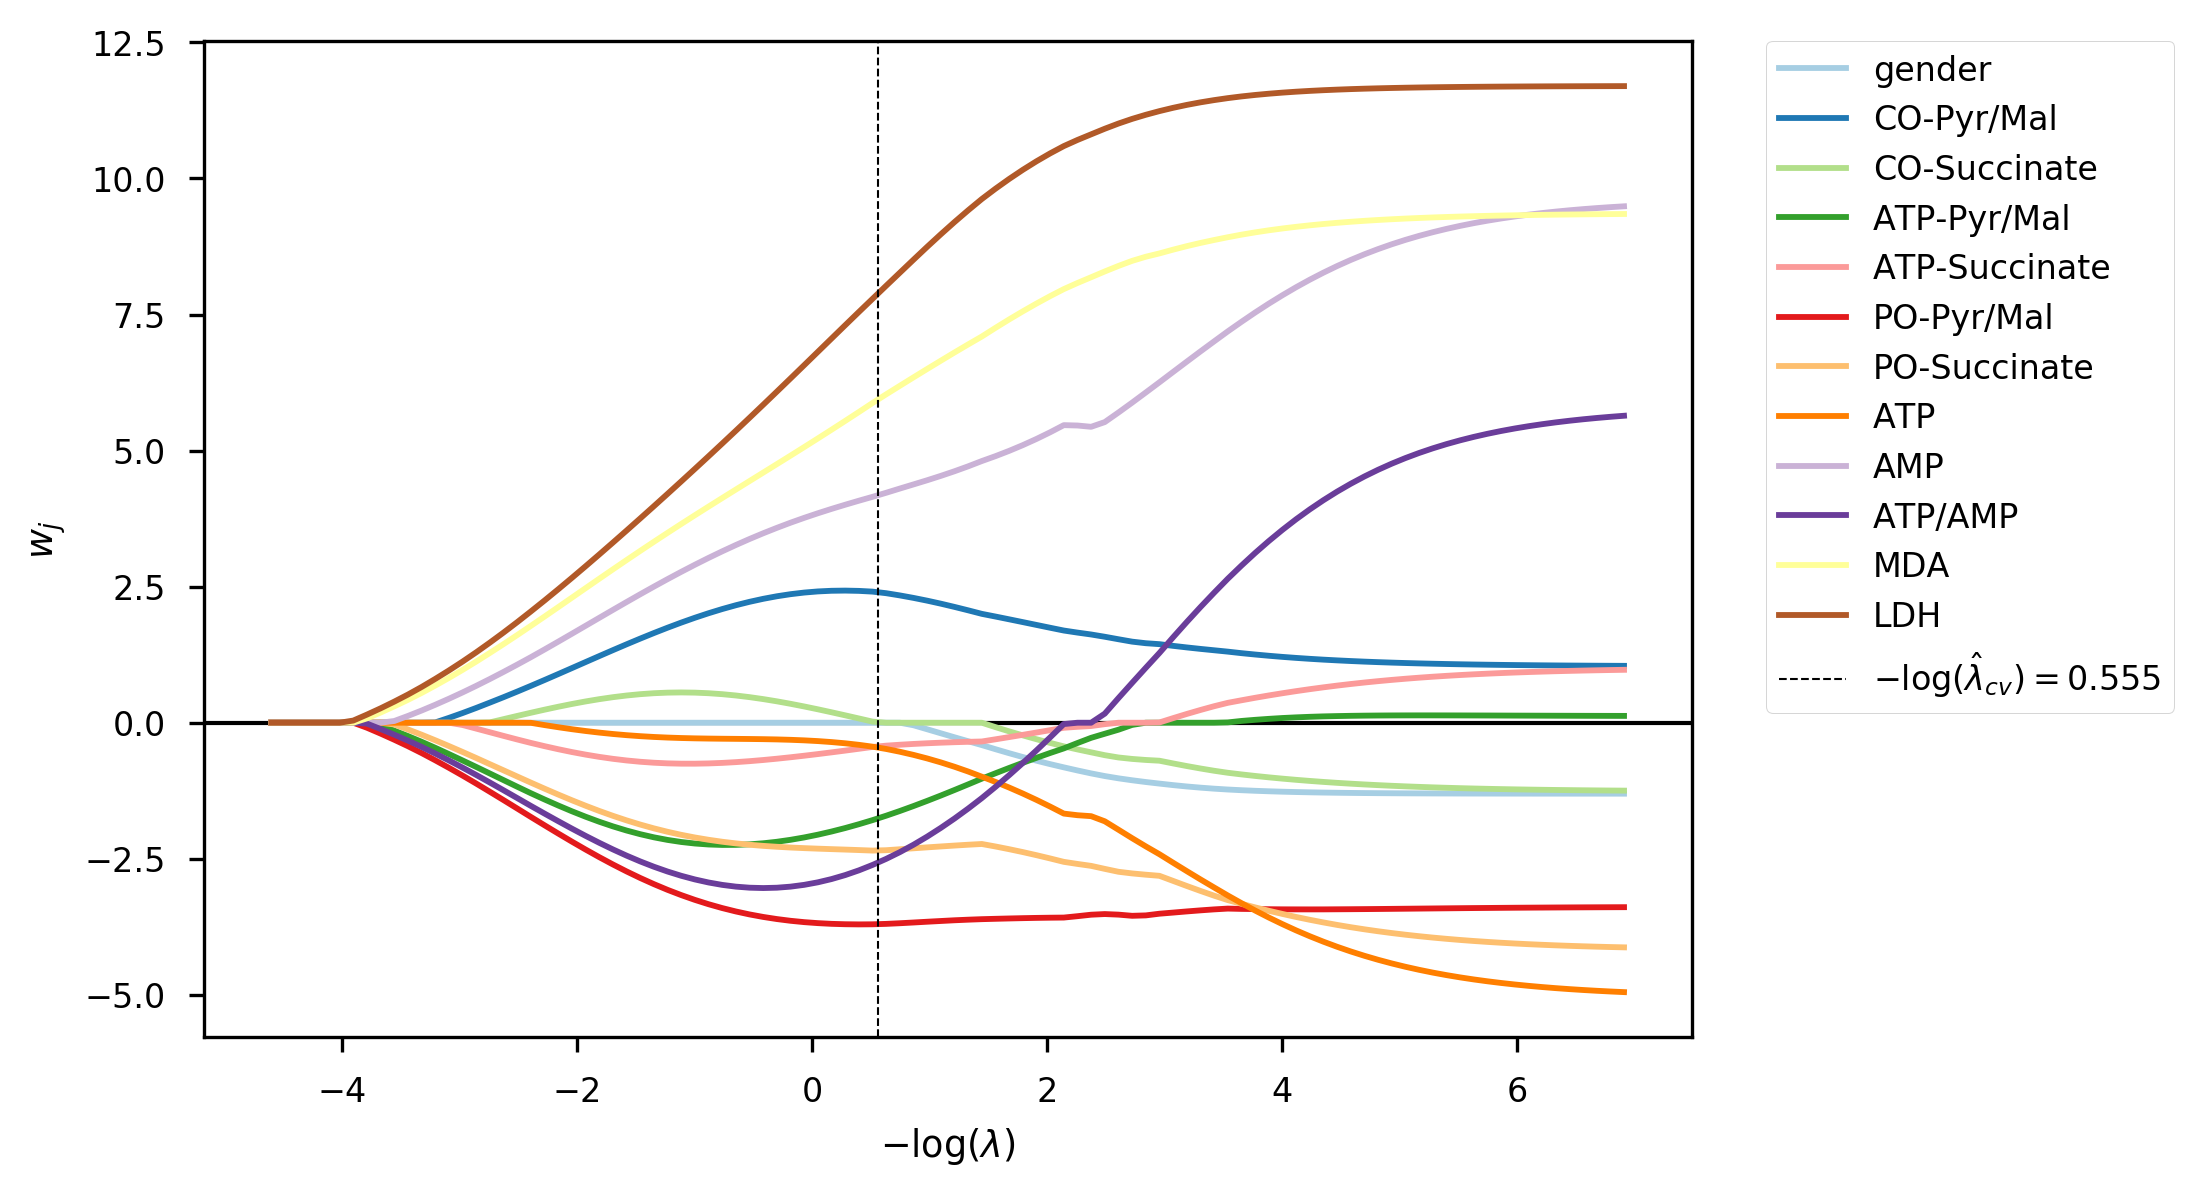
\includegraphics[width=0.8\textwidth]{part1/enet_path.png}
				\caption{Profiles of the Elastic-Net coefficients for the aging problem as $\lambda$ decreases. The vertical dashed line represents the optimal value $\hat \lambda_{\text{cv}}$ estimated by grid-search ($5$-fold) cross-validation.} \label{fig:enet_path}
			\end{figure}
			The vertical dashed line in Figure~\ref{fig:enet_path} corresponds to $\hat \lambda_{\text{cv}}$ and it hits the profiles of the weights consistently with the Elastic-Net solution represented in Figure~\ref{fig:coefs_lasso}. The Elastic-Net, compared to the Lasso, produces smoother regularization paths in which the allegedly correlated variables enter the solution earlier.

			Another comparison between the behavior of OLS, ridge, Lasso and Elastic-Net regression is presented in Figure~\ref{fig:l1l2_norms_scatterplot}. The four solutions achieved for the same aging regression problem are represented in a scatter plot where horizontal and vertical axis represents their $\ell_2$- and $\ell_1$-norm, respectively.
			\begin{figure}[!h]
				\centering
				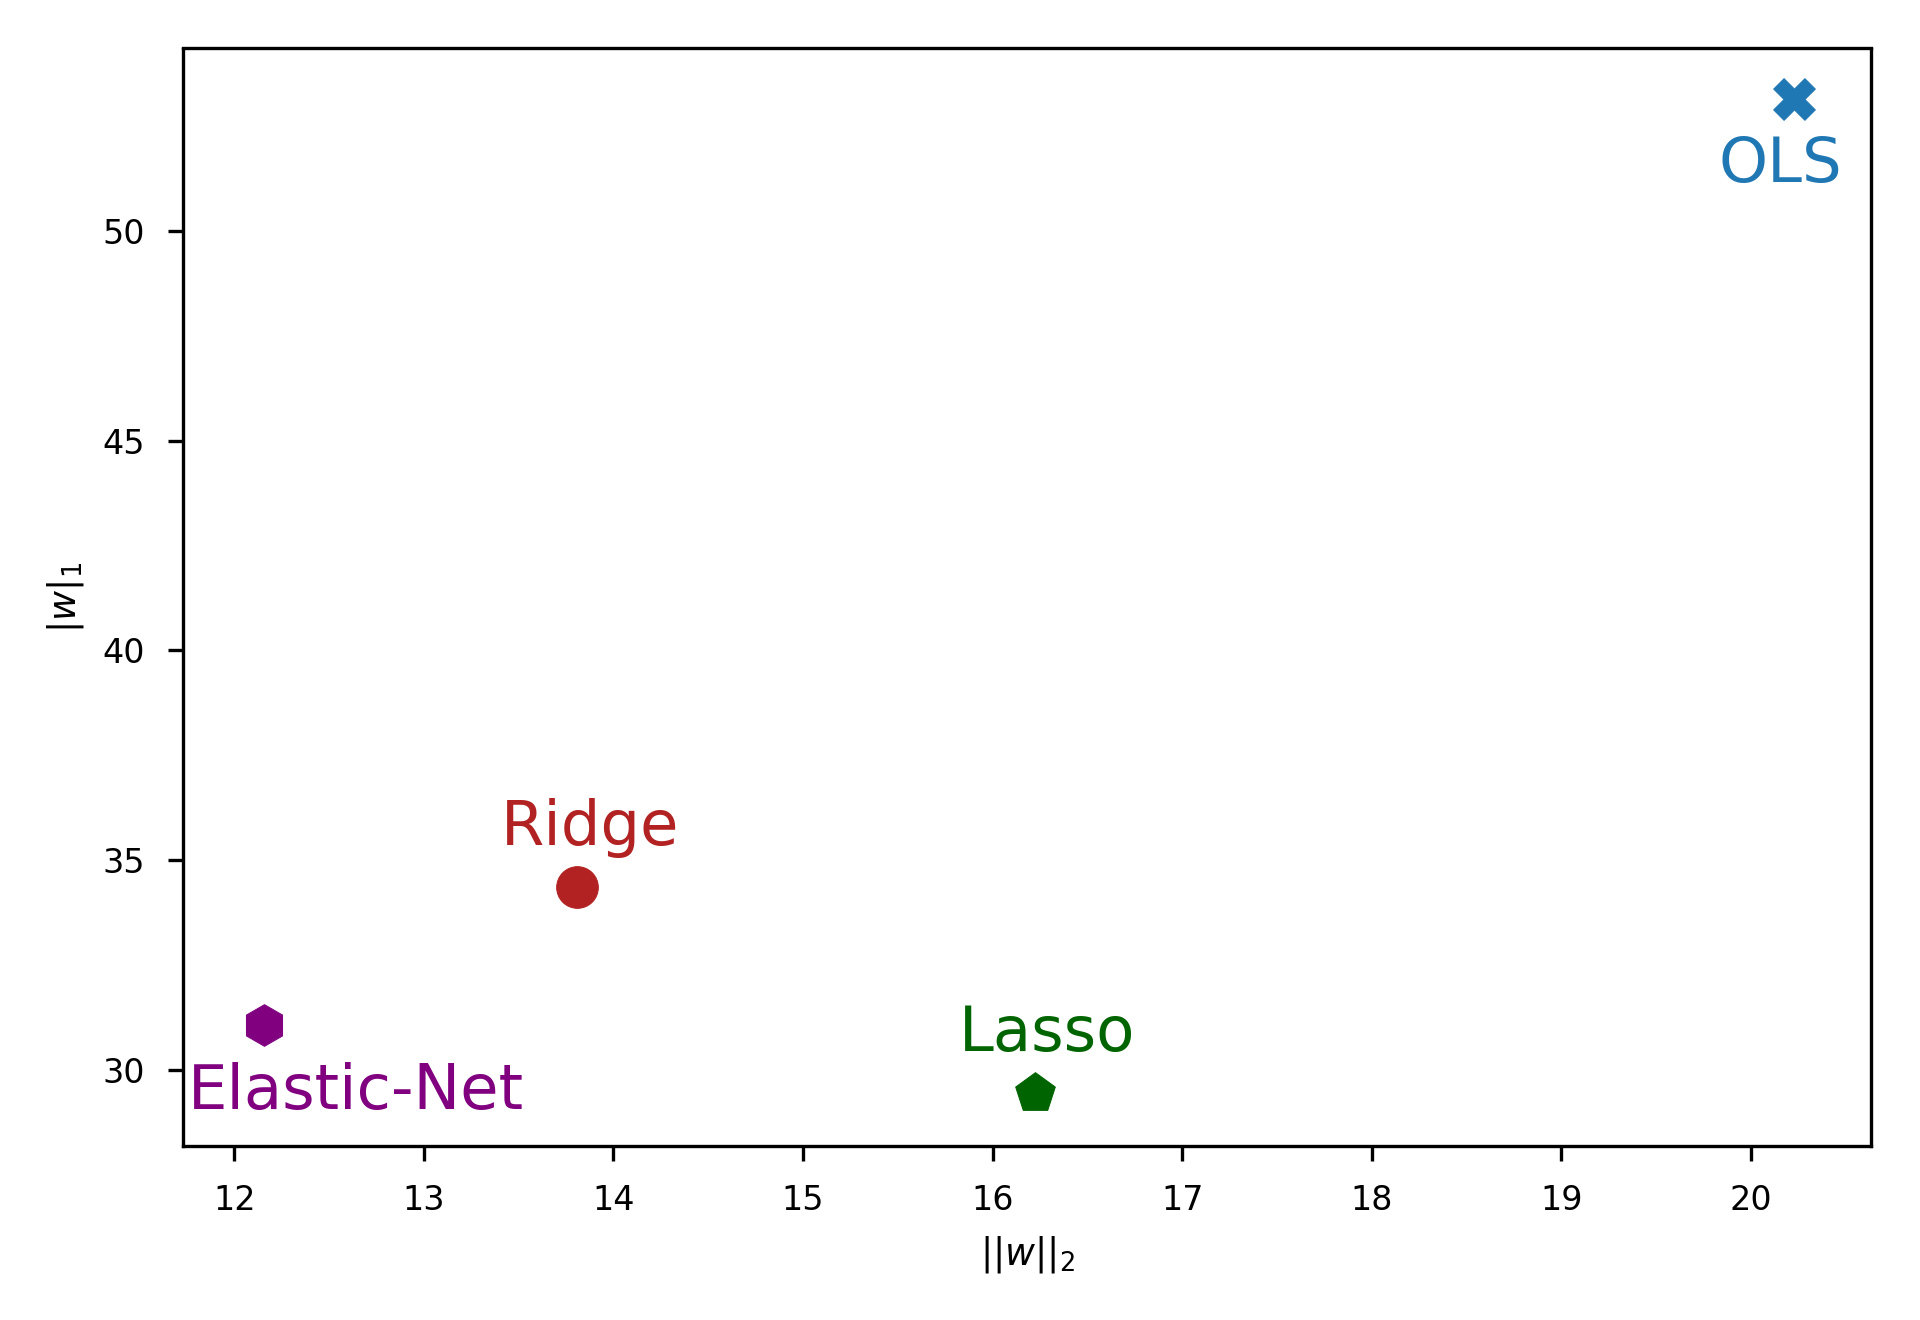
\includegraphics[width=0.8\textwidth]{part1/l1l2_norms_scatterplot.png}
				\caption{A comparison of the value of the $\ell_1$ and $\ell_2$ norms of the weights obtained by OLS, ridge, Lasso and Elastic-Net.} \label{fig:l1l2_norms_scatterplot}
		  \end{figure}
			As expected,
			\begin{enumerate}
				\item the unpenalized solution $\bm{\hat w}_{\text{OLS}}$ shows the highest values for the two norms and it is placed in the top-right side of the plot,
				\item the ridge solution $\bm{\hat w}_{\ell_2}$ has lowest $\ell_2$-norm,
				\item the Lasso solution $\bm{\hat w}_{\ell_1}$ has lowest $\ell_1$-norm and
				\item the Elastic-Net solution shows the lowest values for the two norms and it is placed in the bottom-left side of the plot.
		  \end{enumerate}
			This is consistent with the type of regularization imposed to each method. Interestingly, in this case, the method that performs better on the test set (Elastic-Net) has lowest norms.

			The Elastic-Net penalty is not the only method in which sparsity is enforced on a group level. For example, (overlapping) group Lasso and graph Lasso penalties can be applied when the variables are naturally partitioned in (overlapping) groups, or when their interaction can be modeled by a graph. A detailed description of these methods is beyond the scope of this thesis and we refer to~\cite{jacob2009group, witten2009covariance} and references therein for their comprehensive description.

			\begin{figure}[]
				\centering
				\subfloat[]{%
					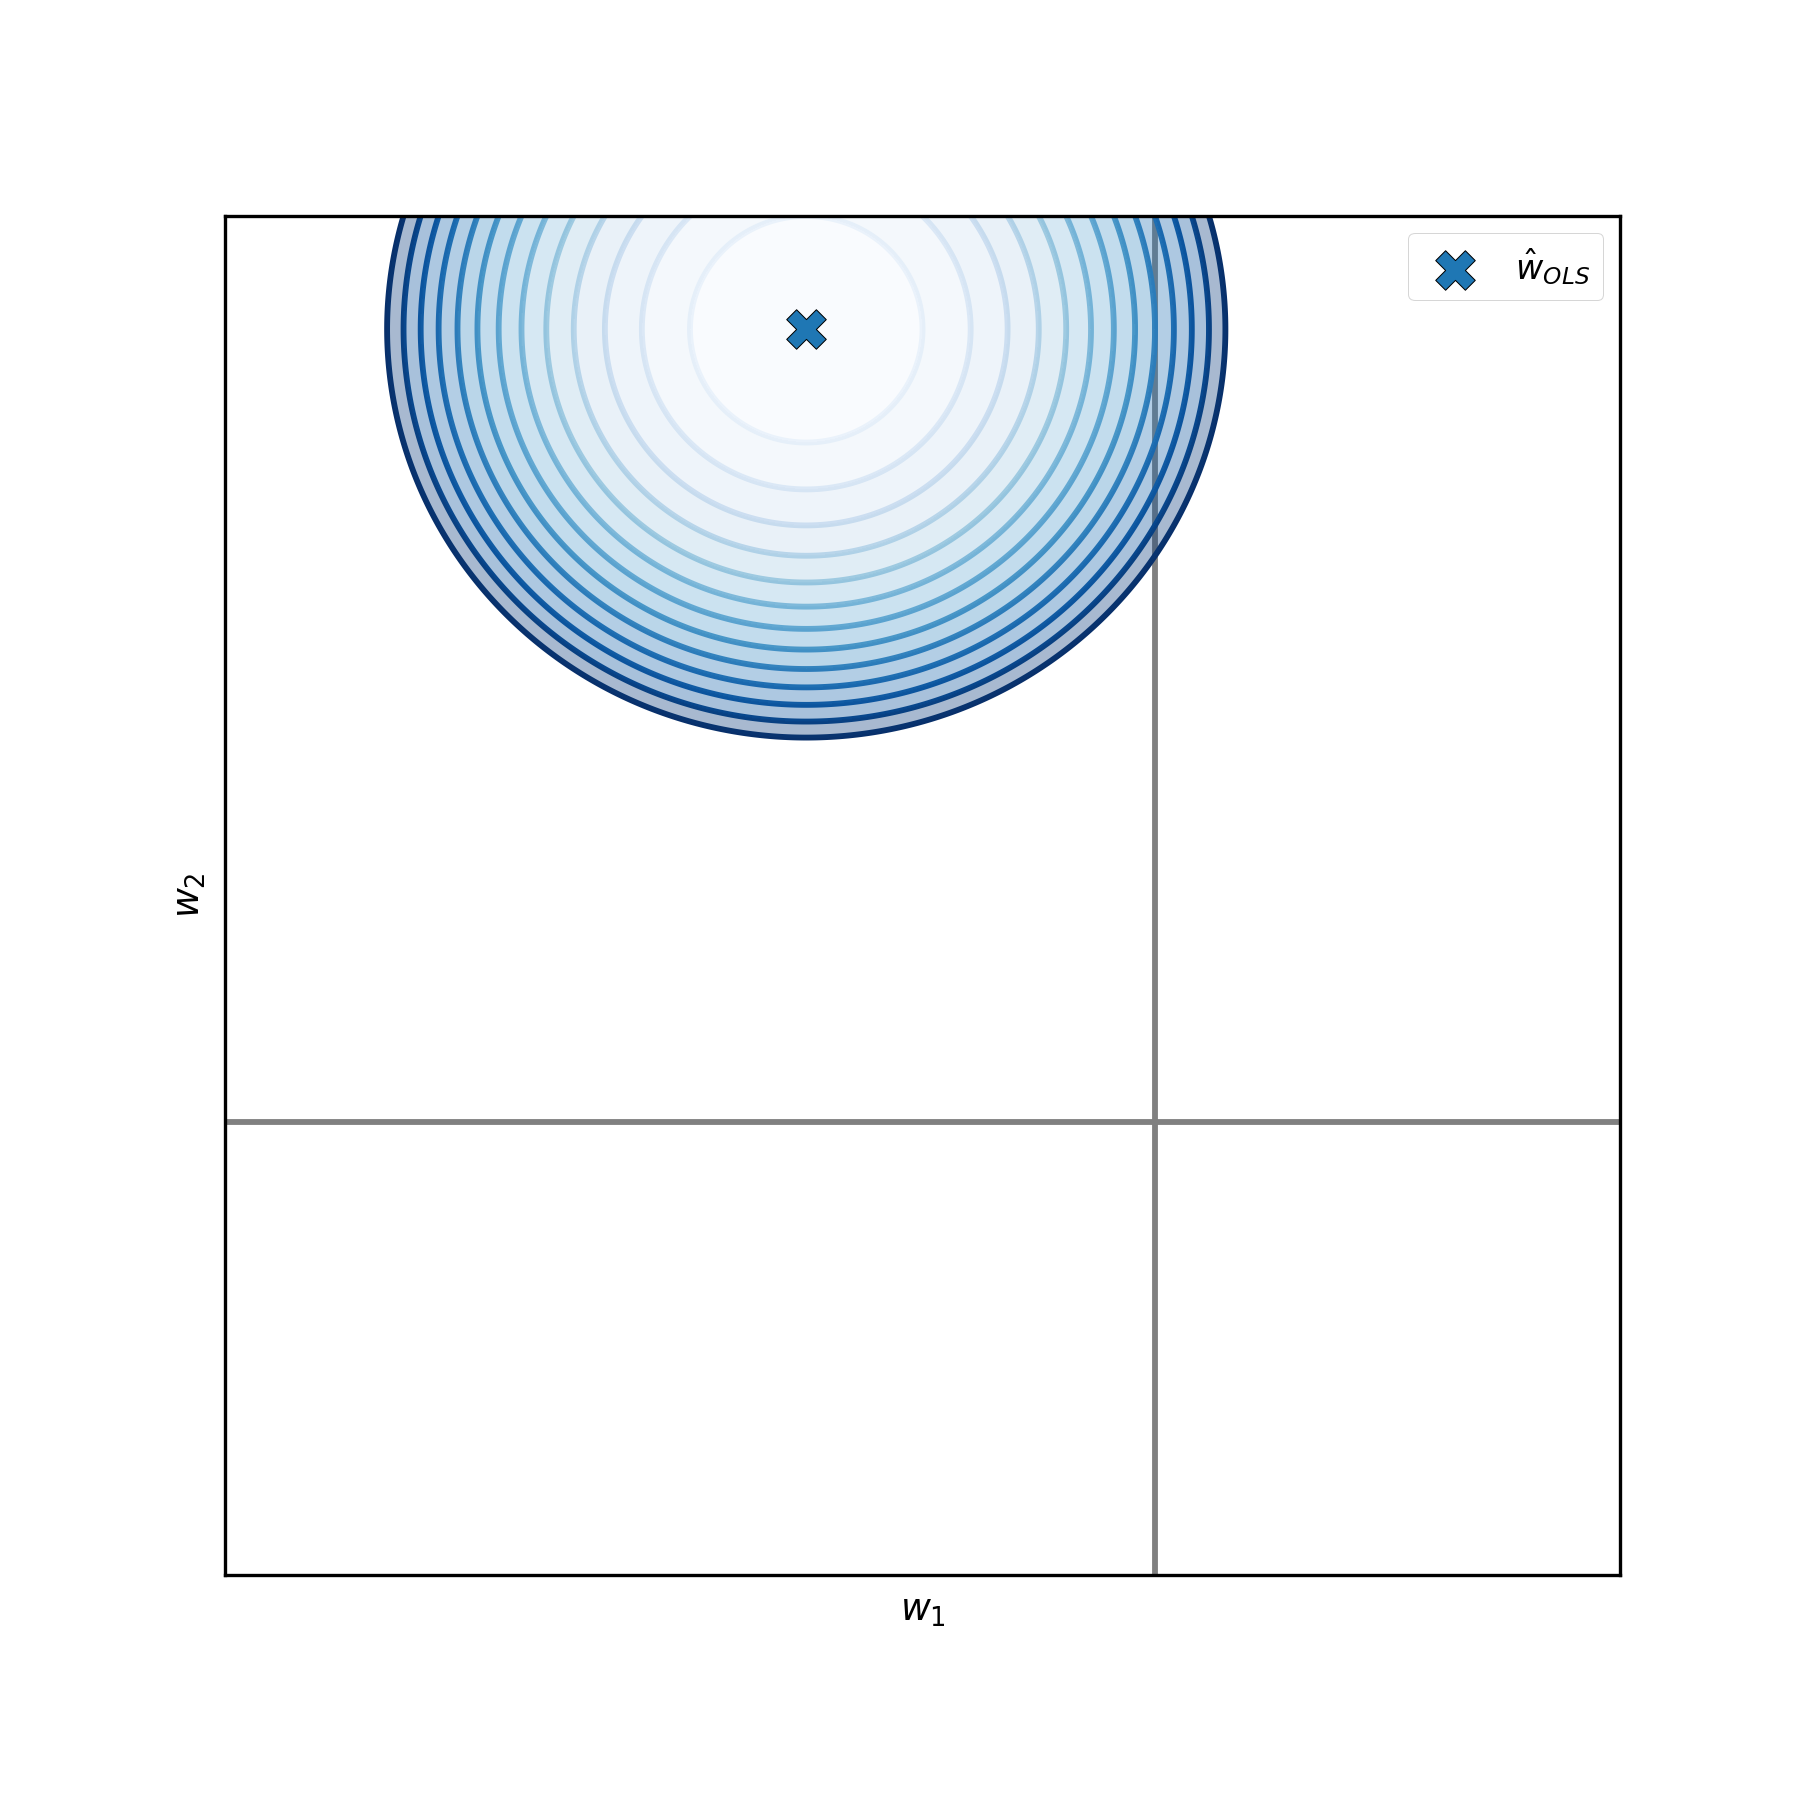
\includegraphics[width=0.5\textwidth]{part1/w_ols.png}
					\label{fig:w_ols}%
				}%
				%\hfill%
				\subfloat[]{%
					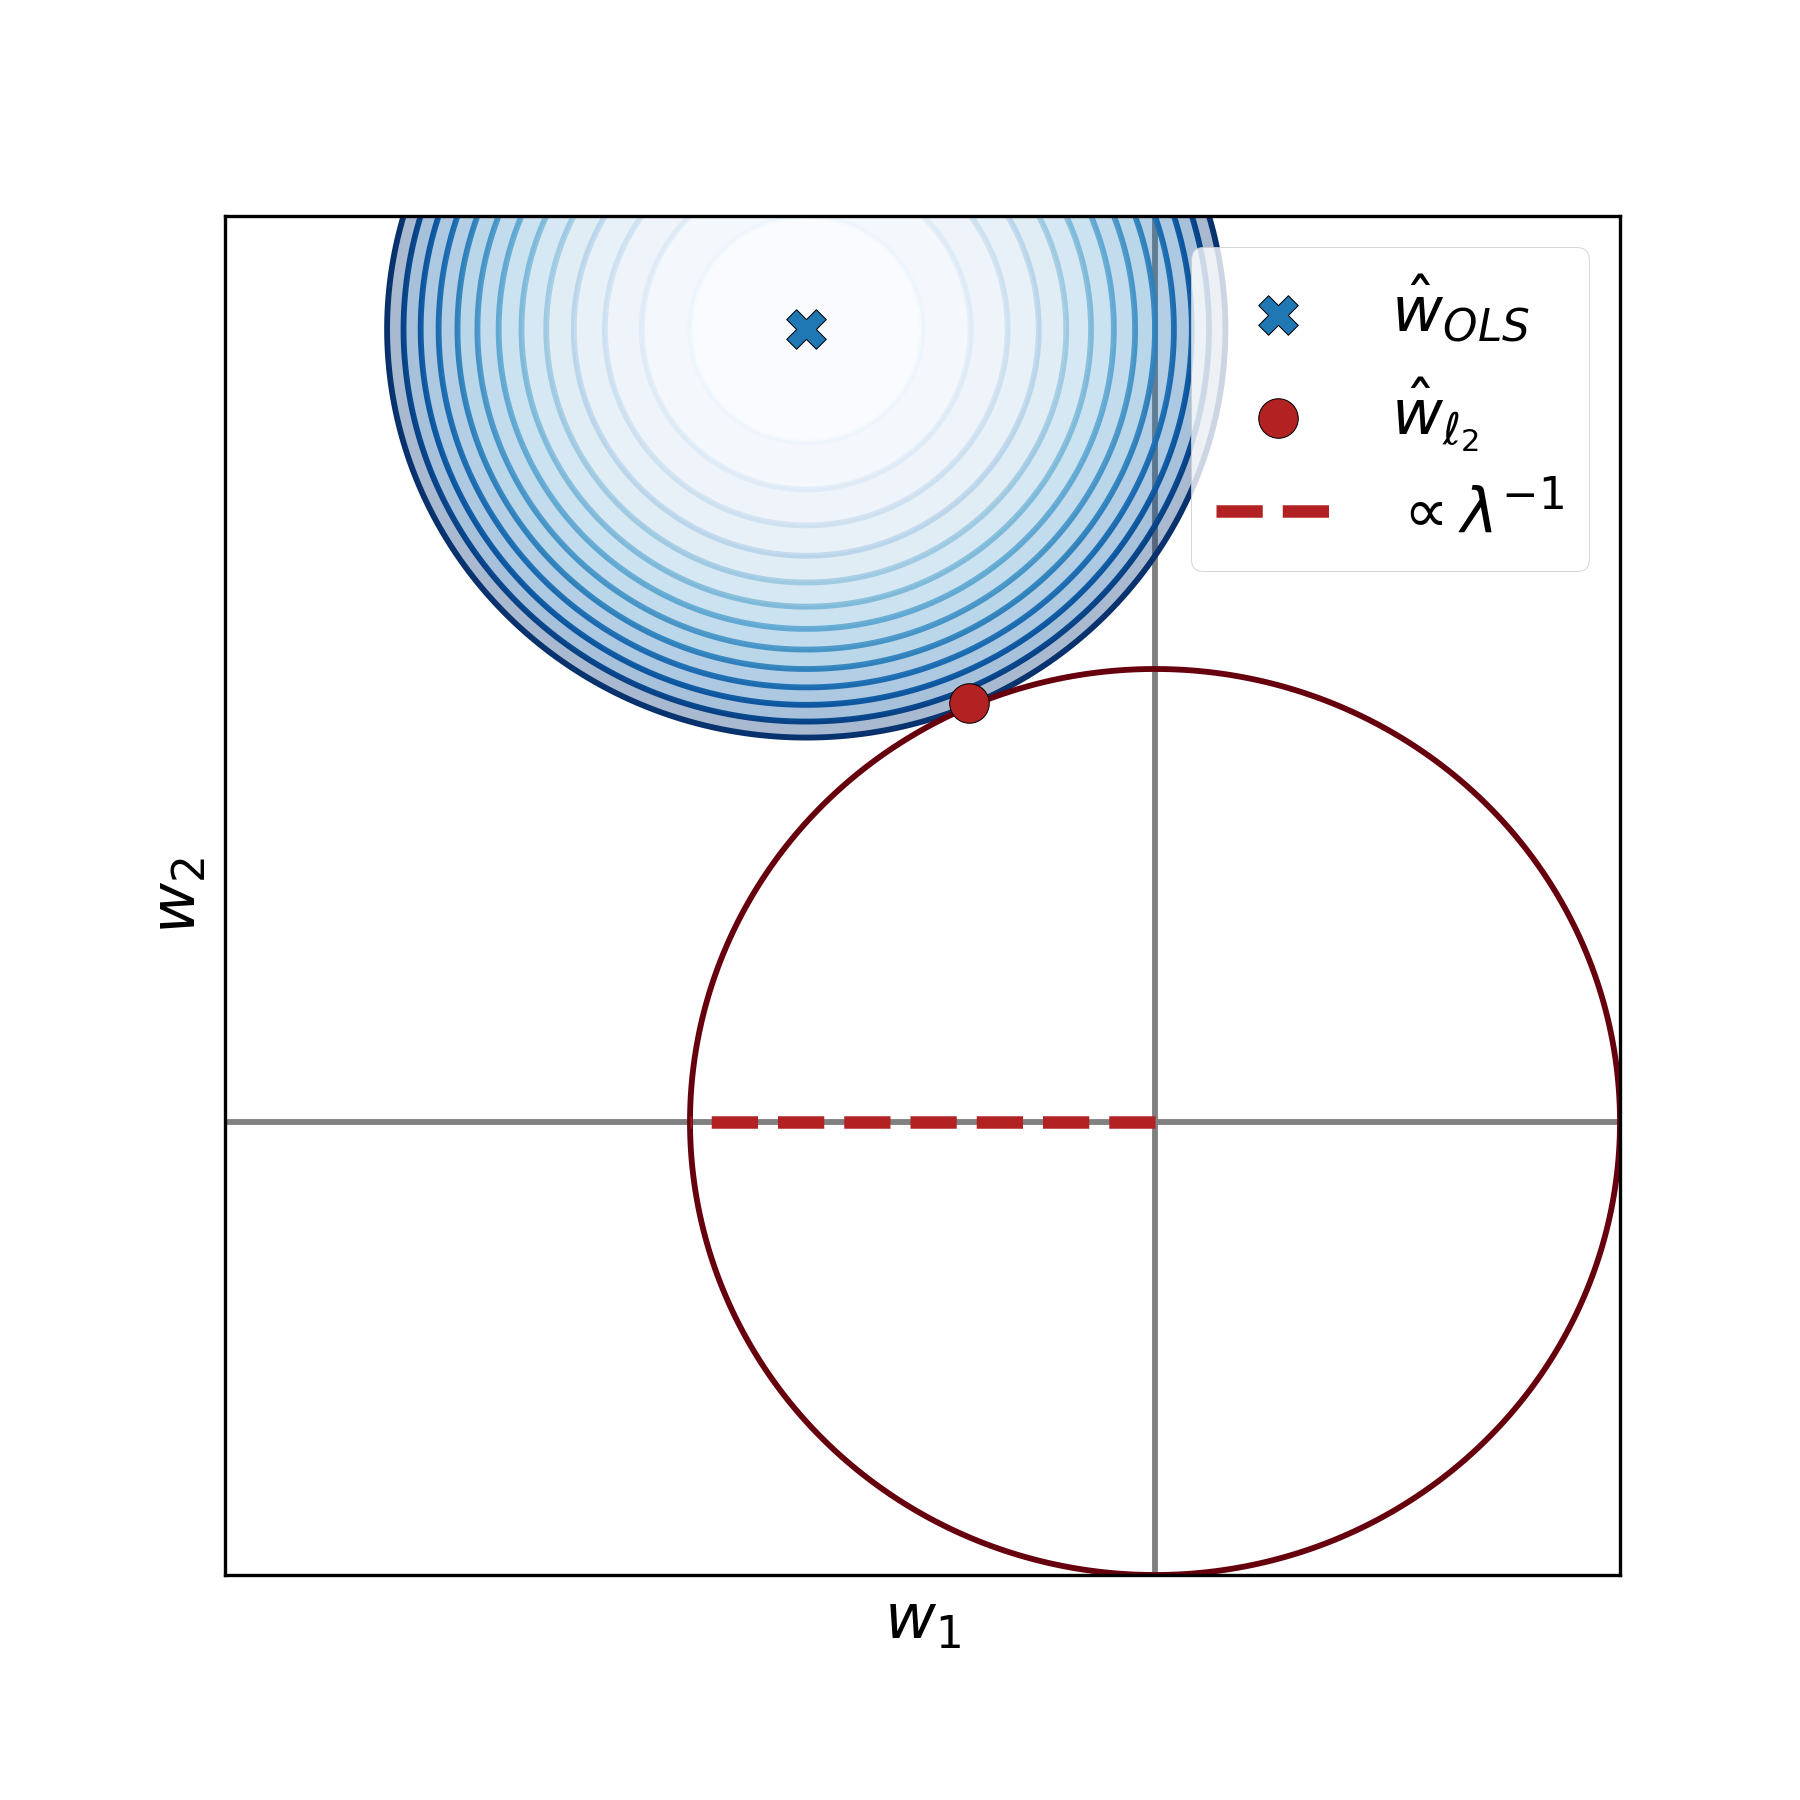
\includegraphics[width=0.5\textwidth]{part1/w_ridge.png}
					\label{fig:w_ridge}%
				}%
				\hfill%
				\subfloat[]{%
					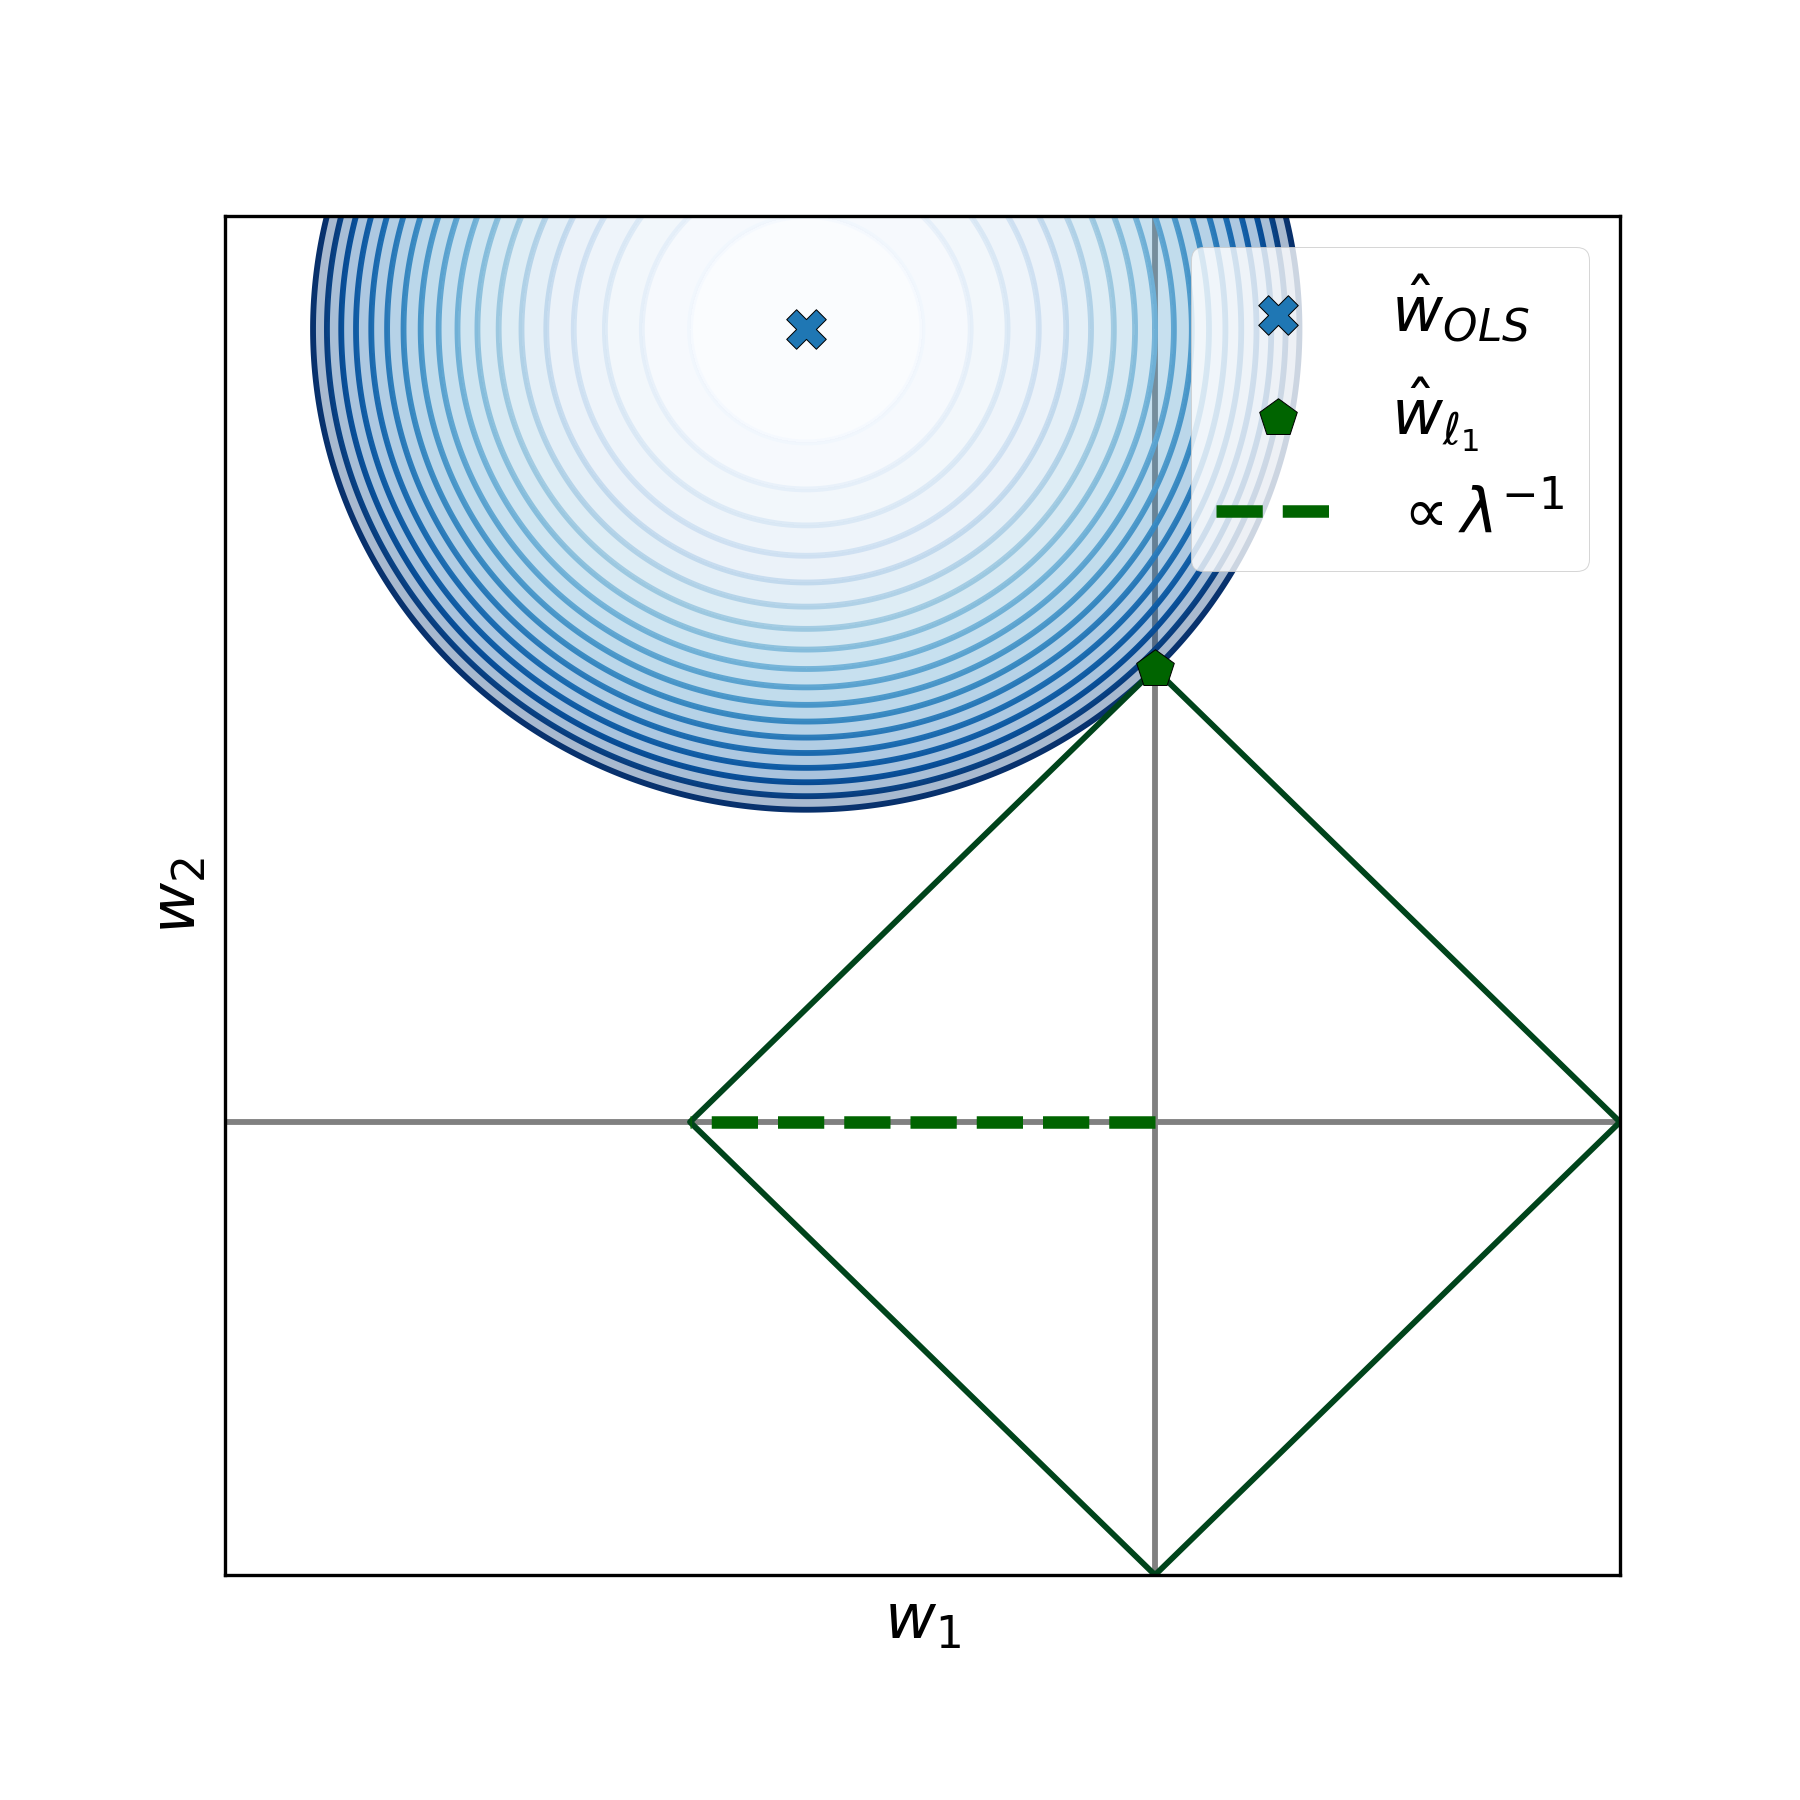
\includegraphics[width=0.5\textwidth]{part1/w_lasso.png}
					\label{fig:w_lasso}%
				}%
				%\hfill%
				\subfloat[]{%
					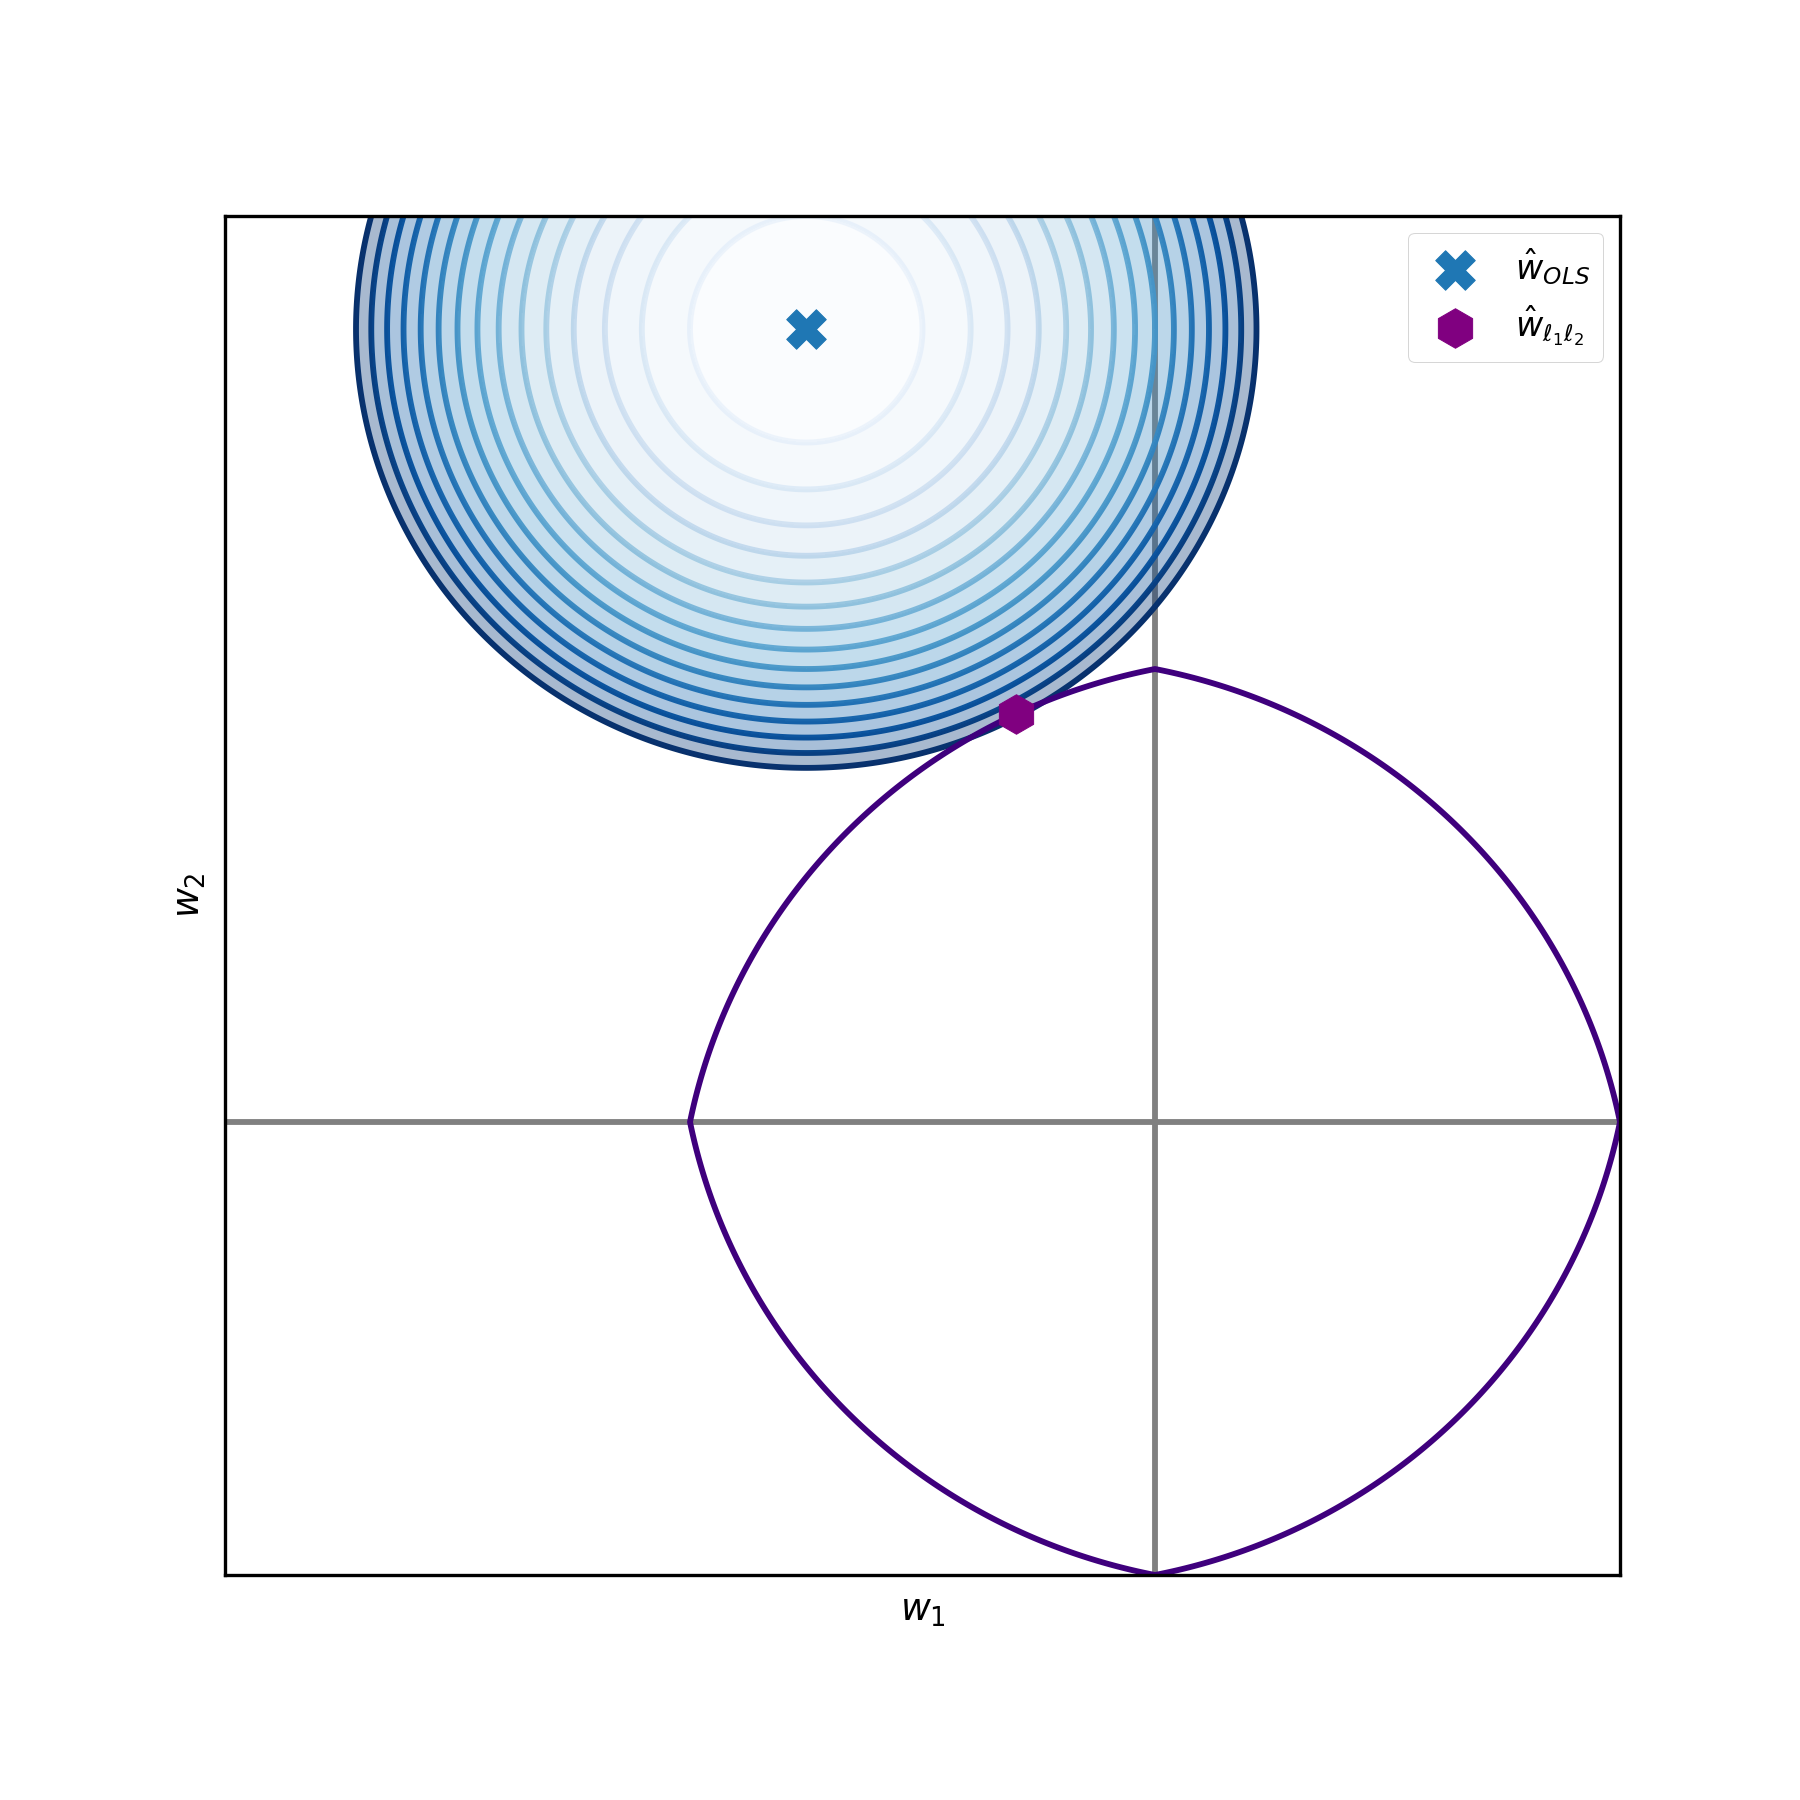
\includegraphics[width=0.5\textwidth]{part1/w_enet.png}
					\label{fig:w_enet}%
				}%
				\caption{Pictorial representation of the contour lines of the square loss in a 2D regression problem with various penalties: (a) ordinary least squares (no penalty), (b) ridge regression ($\ell_2$-norm penalty), (c) the Lasso ($\ell_1$-norm penalty) and finally (d) the Elastic-Net ($\ell_1$- and $\ell_2$-norm penalties).} \label{fig:square_loss_penalties}
			\end{figure}

			%%%%%%%%%%%%%%%%%%%%%%%%%%%%%%%%%%%%%%%
			% \subsubsection{Other sparsity-inducing penalties} \label{sec:other_sparsity}
			% asd

			% \begin{table}[htb]
			% 	\centering
			% 	\caption{Overview of the matrix norms used for vector-valued regression.}\label{tab:norms}
			% 	\begin{tabular}{l|l|l}
			% 		\toprule
			% 		Matrix norm  & Notation         & Definition                      \\  \midrule
			% 		Frobenius        & $\norm{A}_F$     & $\sqrt{\text{trace}(A^TA)}$     \\ [0.05cm]
			% 		Nuclear          & $\norm{A}_*$     & $\text{trace}\sqrt{(A^TA)}$     \\ [0.05cm]
			% 		Mixed $\text{L}_{2,1}$        & $\norm{A}_{2,1}$ & $\sum_{j}\norm{\bm{a}_j}_2$ \\ \bottomrule
			% 	\end{tabular}
			% \end{table}

			%%%%%%%%%%%%%%%%%%%%%%%%%%%%%%%%%%%%%%%
			\subsubsection{Logistic Regression} \label{sec:logistic_regression}
			Logistic regression is one of the most popular linear methods for classification problems\footnote{as counter-intuitive as it sounds}. In its unpenalized form, it can be simply seen as the problem of minimizing the logistic loss (see Table~\ref{tab:losses}) on a given training dataset. Therefore, logistic regression can be written as in Equation~\eqref{eq:logistic_regression},
			\begin{equation} \label{eq:logistic_regression}
				\bm{\hat w}_{\text{LR}} = \argmin_{\bm{w} \in \mathbb{R}^d} \frac{1}{n}\sum_{i=1}^n\log(1 + e^{-y_i\,\bm{x}_i^T\bm{w}})
			\end{equation}
			where the labels $y_i \in \{+1,-1\}, \forall i=1,\dots,n$. The minimization problem above is convex and differentiable, although as the gradient is nonlinear in $\bm{w}$, it does not have a closed-form solution. So, unpenalized logistic regression problems are typically solved by (stochastic) gradient descent-like techniques~\cite{boyd2004convex, sra2012optimization}.

			Unpenalized logistic regression, although theoretically sound, is somewhat uncommon in recent real-world studies. As already seen for the square loss, regularization penalties are typically used. For instance, we can have $\ell_2$-regularized logistic regression,
			\begin{equation} \label{eq:logistic_l2}
				\bm{\hat w}_{\ell_2} = \argmin_{\bm{w} \in \mathbb{R}^d} \frac{1}{n}\sum_{i=1}^n\log(1 + e^{-y_i\,\bm{x}_i^T\bm{w}}) + \lambda \norm{\bm{w}}_2^2
		  \end{equation}
			or various forms of sparse logistic regression such as
			\begin{equation} \label{eq:logistic_l1}
				\bm{\hat w}_{\ell_1} = \argmin_{\bm{w} \in \mathbb{R}^d} \frac{1}{n}\sum_{i=1}^n\log(1 + e^{-y_i\,\bm{x}_i^T\bm{w}}) + \lambda |\bm{w}|_1
		  \end{equation}
			which uses the Lasso penalty, or
			\begin{equation} \label{eq:logistic_l1l2}
				\bm{\hat w}_{\ell_1\ell_2} = \argmin_{\bm{w} \in \mathbb{R}^d} \frac{1}{n}\sum_{i=1}^n\log(1 + e^{-y_i\,\bm{x}_i^T\bm{w}}) + \lambda [\alpha |\bm{w}|_1 + (1-\alpha) \norm{\bm{w}}_2^2]
		  \end{equation}
			which uses the Elastic-Net penalty.
      The sparse logistic regression minimization problem can be efficiently solved either by proximal forward-backward splitting strategies (\eg FISTA~\cite{beck2009fast}), or by coordinate descent~\cite{wu2008coordinate}.

			Moreover, multi-class classification with logistic regression can be achieved by OVO, AVA approaches, as well as with the multiclass generalization of logistic regression: \textit{softmax} regression~\cite{hastie2009elements} (\aka multinomial logistic regression), which can be expressed as
			\begin{equation} \label{eq:softmax}
				\hat W_{\text{LR}} = \argmin_{W \in \mathbb{R}^{d \times k}} -\frac{1}{n} \bigg[ \sum_{i=1}^n \sum_{t=1}^k \mathds{1}\{y_i = t\} \log \bigg(\frac{e^{\bm{x}_i^T\bm{w}^t}}{\sum_{l=1}^k e^{\bm{x}_i^T \bm{w}^l}} \bigg) \bigg]
			\end{equation}
			where the indicator function $\mathds{1}\{\cdot\}$ includes in the functional only the correctly classified samples.

			%%%%%%%%%%%%%%%%%%%%%%%%%%%%%%%%%%%%%%%
			\subsubsection{Support Vector Machine}
			Support Vector Machine (\ac{SVM}) is a class of powerful algorithms that can be written as a penalized model and that can used for both regression (\ac{SVR}) and classification (\ac{SVC}) problems~\cite{evgeniou2000regularization}. In the first case, the adopted loss function is Vapnik's $\varepsilon$-insensitive loss:
			\begin{equation} \label{eq:epsilon_insensitive}
				|y - \bm{x}^T\bm{w}|_\varepsilon =
   			\begin{cases}
					0 & \text{if } |y-\bm{x}^T\bm{w}| < \varepsilon\\
					|y-\bm{x}^T\bm{w}| - \varepsilon & \text{otherwise}
				\end{cases}
			\end{equation}
			and in the second case the Hinge loss:
			\begin{equation} \label{eq:hinge_loss}
				|1 - y\,\bm{x}^T\bm{w}|_+ = \max[0, 1 - y\,\bm{x}^T\bm{w}]
			\end{equation}
			as reported in Table~\ref{tab:losses} and shown in Figures~\ref{fig:regression}~\ref{fig:classification}. The standard formulation of SVM is penalized with the $\ell_2$-norm~\cite{vapnik2013nature}.
			Therefore, sticking to linear models, the SVR minimization problem can be written as
			\begin{equation} \label{eq:svr}
				\bm{\hat w}_{\text{SVR}} = \argmin_{\bm{w} \in \mathbb{R}^d} \frac{1}{n} \sum_{i=1}^n |y_i - f(\bm{x}_i)|_\varepsilon + \lambda \norm{\bm{w}}_2^2
			\end{equation}
			while the SVC minimization problem is
			\begin{equation} \label{eq:svc}
				\bm{\hat w}_{\text{SVC}} = \argmin_{\bm{w} \in \mathbb{R}^d} \frac{1}{n} \sum_{i=1}^n |1 - y_if(\bm{x}_i)|_+ + \lambda \norm{\bm{w}}_2^2
			\end{equation}
			where, as usually, $\lambda$ controls the trade-off between data adherence and smoothing of the solution.
			Equations~\eqref{eq:svr} and~\eqref{eq:svc} are known as the \textit{primal} SVM problem. However, in order to generalize the SVM to nonlinear cases (see Section~\ref{sec:kernel_trick}), it is often convenient to transform this minimization problem in its \textit{dual} form. Several algorithms to find the solution of the SVM minimization problem in both primal and dual forms were developed, such as Newton's method or coordinate descent algorithm, see~\cite{smola2004tutorial, shawe2011review} for an exhaustive review.

			The standard formulation of SVM does not cope well with high-dimensional data, as no sparsity-enforcing penalty is adopted. Recently, $\ell_1$-norm penalized SVM were proposed as well in~\cite{zhu20041, peng2016error}.

			As for the square loss-based methods, let's apply ($\ell_2$-penalized) SVR to the aging problem (introduced in Section~\ref{sec:ols}).
			The experimental setup in this case is the same already adopted for Lasso and ridge regression (see Sections~\ref{sec:the_lasso}~\ref{sec:ridge_regression}).
			The weights $\bm{\hat w}_{\text{SVR}}$ are represented in Figure~\ref{fig:coefs_svr}. As expected, none of the is exactly zero and they look similar to ridge coefficients in Figure~\ref{fig:coefs_ridge}, as the two model share the same regularization penalty.
			\begin{figure}[!h]
				\centering
				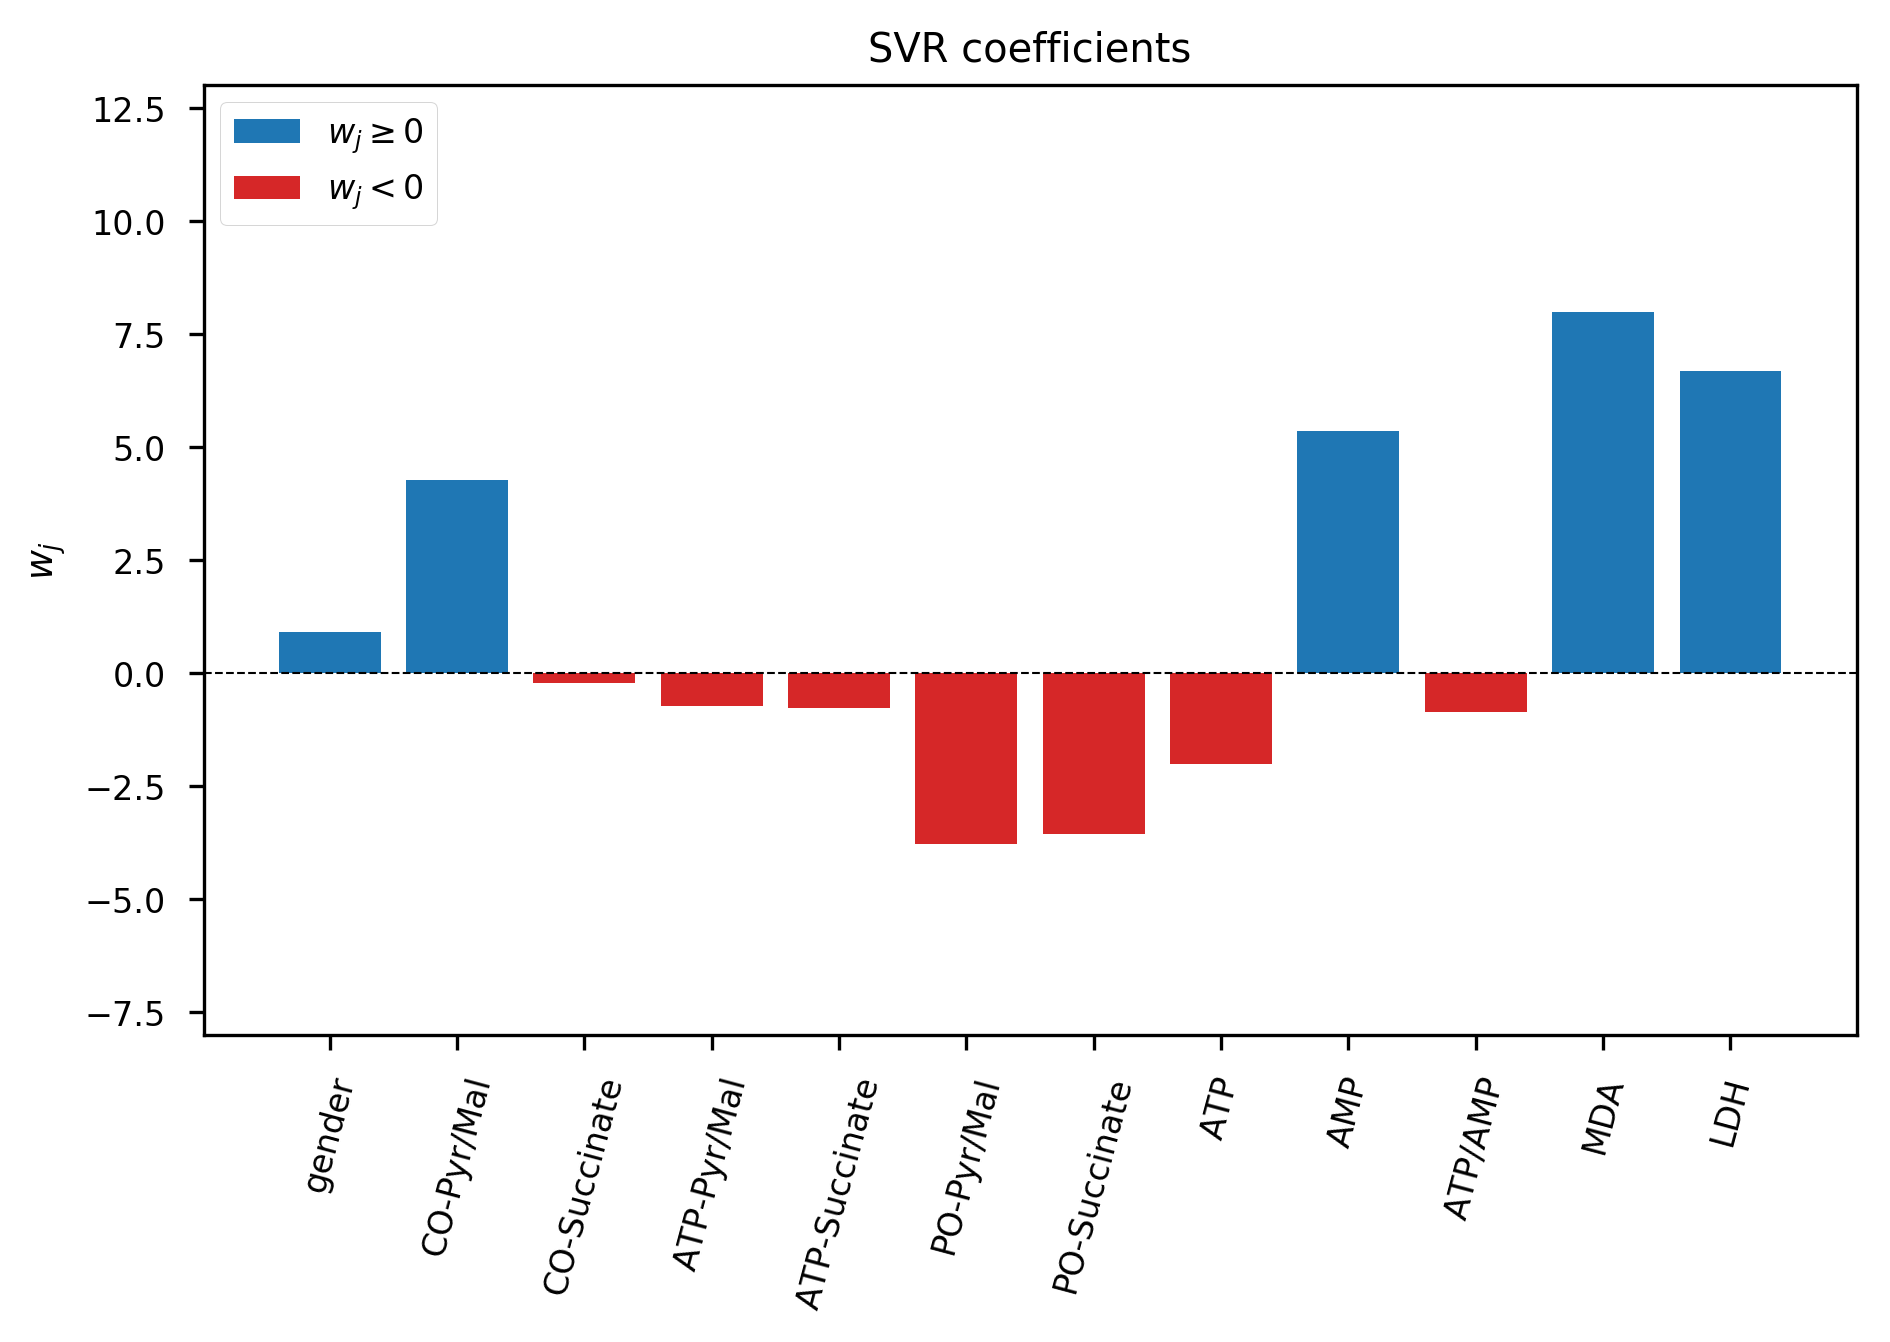
\includegraphics[width=0.8\textwidth]{part1/coefs_svr.png}
				\caption{A pictorial representation of the vector $\bm{\hat w}_{\text{SVR}}$ obtained fitting a SVR model on $74$ randomly selected training samples of $\mathcal{D}_{\text{aging}}$. Variables associated with positive (\ie directly proportional to the output) and a negative (\ie inversely proportional) weight are represented in blue and red, respectively.} \label{fig:coefs_svr}
			\end{figure}
			Evaluating $\bm{\hat w}_{\text{SVR}}$ on the test set, the SVR model has $\text{MAE}=9.280$ and explains the $77.74\%$ of the variance.

			% \begin{enumerate}
			% 	\item loss: hinge
			% 	\item dual problem?
			% 	\item penalties: l2 + l1
			% 	\item use in classification and regression
			% 	\item extension to multiple-class? (not sure)
			% 	\item use cases
			% \end{enumerate}

			%%%%%%%%%%%%%%%%%%%%%%%%%%%%%%%%%%%%%%%%%%%%%%%%%%%%%%%%%%%%%%%%%%%
			\subsection{The kernel trick} \label{sec:kernel_trick}
			For ease of reading, all the regularization methods presented so far were focused on learning linear input-output relationships $y = \bm{x}^T\bm{w}$. Actually, they can all be extended to the nonlinear case exploiting the so-called \textit{kernel trick}.

			The basic idea of the kernel trick is to use a map that projects the features on a higher (possibly infinite) dimensional space in which the prediction problem is, to some extent, easier to solve. An example of kernel trick for nonlinear classification problem is presented in Figure~\ref{fig:kernel_trick}.

			\begin{figure}[!h]
				\centering
				\subfloat[]{%
					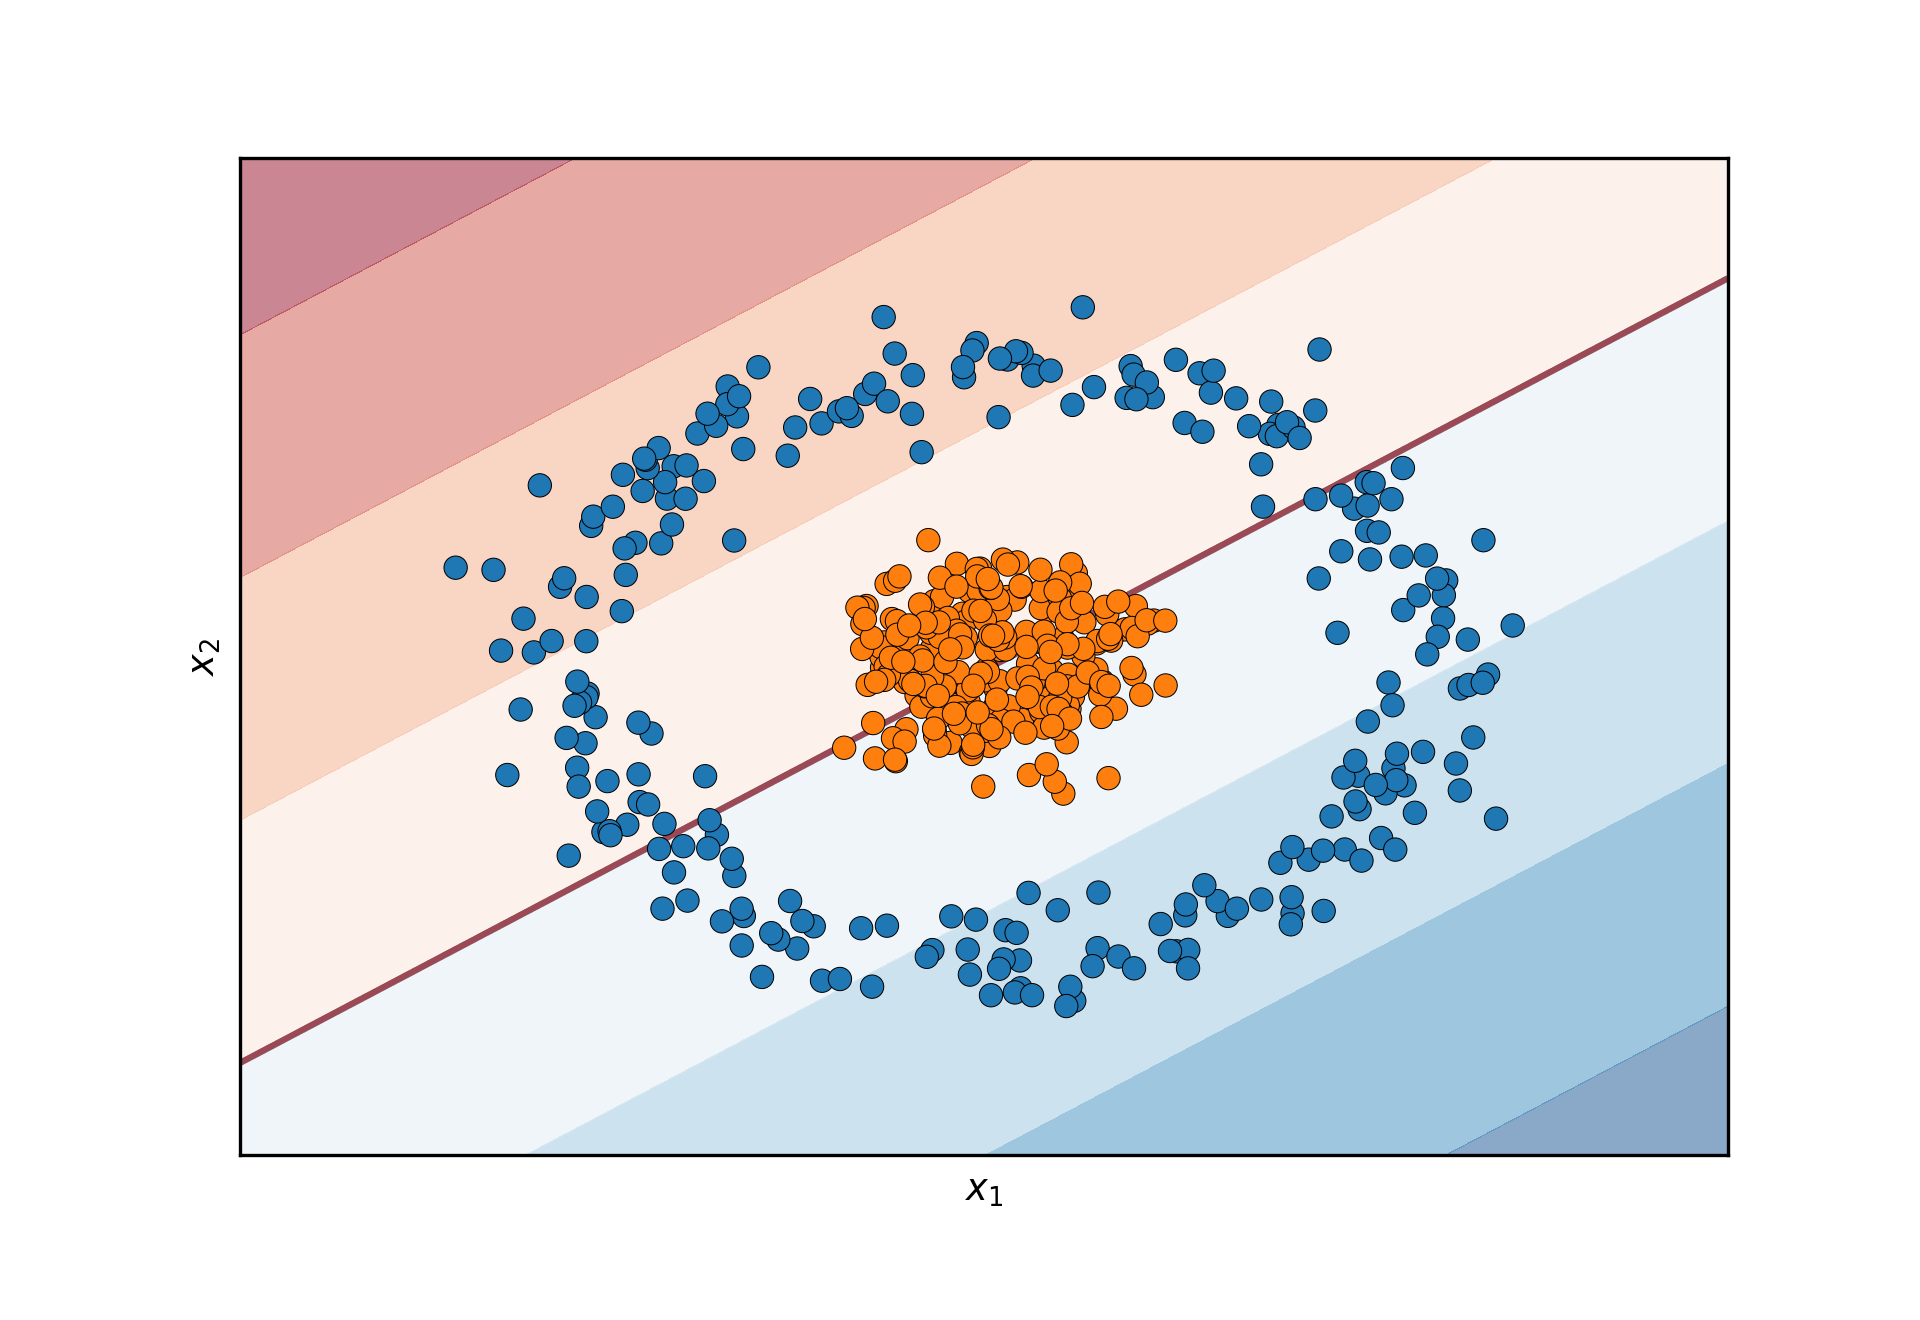
\includegraphics[width=0.5\textwidth]{part1/kernel_trick0.png}
					\label{fig:kernel_trick0}%
				}%
				%\hfill%
				\subfloat[]{%
					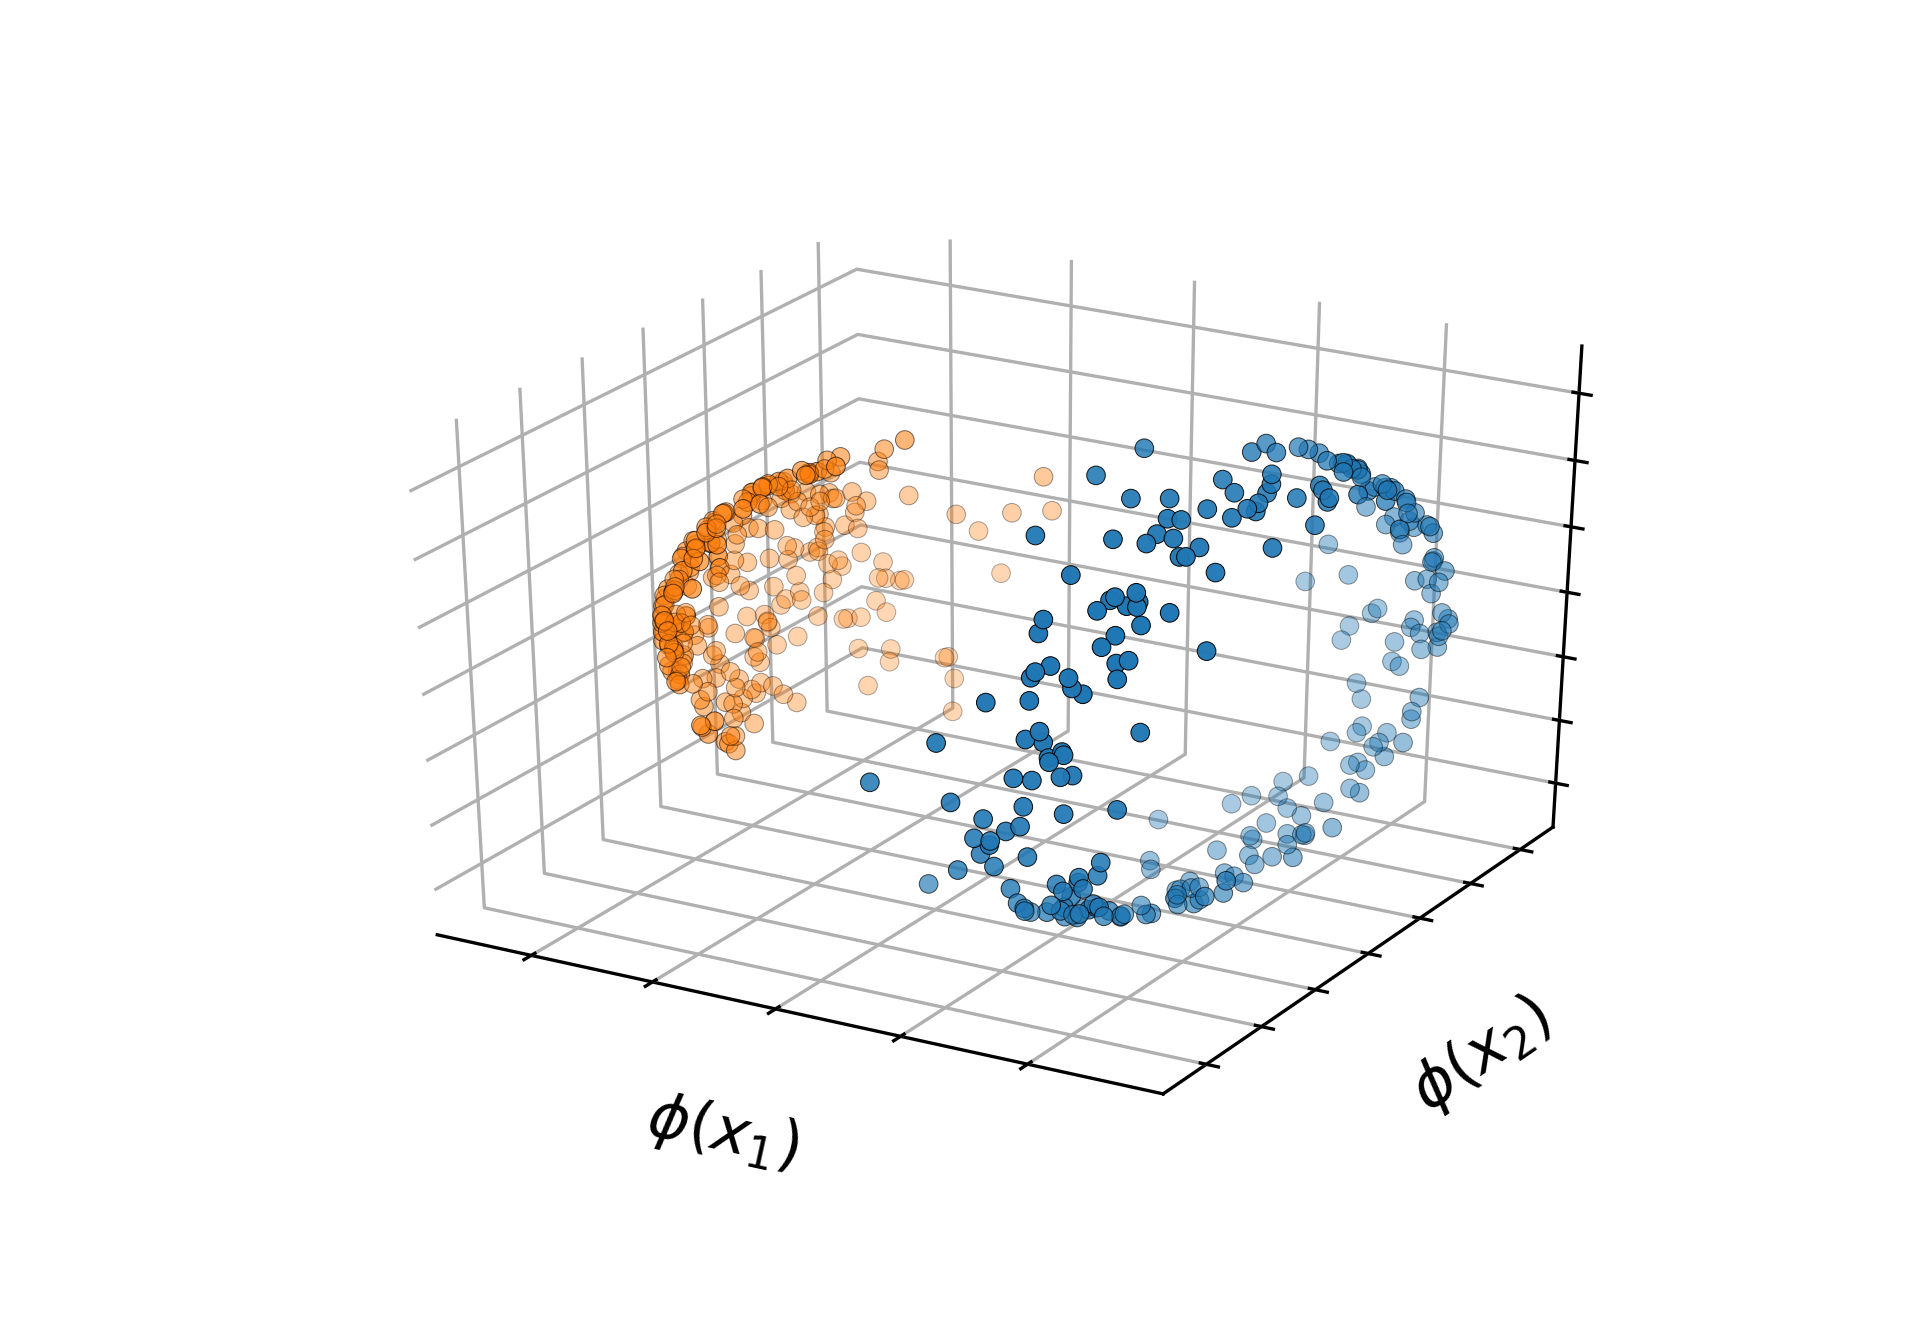
\includegraphics[width=0.5\textwidth]{part1/kernel_trick1.png}
					\label{fig:kernel_trick1}%
				}%
				\hfill%
				\subfloat[]{%
					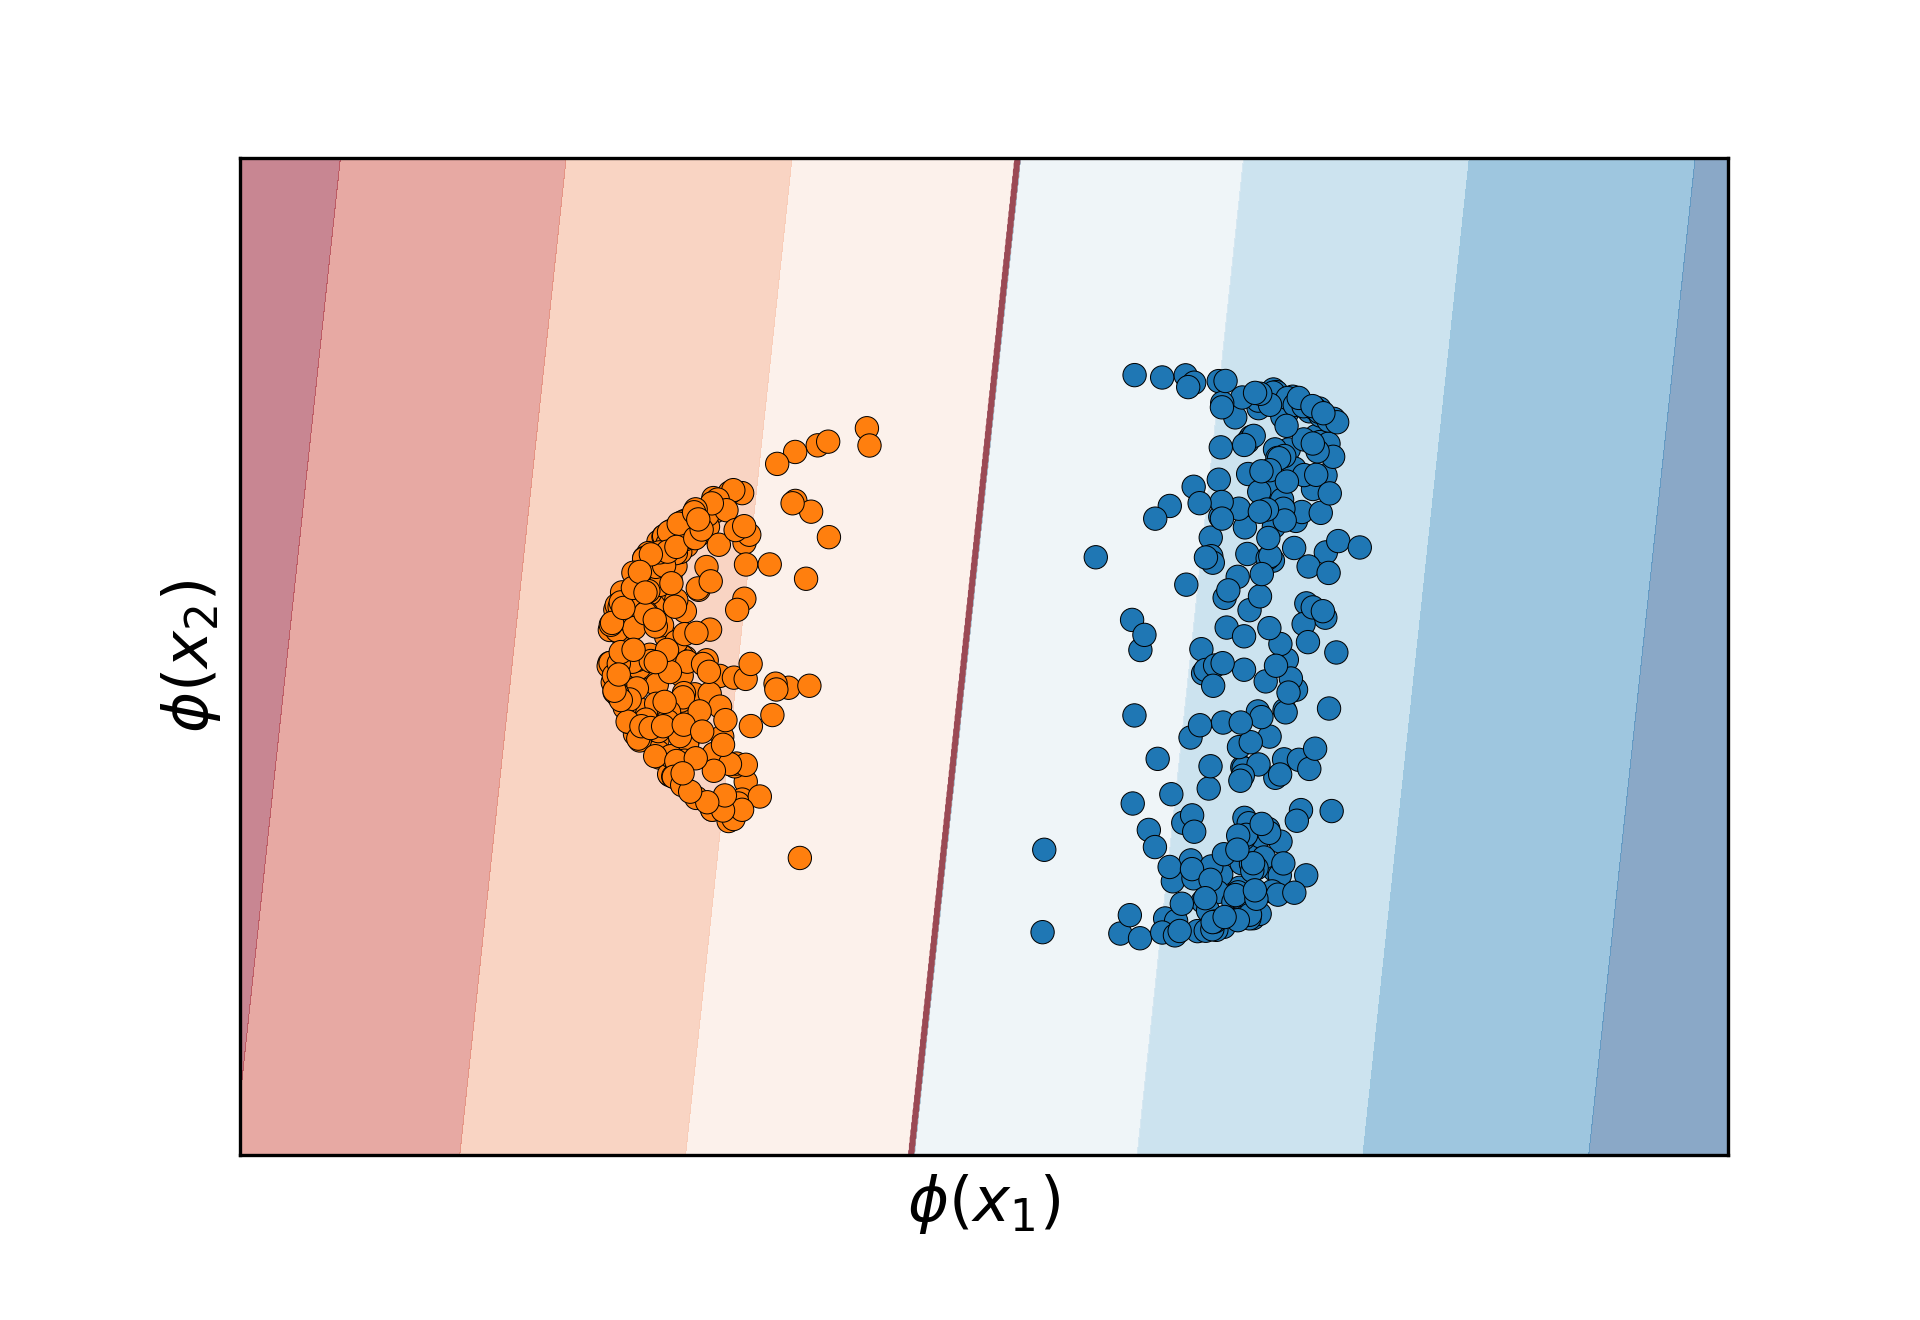
\includegraphics[width=0.5\textwidth]{part1/kernel_trick2.png}
					\label{fig:kernel_trick2}%
				}%
				\caption{Pictorial representation of the kernel trick. Panel (a) shows a 2D classification problem where the input-output relationship is nonlinear. Panel (b) shows the \textit{kernel explosion}, \ie the projection of the 2D problem in a higher (3D) dimensional space in which the two classes are linearly separable, as shown in Panel (c).}\label{fig:kernel_trick}
			\end{figure}

			We define the nonlinear feature mapping function as $\phi: \mathcal{X} \rightarrow \mathcal{F}$; for instance $\mathcal{X} \in \mathbb{R}^d$ and $\mathcal{F} \in \mathbb{R}^p$ with $p \geq d$, or even $p \gg d$.
			Given $\phi$, the representer theorem~\cite{smola1998learning}, states that the learning problem of Equation~\eqref{eq:losspen} admits a solution of the form
			$$
			\hat f(\bm{x}) = \sum_{i=1}^n k(\bm{x}_i, \bm{x}_j) \alpha_i
			$$
			where $\bm{\alpha} \in \mathbb{R}^n$ and the function $k$ behaves like an inner product, \ie it is: symmetric, positive definite, ad it can be defined as in Equation~\eqref{eq:kernel_function}.
			\begin{equation} \label{eq:kernel_function}
				k(\bm{x}_i, \bm{x}_j) =  \phi{(\bm{x}_i)}^T \cdot \phi{(\bm{x}_j)} % = \langle \phi{(\bm{x}_i)}, \phi{(\bm{x}_j)} \rangle_{\mathcal{H}}
			\end{equation}
			In the ML literature, $k$ is typically called the \textit{kernel} function and it comes in handy to solve the dual version of the learning problems.

			% Following~\cite{evgeniou2000regularization}, we assume that $\mathcal{F}$ is a Reproducing Kernel Hilbert Space (RKHS) $\mathcal{H}$.
			% Given $\phi$, the nonlinear input-output relationship can be formulated as
			% $$
			% f(\bm{x}) = \phi(\bm{x})^T\bm{w}
			% $$
			% which, nevertheless, is linear in its parameters $\bm{w}$.
      %
			% In this context it is easy to see that every feature map defines the positive definite function $k$ of Equation~\eqref{eq:kernel_function}.
			% \begin{equation} \label{eq:kernel_function}
			% 	k(\bm{x}_i, \bm{x}_j) =  \phi{(\bm{x}_i)}^T \cdot \phi{(\bm{x}_j)} % = \langle \phi{(\bm{x}_i)}, \phi{(\bm{x}_j)} \rangle_{\mathcal{H}}
			% \end{equation}
			% Therefore, for fixed loss function and regularization penalty, a kernel machine can be written as
			% \begin{equation} \label{eq:kernel_learning_problem}
			% 	\hat f = \argmin_{f \in \mathcal{H}} \frac{1}{n} \sum_{i=1}^n L(f(\bm{x}_i), y_i) + \lambda \norm{f}^2_\mathcal{H}
			% \end{equation}
			% where $\norm{\cdot}_\mathcal{H}^2$ is the norm associated by the RKHS.
			% The problem in Equation~\eqref{eq:kernel_learning_problem}, for the
			% can be casted in the so-called \textit{dual} representation in which the outputs are predicted exploiting a \textit{kernel function} defined as in Equation~\eqref{eq:kernel_function}.

			Let's see a practical example: the kernel ridge regression. We recall that standard ridge regression problem can be rewritten as
			$$
			\bm{\hat w}_{\ell_2} = \argmin_{\bm{w} \in \mathbb{R}^d} J(\bm{w})
			$$
			where the objective function $J(\bm{w})$ is
			$$
			J(\bm{w}) = \frac{1}{n}\norm{X\bm{w}-\bm{w}}_2^2+\lambda\norm{\bm{w}}_2^2 = \frac{1}{n}(X\bm{w}-\bm{y})^T(X\bm{w}-\bm{y})+\lambda\bm{w}^T\bm{w}
			$$
			Therefore, the solution of the ridge regression problem can be evaluated by imposing $\frac{\partial J(\bm{w})}{\partial \bm{w}}=0$ which leads to the following linear system of equations.
			$$
			X^TX\bm{w}-X^T\bm{y}+\lambda n \bm{w}=0 \Rightarrow (X^TX+\lambda n I)\bm{w} = X^T\bm{y}
			$$
			This can either be solved with respect to $\bm{w}$ (see Section~\ref{sec:ridge_regression}) obtaining the solution of the \textit{primal} form
			\begin{equation} \label{eq:ridge_backup}
				\bm{w} = (X^TX+\lambda n I)^{-1}X^T\bm{y}
		  \end{equation}
			or it can be rewritten as
			$$
			\bm{w} = \frac{1}{\lambda n} X^T(\bm{y}-X\bm{w}) = X^T\bm{\alpha}
			$$
			where $\bm{\alpha} = \frac{1}{\lambda n}(\bm{y} - X\bm{w})$ is the \textit{dual} variable. Therefore, the dual formulation of the problem becomes
			$$
				\begin{aligned}
					\bm{\alpha} = {} & \frac{1}{\lambda n}(\bm{y} - X\bm{w}) \\
						{} & \Rightarrow \lambda n \bm{\alpha} = (\bm{y} - X\bm{w})\\
						{} & \Rightarrow \lambda n \bm{\alpha} = (\bm{y} - XX^T\bm{\alpha})\\
						{} & \Rightarrow (XX^T + \lambda n I) \bm{\alpha} = \bm{y}\\
				\end{aligned}
			$$
			\begin{equation} \label{eq:ridge_dual}
				\Rightarrow \bm{\alpha} = (K + \lambda n I)^{-1}\bm{y} \\
			\end{equation}
			where $K$ is the $n \times n$, symmetric and positive semi-definite kernel matrix, with entries $K_i^j = k(\bm{x}_i, \bm{x}_j)$. In this case $k(\bm{x}_i, \bm{x}_j) = \bm{x}_i^T\bm{x}_j$, and this corresponds to the linear kernel. Nevertheless, several other options are available (see Table~\ref{tab:kernels} or~\cite{bishop2006pattern} for more details). Choosing a different kernel for ridge regression simply boils down to choose a different formulation for the kernel function $k$, hence plugging the obtained kernel matrix $K$ in Equation~\eqref{eq:ridge_dual} to achieve the desired solution.

			The advantage of the kernel trick is not only statistical, but also computational. Indeed, we may notice that solving the primal problem (\ie in $\bm{w}$) requires $O(n^3)$ operations, while solving the dual (\ie in $\bm{\alpha}$) requires $O(d^3)$ operations which is better for large scale and relatively low-dimensional problem.

    	 \begin{table}[htb]
				\centering
				\caption{Popular kernel functions. \ac{RBF} stands for Radial Basis Function.}
				\label{tab:kernels}
				\begin{tabular}{@{}ll@{}}
					\toprule
					name       & formulation                                            \\ \midrule
					linear     & $k(\bm{x}, \bm{x}') =\bm{x}^T\bm{x}' $                               \\
					polynomial & $k(\bm{x},\bm{x}') = (\bm{x}^T\bm{x}' + c)^d$    \\
					RBF        & $k(\bm{x},\bm{x}') = e^{-\gamma\norm{\bm{x} - \bm{x}'}^2}$ \\
					sigmoid    & $k(\bm{x},\bm{x}') = \tanh(\gamma \bm{x}^T\bm{x}' + c)$ \\ \bottomrule
				\end{tabular}
			\end{table}

			A similar derivation can also be obtained applying the kernel trick to logistic regression and SVM~\cite{bishop2006pattern, shawe2004kernel}.
			
    	\begin{table}[htb]
			\centering
			\caption{Overview of the matrix norms used for multiple-output regression.}\label{tab:norms}
			\begin{tabular}{l|l|l}
				\toprule
				Matrix norm  & Notation         & Definition                      \\  \midrule
				Frobenius        & $\norm{A}_F$     & $\sqrt{\text{trace}(A^TA)}$     \\ [0.05cm]
				Nuclear          & $\norm{A}_*$     & $\text{trace}\sqrt{(A^TA)}$     \\ [0.05cm]
				Mixed $\text{L}_{2,1}$        & $\norm{A}_{2,1}$ & $\sum_{j}\norm{\bm{a}_j}_2$ \\ \bottomrule
			\end{tabular}
		\end{table}	

		%%%%%%%%%%%%%%%%%%%%%%%%%%%%%%%%%%%%%%%%%%%%%%%%%%%
		\subsection{Decision trees} \label{sec:decision_trees} 
		Decision trees are simple, yet powerful, methods for regression and classification.
		They are based on recursive binary splits of the feature space, in which they fit a very simple model, such as a constant.
		Fitting a decision tree on a given dataset results in partitioning the feature space in \textit{cuboid} regions with edges aligned to the axes.
		In each region, there is a separate model to predict the target variable. In regression problems this can be the average of the samples falling in the region, whereas for classification problems, it can be the assignment to the most represented class.
		In particular, when decision trees are applied to classification problems, the feature space partitioning aims at keeping samples with the same labels grouped together.
		In this thesis, we refer to one of the most popular method for decision tree-based classification and regression, known as \ac{CART}~\cite{breiman1984classification}.
		
		An example of application of this technique for classification and regression is shown in Figure~\ref{fig:decision_trees}.
		
		\begin{figure}[!ht]
			\centering
			\subfloat[]{%
				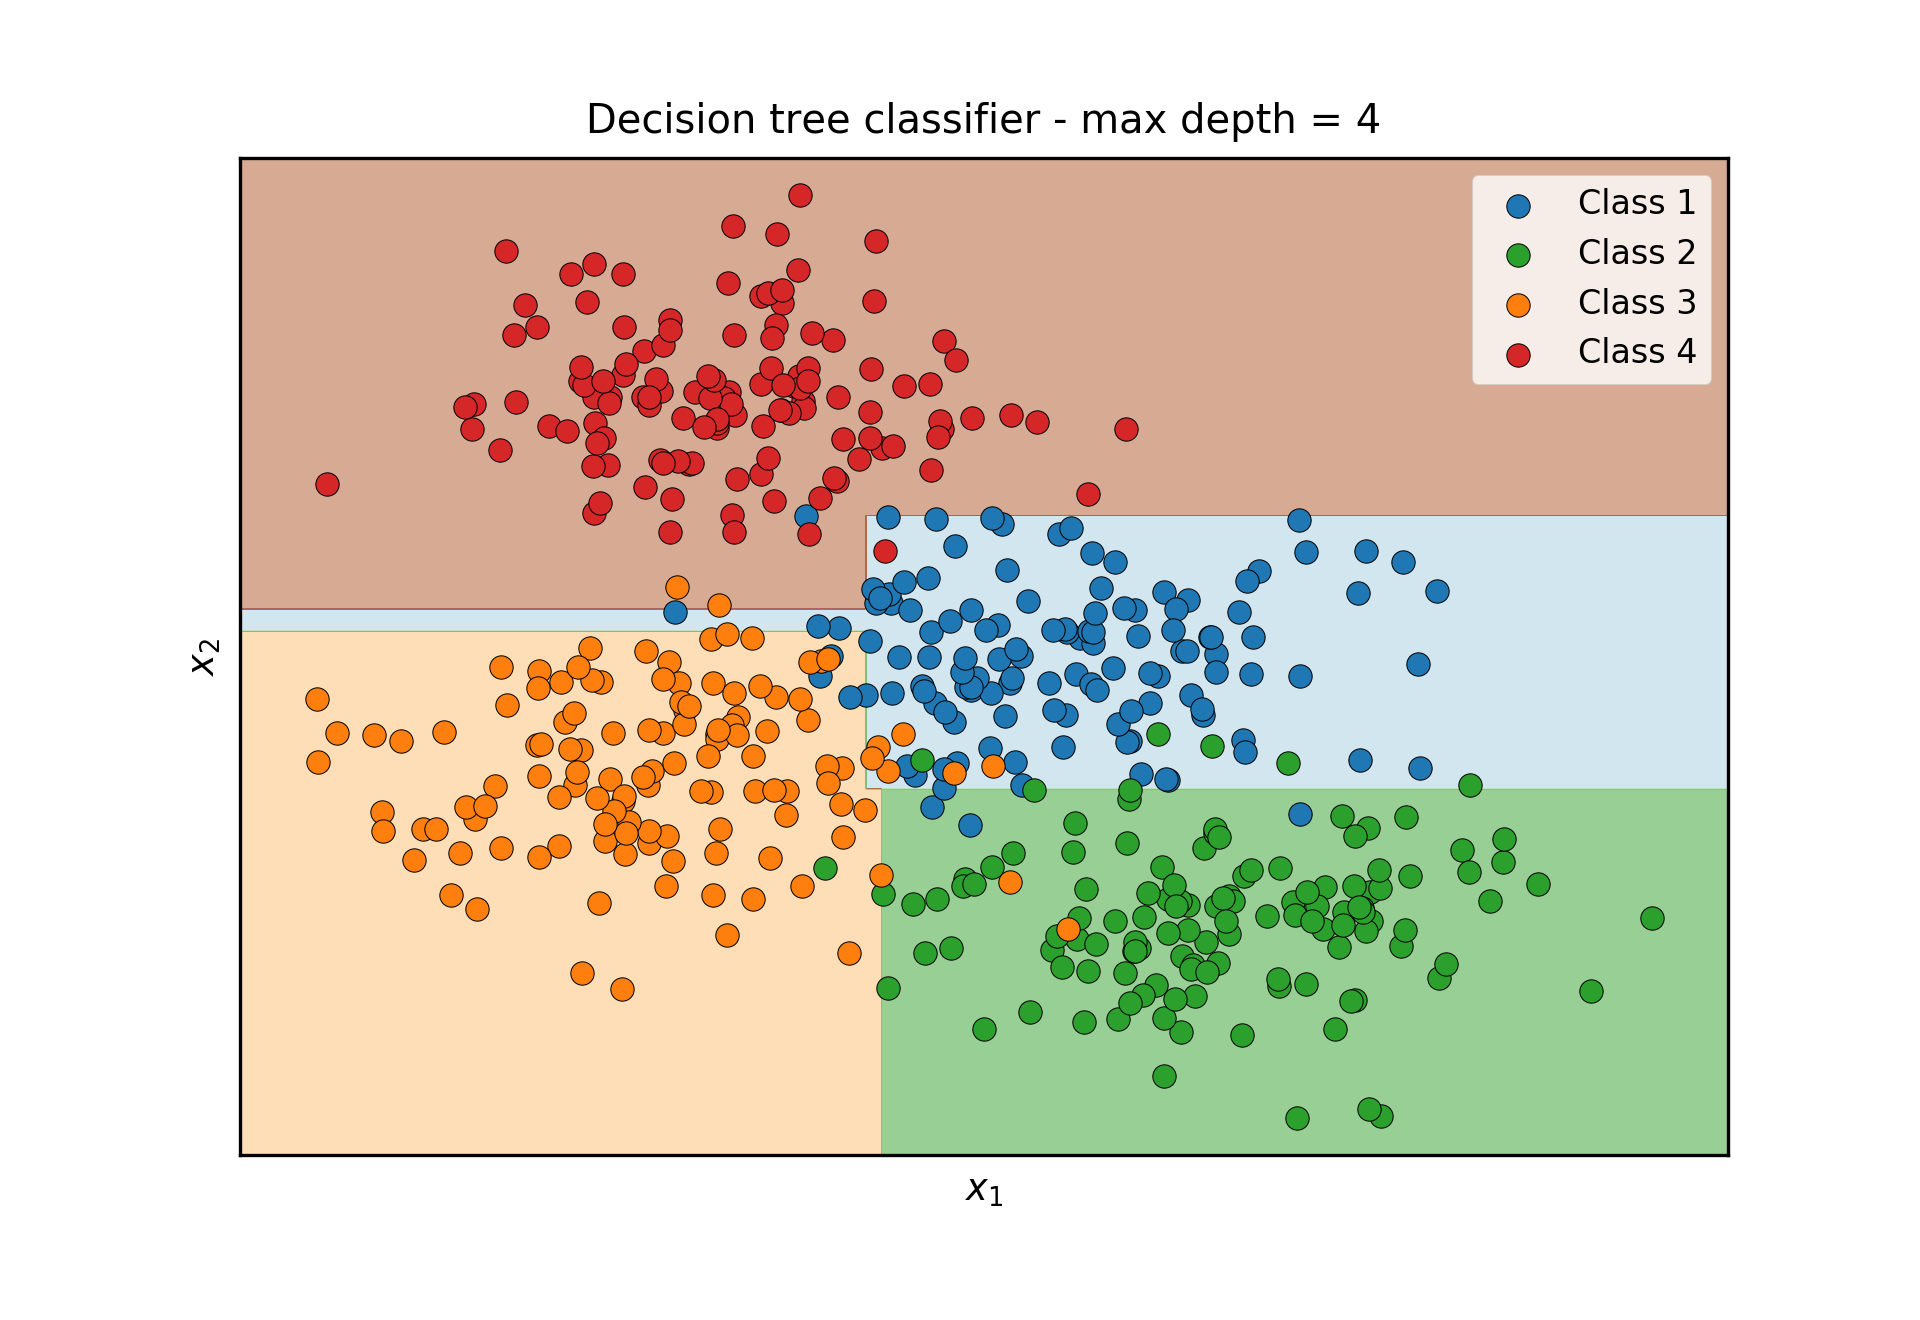
\includegraphics[width=0.5\textwidth]{part1/decsion_tree_classification.png}
				\label{fig:dt_clf}%
			}%
			%			\hfill%
			\subfloat[]{%
				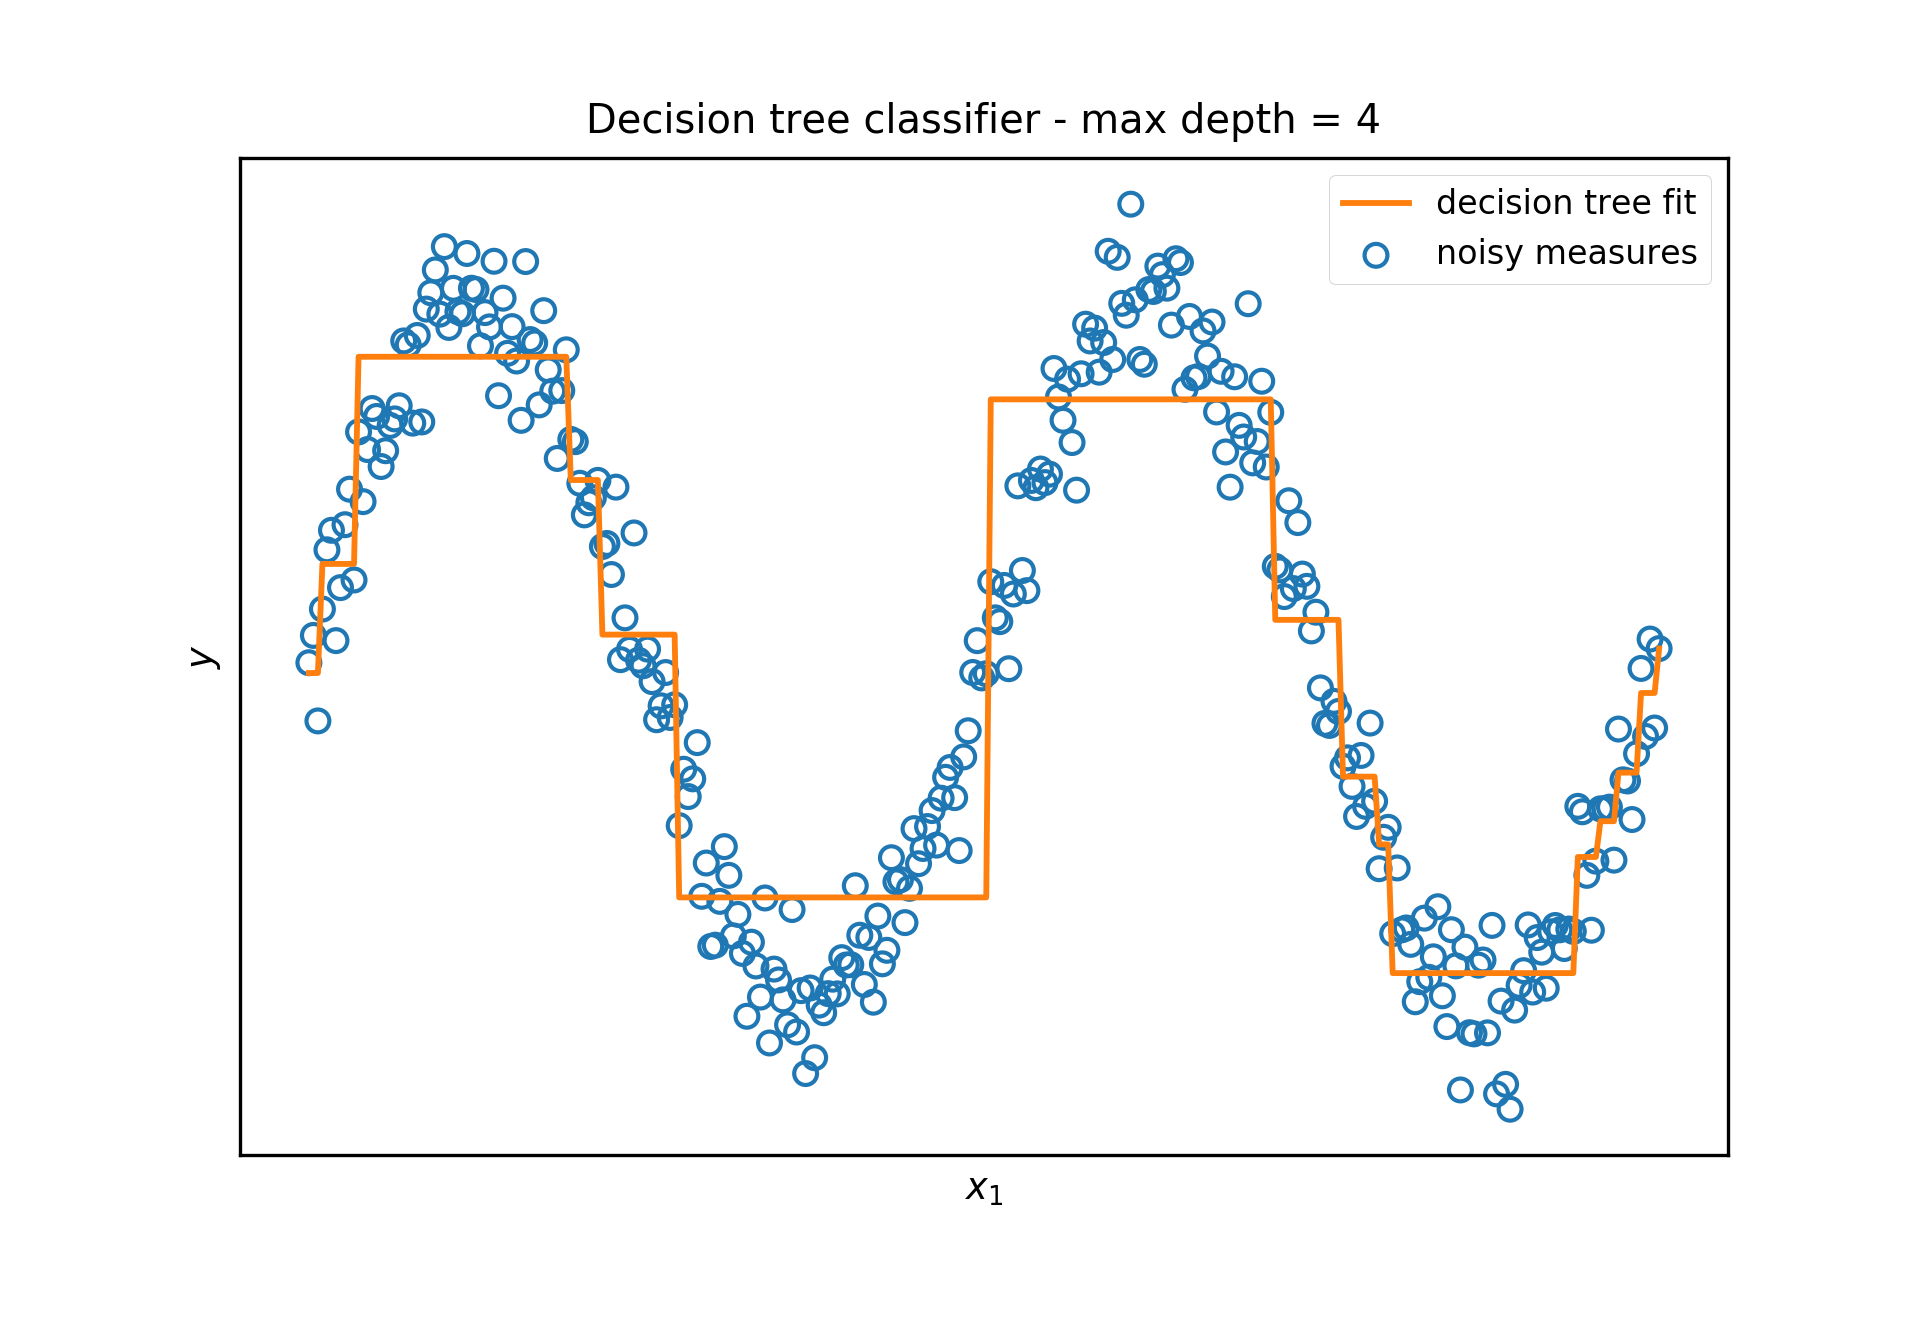
\includegraphics[width=0.5\textwidth]{part1/decsion_tree_regression.png}
				\label{fig:dt_rgr}%
			}%
			\caption{Two examples of decision tree applications for: (a) 2D multiclass classification problem, (b) 1D regression problem.}\label{fig:decision_trees}
		\end{figure}
		
		Fitting a decision tree implies learning from the data the structure of the tree itself, including the selection of the input variable for each splitting recursion, as well as the optimal splitting threshold. Moreover, it must also be defined the value of the prediction for each region.
		Let's take into account the usual setting: $\mathcal{D} = \{(\bm{x}_i, y_i)\}_{i=1}^n = (X, \bm{y})$. Even when the number of nodes is fixed, defining at the same time: which variables to split, their splitting threshold and the predictive value is computationally unfeasible as it has a combinatorially large number of possible solutions. Therefore, starting from the root note, \ie the whole input space, and fixing a maximum tree depth, we resort to a greedy approximation.
		
		Let the data at the node $m$ be denoted by $Q_m$, then for each candidate split $\theta=(j, s_m)$, consisting of the $j^{\text{th}}$ feature and the threshold $s_m$, we define two half-planes as follows.
		$$
		Q_{m_1}(\theta) = (\bm{x}_i, y_i) | \bm{x}_i^j \leq s_m~\text{and}~Q_{m_2}(\theta) = (\bm{x}_i, y_i) | \bm{x}_i^j > s_m
		$$
		Then, at each node an impurity measure is evaluated using a suitable impurity function $H(Q_m)$, which depends on the given task. Therefore, we can formulate an objective function like
		$$
		J(Q_m,\theta) = \frac{n_1}{n_m}H(Q_{m_1}(\theta)) + \frac{n_2}{n_m}H(Q_{m_2}(\theta))
		$$
		where $n_1$ and $n_2$ is the number of samples in region $Q_{m_1}$ and $Q_{m_2}$, respectively, while $n_m=n_1+n_2$.
		For each node we then select the best parameter solving the optimization problem in Equation~\eqref{eq:CART}.
		\begin{equation} \label{eq:CART}
			\hat \theta_m = \argmin_{\theta} J(Q_m,\theta)
		\end{equation}
		This procedure is recursively applied to $Q_{m_1}(\hat \theta_m)$ and $Q_{m_2}(\hat \theta_m)$ until the maximum tree depth, that we have fixed at the beginning, is reached.
		
		Dealing with regression problems, a typical impurity measure can be, for instance, the Mean Squared Error (\ac{MSE})
		\begin{equation} \label{eq:MSE}
			H_{\text{MSE}}(Q_m) = \frac{1}{n_m} \sum_{\bm{x}_i \in R_m} \big(y_i - \bar y_m \big)^2
		\end{equation}
		where $\bar y_m = \frac{1}{n_m} \sum_{\bm{x}_i \in R_m} y_i$, is the average output of $Q_m$, \ie the training samples in region $R_m$;
		or the Mean Absolute Error (\ac{MAE})\footnote{we previously came across this measure when evaluating the performance of learning methods on the aging problem, see Sections~\ref{sec:ols},~\ref{sec:ridge_regression},~\ref{sec:the_lasso}, \etc.}, which is simply defined as below.
		\begin{equation} \label{eq:MAE}
				H_{\text{MAE}}(Q_m) = \frac{1}{n_m} \sum_{\bm{x}_i \in R_m} | y_i - \bar y_m |
		\end{equation}
		On the other hand, dealing with (multiclass) classification problems, where the classes are identified by the index $k=1,\dots,K$, typical impurity measures are, for instance, the Gini criterion
		\begin{equation} \label{eq:gini}
			H_{\text{Gini}}(Q_m) = \sum_{k=1}^K p_{mk}(1-p_{mk})
		\end{equation}
		where $p_{mk}=\frac{1}{n_m} \sum_{\bm{x_i} \in R_m} \mathds{1}(y_i = k)$ is the proportion of class $k$ observation on the region $R_m$; or the Cross-Entropy (\ac{CE})
		\begin{equation} \label{eq:ce}
			H_{\text{CE}}(Q_m) = - \sum_{k=1}^K p_{mk} \log(p_{mk})
		\end{equation}
		which is an impurity measure heavily also applied as loss function for other  learning machines (see Appendix~\ref{appendix:A}).
		
		The main free parameter of this model is the maximum depth of the tree, \ie its size. Deeper trees are capable of modeling complex input-output relationships with respect to shallow ones. Obviously, too deep trees can overfit the training data. Therefore, the optimal depth of the tree should be estimated from the data via, for instance, grid-search cross-validation.
				
		Decision trees are important in biomedical data science applications as they are easily interpretable and capable of modeling nonlinear input-output relationships. Indeed, the prediction is given following a number of binary decisions which, in some cases, may mimic the way doctors perform diagnosis on their patients. Relatively small decision trees can actually be represented graphically. For instance, applying a this method to the aging problem presented in Section~\ref{sec:ols}, we obtain the tree shown in Figure~\ref{fig:tree_graph}. As usually, the main free parameter of the model, \ie the maximum depth of the tree,  is chosen via grid-search cross-validation (and it is $3$, in this case).
		
		\begin{figure}[!hb]
			\centering
			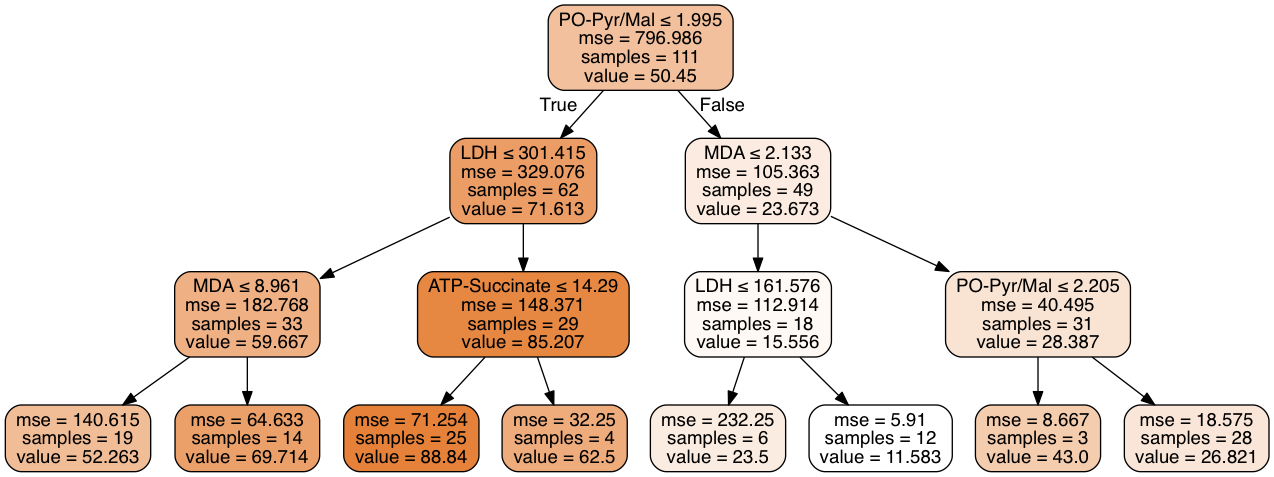
\includegraphics[width=0.8\textwidth]{part1/decsion_tree_graph.png}
			\caption{The graph structure learned from the aging problem (see Section~\ref{sec:ols}). The maximum depth of the tree is $3$ and it is chosen via grid-search cross-validation.} \label{fig:tree_graph}
		\end{figure}
	
		A very well-known weakness of decision trees is their instability. In fact, decision trees are not robust to noise affecting the input data. Even minor perturbations of a single feature may generate a different split which propagates down to all the splits below. In practice, this is alleviated by the use of decision trees as base learners of ensemble strategies (see Section~\ref{sec:ensemble_methods}).
		More details on this learning paradigm and its applications can be found reading~\cite{hastie2009elements}, Chapter 9 or~\cite{bishop2006pattern}, Chapter 14.

		%%%%%%%%%%%%%%%%%%%%%%%%%%%%%%%%%%%%%%%%%%%%%%%%%%%
	    \subsection{Ensemble methods} \label{sec:ensemble_methods}
	    The key idea of ensemble methods is to build a prediction model by aggregating a collection of multiple \textit{base learners} that are trained to solve the same problem~\citep{zhou2012ensemble}.

	    % FIXME
	    \textit{Bagging} is a common ensemble strategy that consists in fitting multiple models $f_b(\bm{x})$ for $b=1,\dots,B$ each one on a \textit{bootstrap} sampling\footnote{random sampling with replacement} $\mathcal{D}_b$ of the training dataset  $\mathcal{D}=\{\bm{x}_i, y_i\}_{i=1}^n$.
%	    \citep{hastie2009elements}
	    For each sample $\bm{x}_i$, the bagging estimate $\hat{f}(\bm{x}_i)$ is obtained by combining the predictions of the base learners $\hat{f}_b(\bm{x}_i)$. For instance, in case of classification tasks, the bagged model may select the most predicted class casting a vote among the $B$ base learners. On the other hand, for regression problems, the bagging estimate can be a (weighted) mean, or the median, of the predictions of the $B$ base learners. Decision trees (see Section~\ref{sec:decision_trees}) are typical base learner for bagged estimators.

	    % FIXME
	    \textit{Boosting} is another popular ensemble strategy that, unlike bagging, performs predictions by sequentially fitting a collection of base learner that cast a weighted vote~\citep{hastie2009elements}. At each boosting step, the weight corresponding to samples that were misclassified at the previous iterations increases. Therefore, each successive classifier is somewhat forced to learn the relationships between input and output that were previously missed. From a theoretical standpoint, it would be possible to boost any learning machine, nevertheless boosting methods are mainly used with decision trees as base learners~\cite{hastie2009elements}.

		%%%%%%%%%%%%%%%%%%%%%%%%%%%%%%%%%%%%%%%%%%%%%%%%%%%%%%%%%%%%%%%%%%
	    \subsubsection{Random Forests} \label{sec:random_forests}
%	    Decision trees are easily interpretable models that recursively partitions the training data into subsets, based on the test of a single feature value at each split (or node). At each iteration, the feature that yields the best split in terms of a pre-selected metric (Gini impurity, information gain or variance reduction) is chosen to create a new node. Decision trees is that they tend to not perform well in practice, which led to the introduction of random forests in 2001~\cite{breiman2001random}.

	    Random Forests (\ac{RF}) are ensembles of decision trees, proposed by Leo Breiman in the early 2000s~\cite{breiman2001random} to ameliorate the instability of decision trees.
	    In RF each tree is grown on a bootstrap sample from the training data, typically to its maximum depth.
	    To increase robustness to noise and diversity among the trees, each node is split using the best split among a subset of features randomly chosen at that node. The number of features on which the trees are grown is one of the free parameters of the model.
	    The final prediction is made by aggregating the prediction of $M$ trees, either by a majority vote in the case of classification problems, or by averaging predictions in the case of regression problems.
	    Another important free parameter of the model is the number of trees in the ensemble.
	    RF are a bagging approach, which works on the assumption that the variance of individual decision trees can be reduced by averaging trees built on many uncorrelated subsamples.
	    Moreover, increasing the number of trees in the ensemble, RF does not overfit the data. Therefore, this parameter is typically chosen to be \textit{as large as possible}, consistently with the available hardware and computational time.
%	    By contrast, {\it boosted decision trees} are made by building an iterative collection of decision trees, trained by giving more importance to training examples that were incorrectly classified by the previous trees. \todo{Add use cases for boosted decision trees. $\dots$}

	    RF can provide several measures of \textit{feature importance}, computed by looking at the increase in prediction error % (mean decrease in accuracy; mean decrease in node impurity)
	    when data for a feature is permuted while all other features remain unchanged. 
	    Feature selection based on random forests if most often performed using one of these measures. However, several techniques for applying regularization to random forests have been proposed. These techniques broadly fall under two categories:
	    \begin{enumerate}
			\item cost-complexity pruning, which consists in limiting tree depth, resulting in less complex models~\cite{ishwaran2008random,kulkarni2012pruning}; and
			\item Gini index penalization~\cite{deng2013gene, liu2014learning}.
	    \end{enumerate}
    	In addition,~\cite{joly2012ell1} proposed using an $\ell_1$-norm  to reduce the space-complexity of random forests.

	    RF naturally handle both numerical and categorical variables, multiple scales, and non-linearities. They also require little parameter tuning. This makes them popular for the analysis of diverse types of biological data, such as gene expression, Genome-wide Association Studies (\ac{GWAS}) data or mass spectrometry~\cite{qi2012random}.
		In practice, feature selection schemes that rely on RF may to be unstable~\cite{kursa2014robustness}, therefore feature selection stability measures must be adopted to avoid drawing inconsistent conclusions.
		
		Let's see what happens when RF are applied to the aging problem (see Section~\ref{sec:ols}). The experimental setup is identical to the one previously applied for ridge and Lasso regression (see Section~\ref{sec:ridge_regression} and~\ref{sec:the_lasso}), where the only parameter optimized via grid-search cross-validation is the maximum number of features each tree can grow on (and in this case it is chosen as $4$). The number of trees in the ensemble is fixed to $500$. The RF model on the test set achieves $\text{MAE} = 6.321$ and Explained Variance $\text{EV} = 88.17\%$.
		Figure~\ref{fig:rf_feature_importance} shows the feature importance measure estimated by this model.
		\begin{figure}[!h]
			\centering
			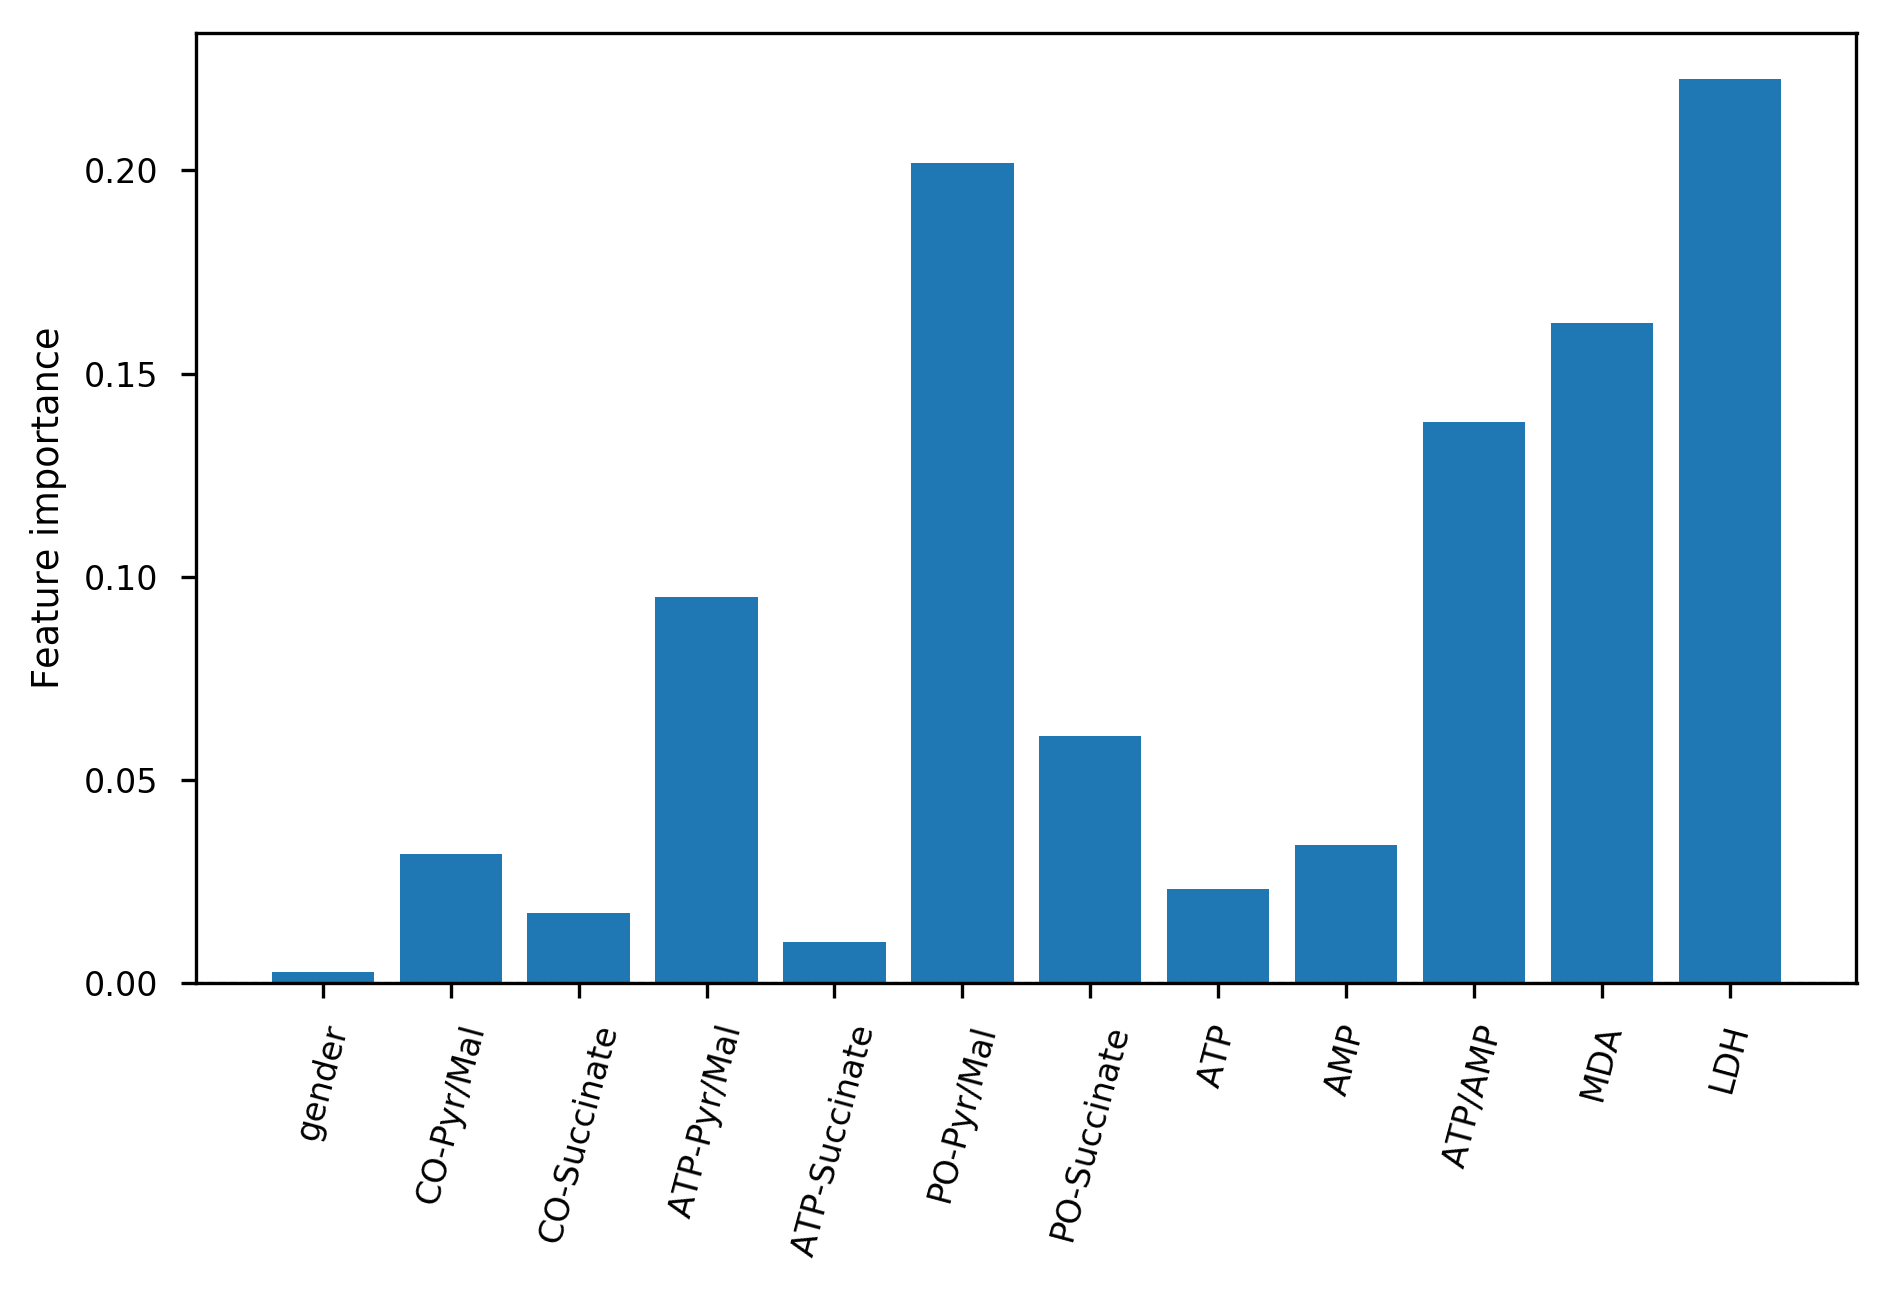
\includegraphics[width=0.8\textwidth]{part1/rf_feature_importance.png}
			\caption{A pictorial representation of the feature importance achieved by a RF model with $500$ trees growing on $4$, out of $12$, features.} \label{fig:rf_feature_importance}
		\end{figure}
		As we can see, the features that are most relevant for RF are comparable to the ones selected by Elastic-Net (see Figure~\ref{fig:w_enet}).
		For RF models it is interesting to investigate on the effect of an increasing value for the number of trees in the forest. As shown in Figure~\ref{fig:rf_increasing}, increasing the number of trees in the forest does not lead to overfit. In fact, test error (Figure~\ref{fig:rf_mae}) and explained variance (Figure~\ref{fig:rf_ev}), after approximately $400$ trees, reach a plateau region instead of growing.
	    \begin{figure}[!h]
			\centering
			\subfloat[]{%
				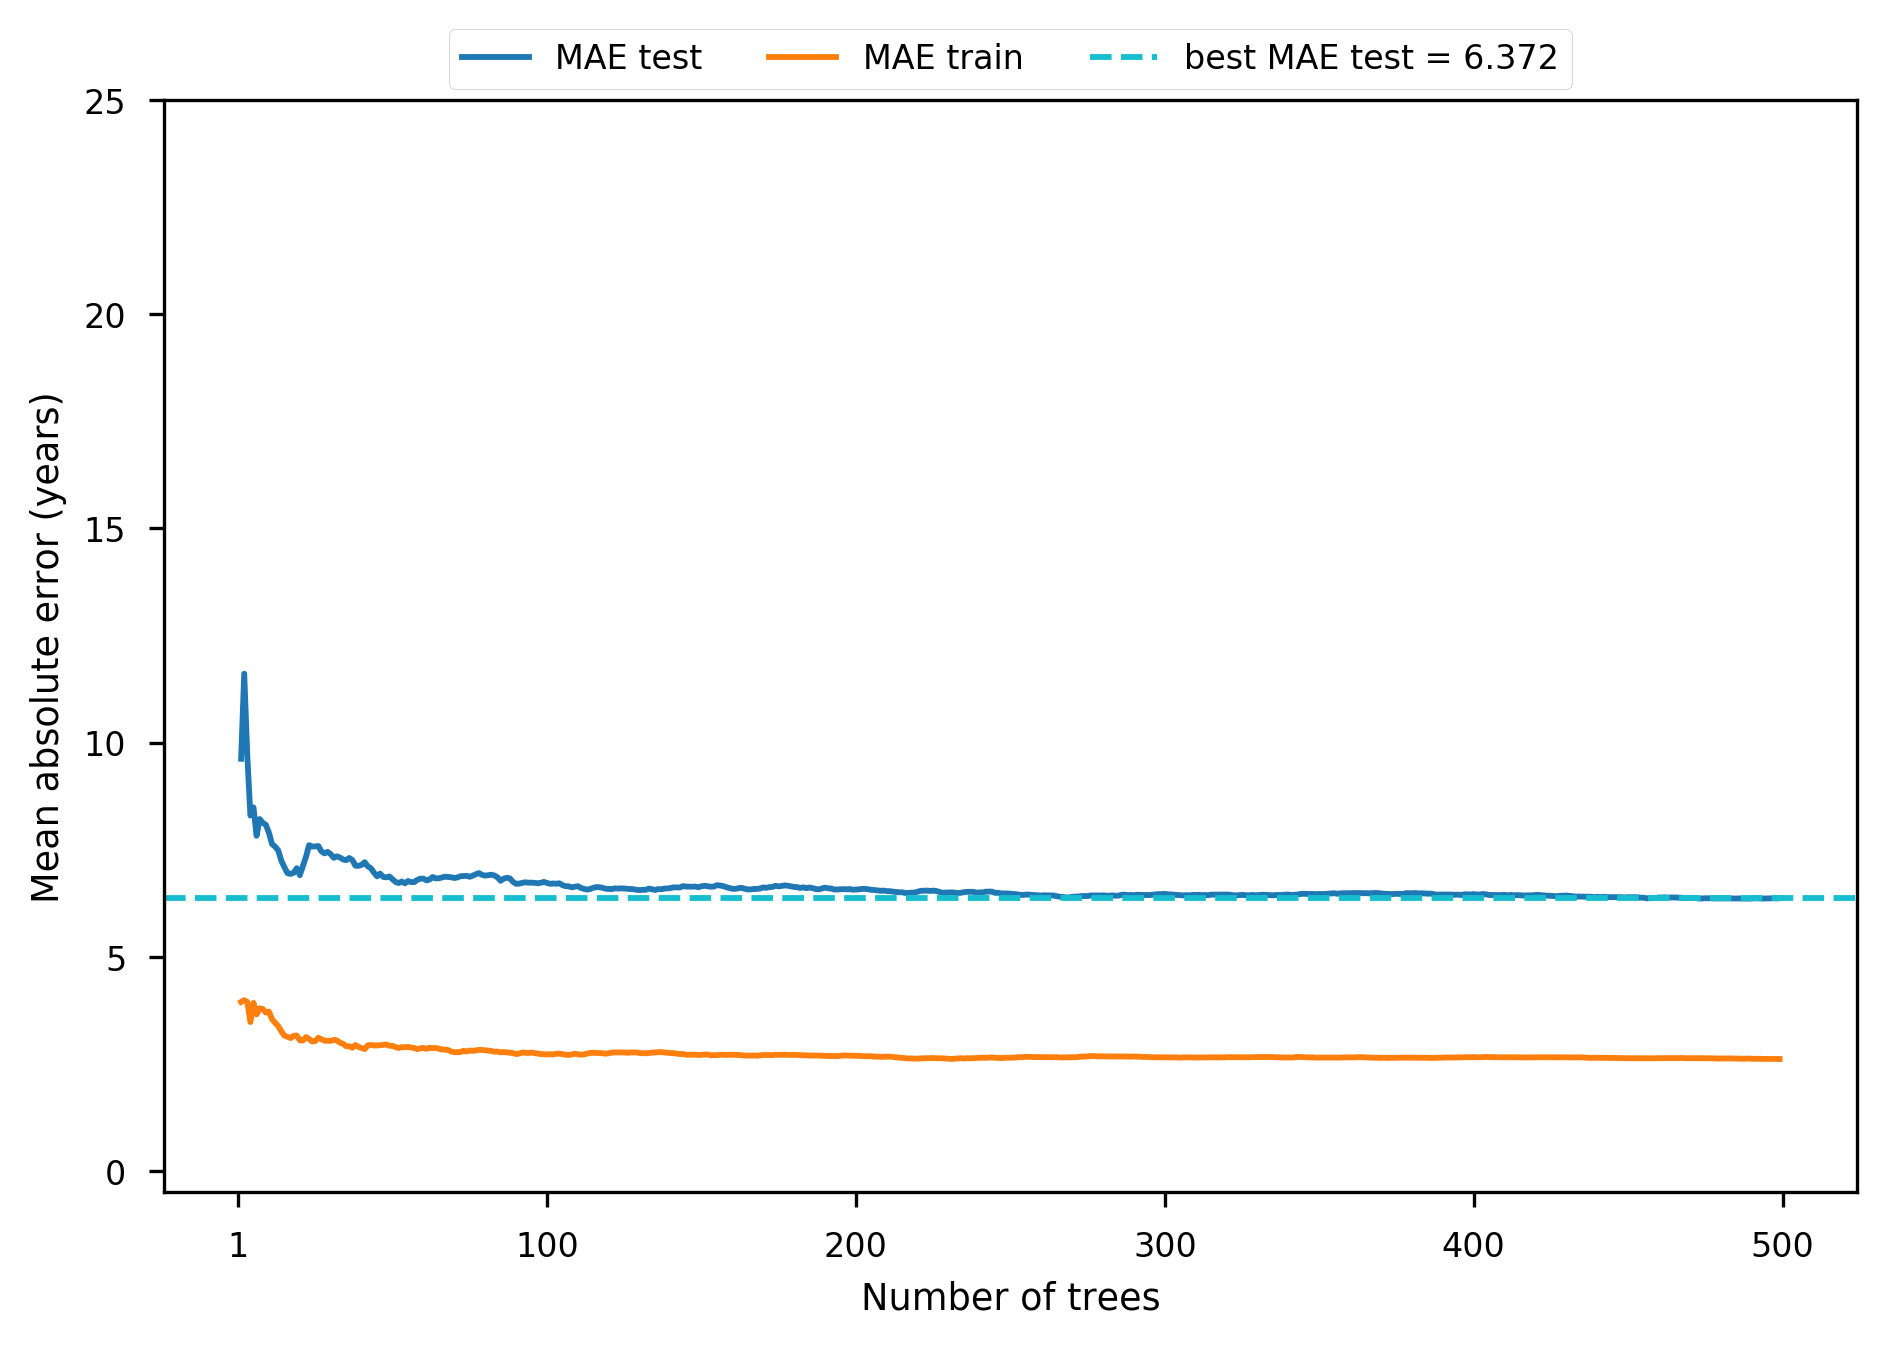
\includegraphics[width=0.5\textwidth]{part1/rf_increasing_MAE.png}
				\label{fig:rf_mae}%
			}%
			%			\hfill%
			\subfloat[]{%
				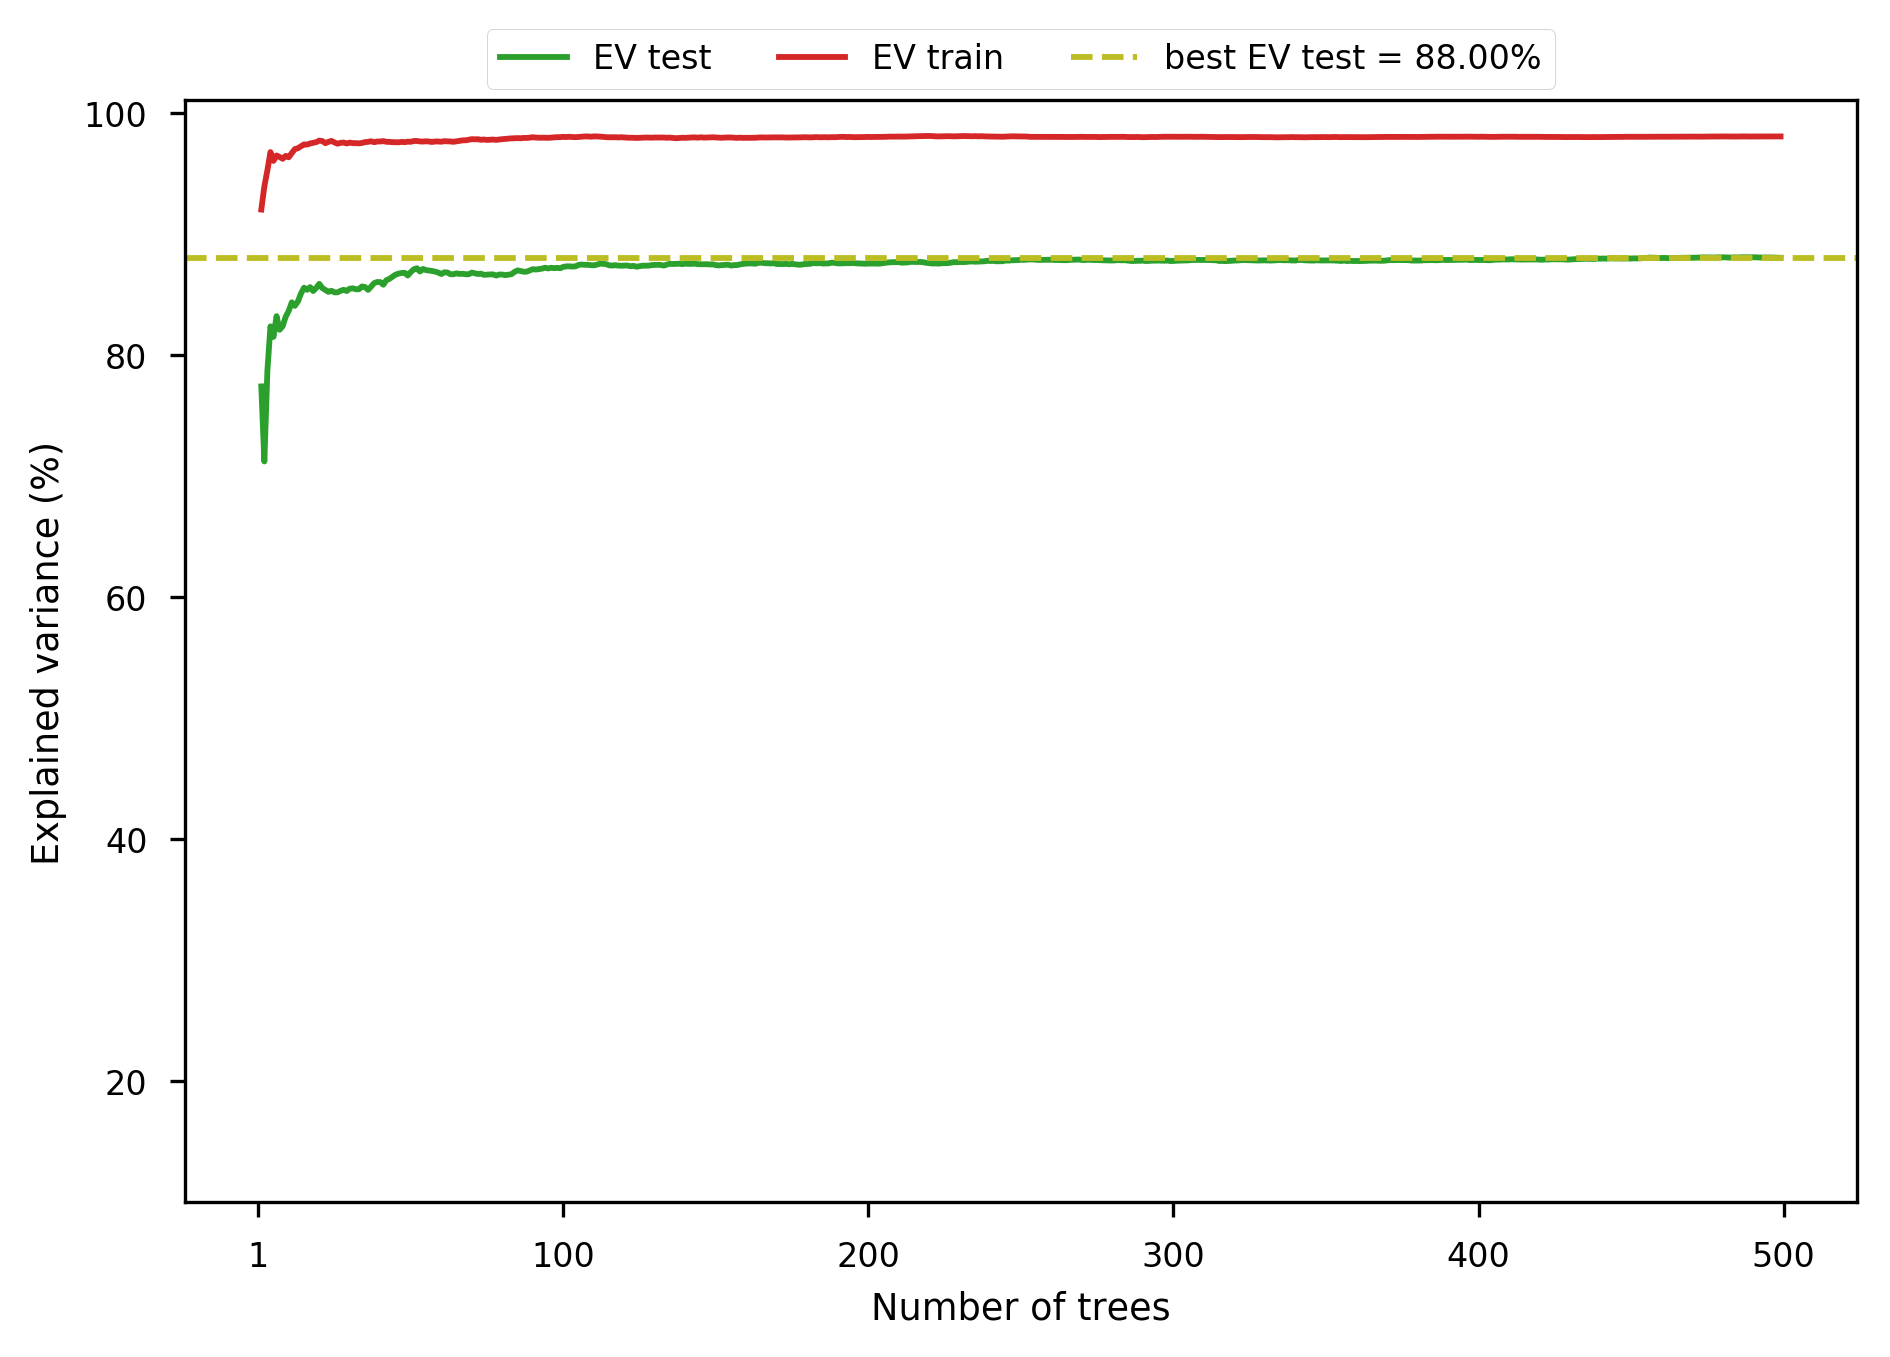
\includegraphics[width=0.5\textwidth]{part1/rf_increasing_EV.png}
				\label{fig:rf_ev}%
			}%
			\caption{The effect of the number of trees in a RF model in terms of MAE, panel (a), and EV, panel (b). As expected, larger forests do not lead to overfit, \ie the training error does not reach zero.}\label{fig:rf_increasing}
		\end{figure}

		%%%%%%%%%%%%%%%%%%%%%%%%%%%%%%%%%%%%%%%%%%%%%%%%%%%%%%%%%%%%%%%%%%%%%%
	    \subsubsection{Gradient Boosting} \label{sec:gradient_boosting}
	    
	    \textit{Gradient boosting}~\cite{friedman2001greedy} (\ac{GB}) is one of the most widely applied boosting methods in biological problems.
	    This technique iteratively combines the predictions obtained by several base learners, such as decision trees, into a single model.
	    The key idea behind GB is that, under some general hypothesis on the cost function, boosting can be seen as an iterative gradient method for numerical optimization.
	    In particular, in GB at each boosting iteration a new base learner is fitted on the residuals obtained at the previous boosting iteration.
	    GB has several desirable properties~\cite{mayr2014evolution}, such as its capability to learn nonlinear input-output relationship, its ability to embed a feature importance measure (as RF) and its stability in case of high-dimensional data~\cite{buehlmann2006boosting}. When used for feature selection, GB shows interesting performance when casted in the stability selection framework~\cite{meinshausen2010stability}, leading to an effective control of the false discovery rate.

	    As for most of the learning machine, GB may suffer of overfitting. The main regularization parameter to control is the number of boosting iterations $M$, \ie the number of base learners, fitted on the training data. This is typically optimized by cross-validated grid-search, or by information criteria-based heuristics~\cite{tutz2006generalized, tutz2007boosting}.
	    Regularization in GB can also be controlled by shrinking the contribution of each base learner by a constant $0<\nu<1$ that controls the learning rate of the boosting procedure. In order to achieve comparable predictive power, smaller values of $\nu$ imply larger number of $M$, so there is a trade-off between them.
	    As usually the base learners are decision trees and another important parameter to tune is their maximum depth~\cite{hastie2009elements}.

	    In a recent paper~\cite{lusa2015boosting}, the authors show that in high-dimensional balanced binary classification problems, if the base learner is likely to overfit the training data, the use of \textit{Stochastic GB}~\cite{friedman2002stochastic} is preferable. The latter is a modified version of the original method, where each base learner is fitted on a random extraction without resubmission of a fraction $\eta$ of the training data, where $\eta$ is another regularization parameter to choose.
	    
	    Let's see what happens when GB is used to tackle the aging problem (see Section~\ref{sec:ols}).
	    The experimental setup is identical to the one previously applied for Elastic-Net regression (see Section~\ref{sec:elastic_net}), where the two parameters optimized via grid-search cross-validation are the maximum depth (in a range from $3$ to $20$) of the trees and the number of boosting iterations (with a maximum value of $500$).
	    The selected tree depth is $8$ and the number of boosting iterations is $31$.
		The GB model on the test set achieves $\text{MAE} = 7.955$ and Explained Variance $\text{EV} = 84.88\%$.
	    Figure~\ref{fig:gb_feature_importance} shows the feature importance measure estimated by this model.
	    \begin{figure}[!h]
	    \centering
	    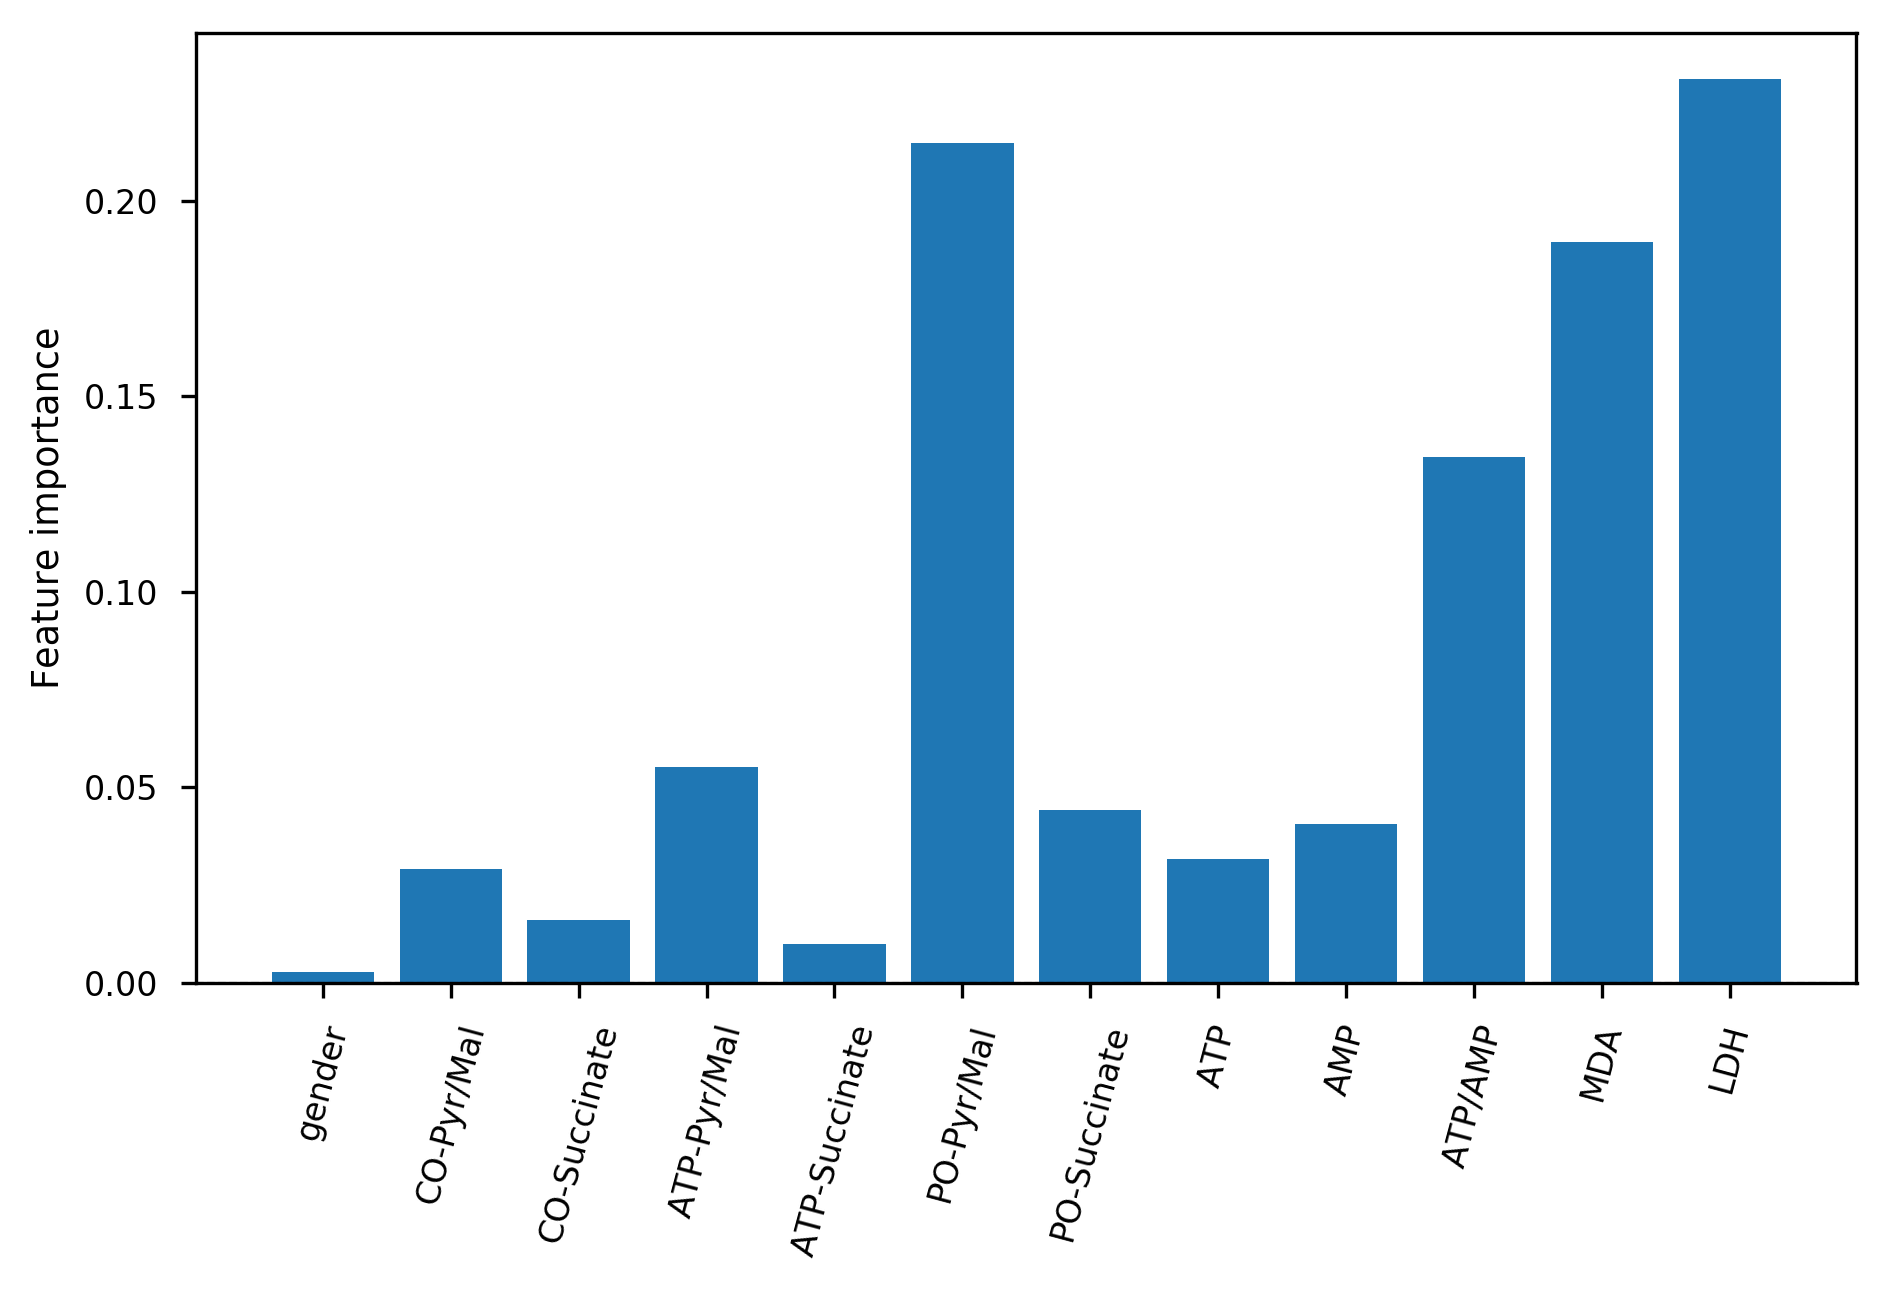
\includegraphics[width=0.8\textwidth]{part1/gb_feature_importance.png}
    	\caption{A pictorial representation of the feature importance achieved by a GB model with learning rate $0.1$ after $31$ boosting iterations. Each tree has maximum depth of $11$ and it grows on $4$, out of $12$, features.} \label{fig:gb_feature_importance}
	    \end{figure}
   		As we can see, the features that are most relevant for GB are comparable to the ones relevant for RF (see Figure~\ref{fig:rf_feature_importance}).
	    As we have already seen for RF, we shall investigate on the effect of increasing boosting iterations for GB. As shown in Figure~\ref{fig:gb_increasing}, after approximately $50$ boosting iterations the model reaches perfect overfit of the training set, \ie zero training error (Figure~\ref{fig:gb_mae}) and $100\%$ trained explained variance (Figure~\ref{fig:gb_ev}).
        \begin{figure}[!h]
    	\centering
    	\subfloat[]{%
    		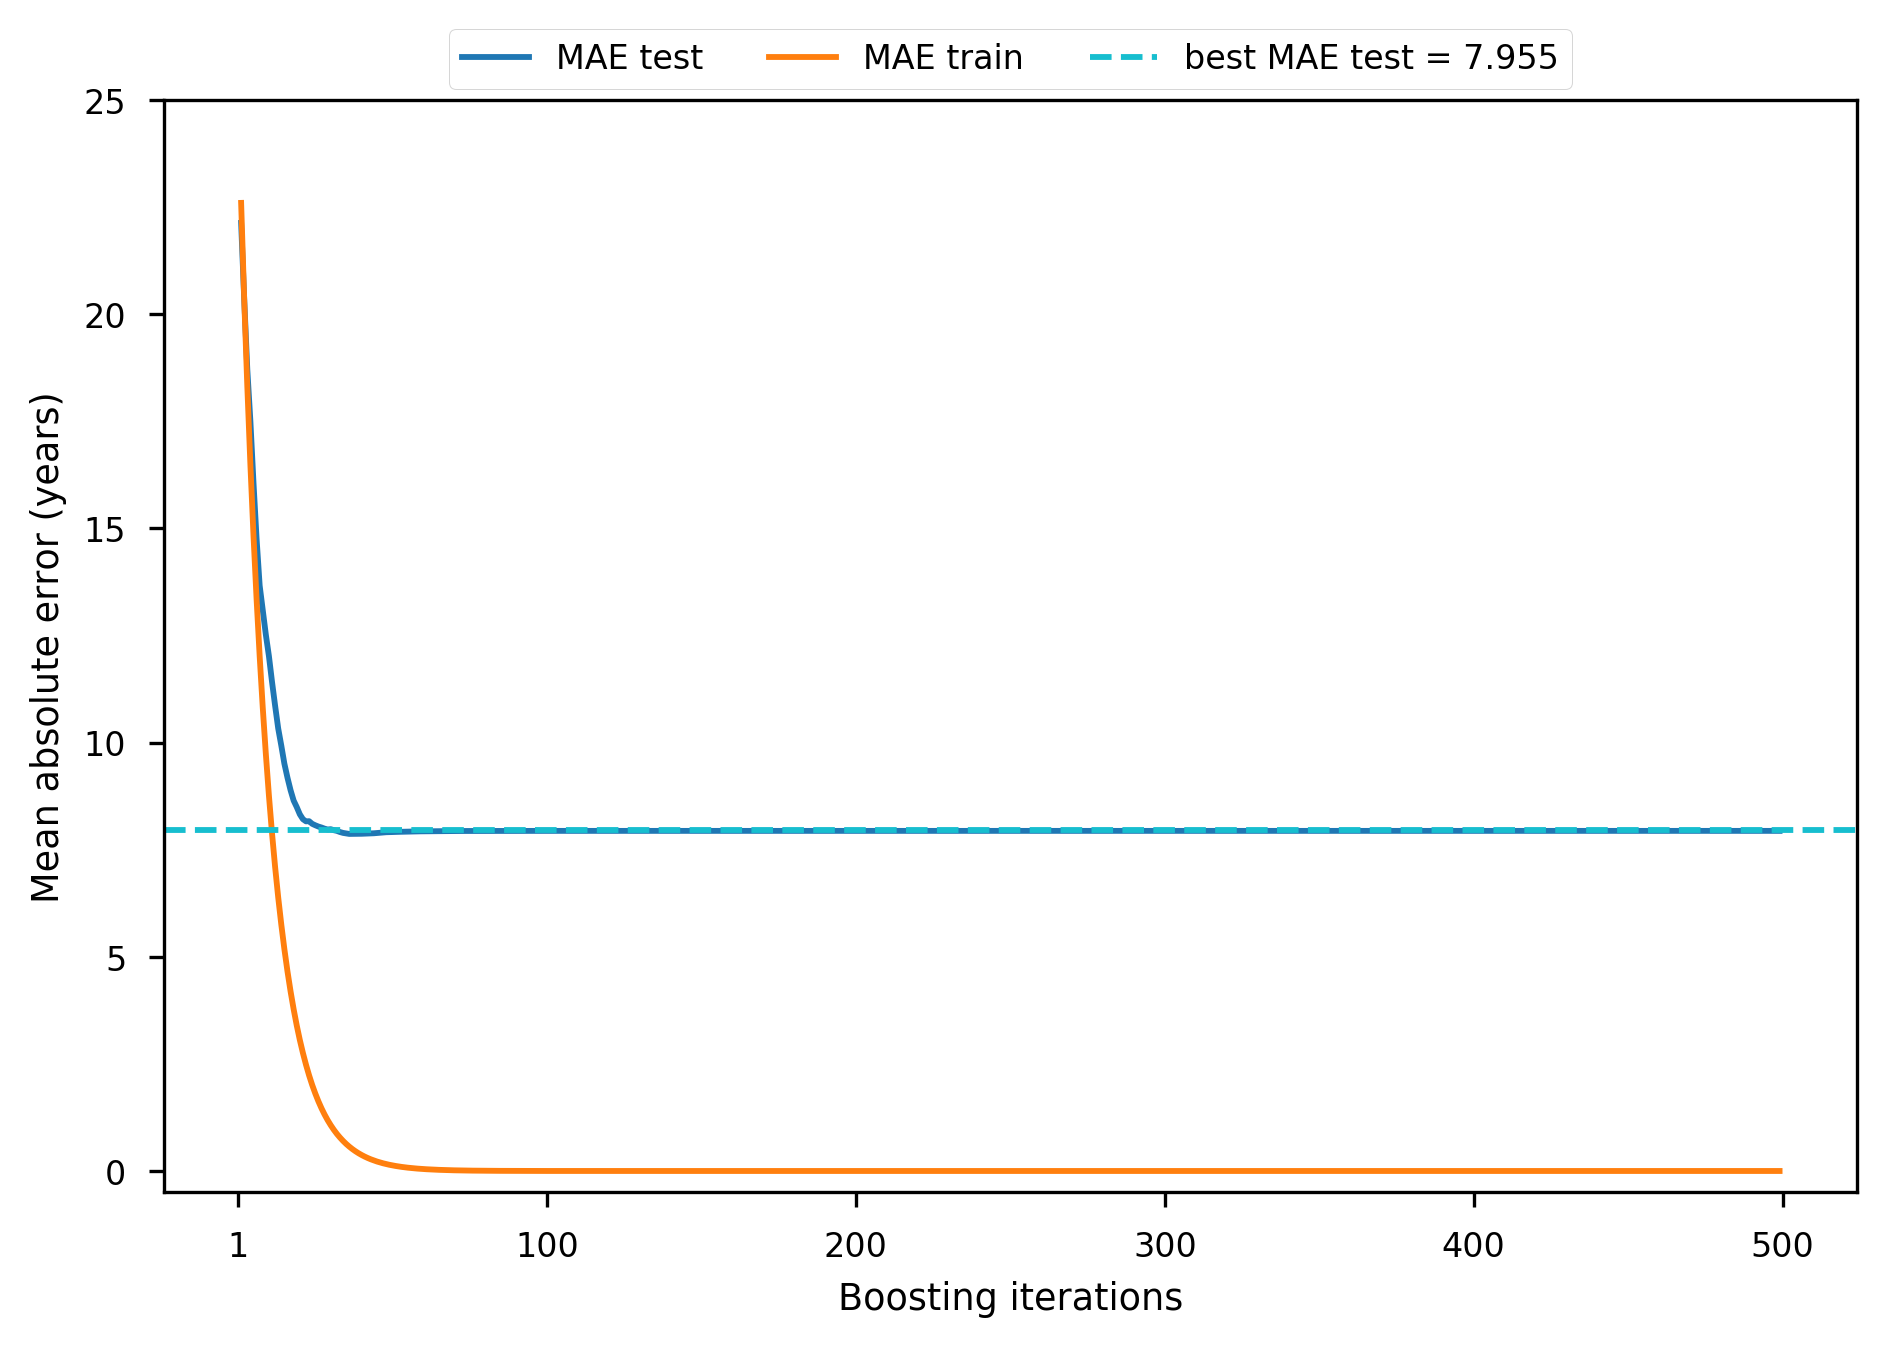
\includegraphics[width=0.5\textwidth]{part1/gb_increasing_MAE.png}
    		\label{fig:gb_mae}%
    	}%
    	%			\hfill%
    	\subfloat[]{%
    		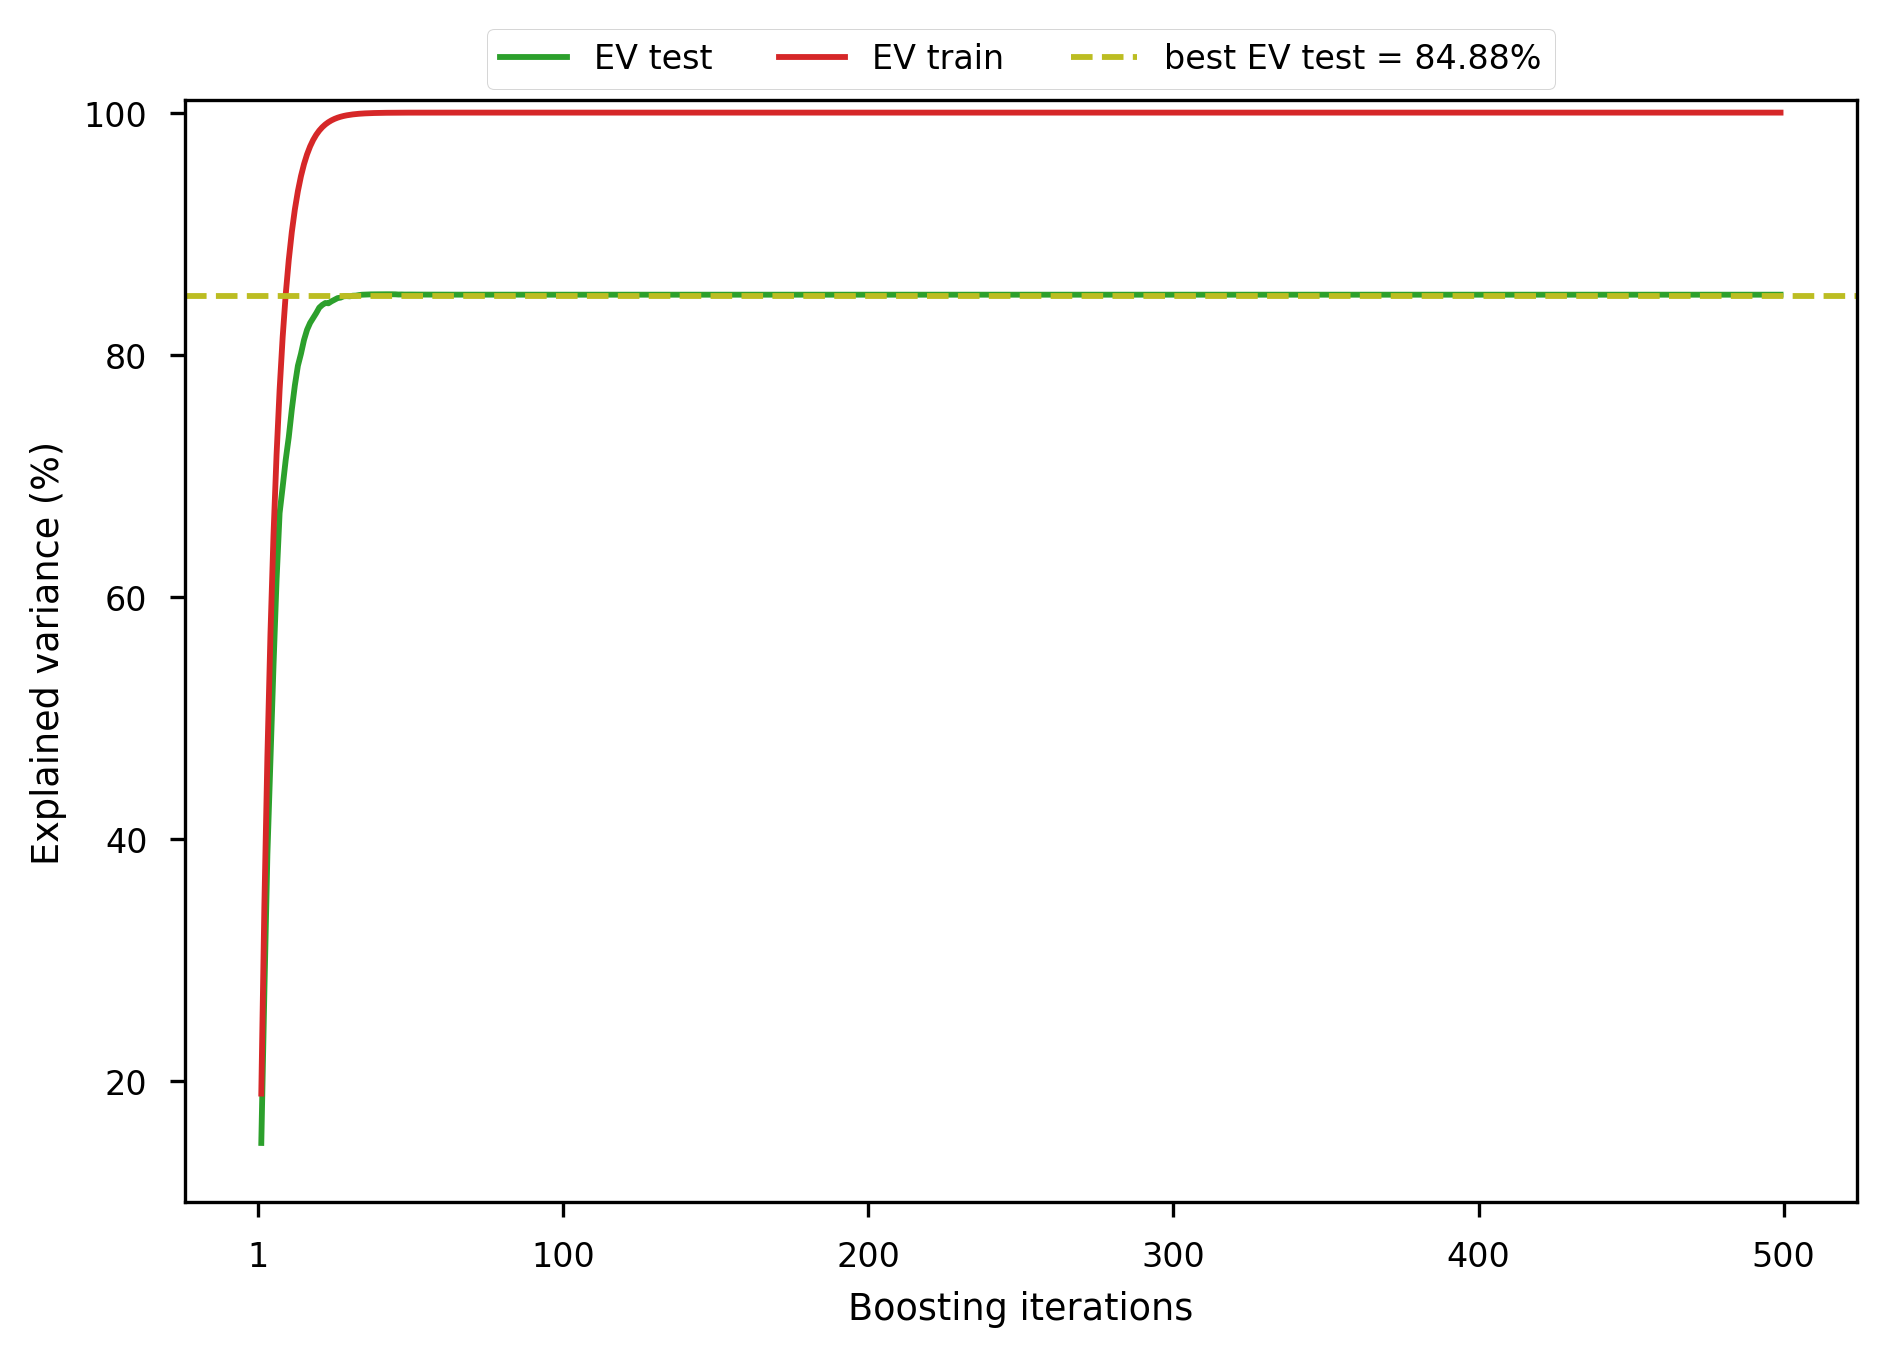
\includegraphics[width=0.5\textwidth]{part1/gb_increasing_EV.png}
    		\label{fig:gb_ev}%
    	}%
    	\caption{The effect of the number of boosting iterations in a GB model (learning rate $0.1$) in terms of MAE, panel (a), and EV, panel (b). As expected, increasingly large boosting iterations lead to perfect overfit, \ie zero training error.}\label{fig:gb_increasing}
	    \end{figure}
	    

%	    Approaches based on gradient boosting classification are used to detect \textit{de novo} mutations showing an improved specificity and sensitivity with respect to state-of-the-art methods~\cite{liu2014gradient}.
%	    When combined with stability selection~\cite{meinshausen2010stability}, gradient boosting has demonstrated to be a very resourceful method for variable selection, leading to an effective control of the false discovery rate. This strategy was followed to associate overall survival with single-nucleotide polymorphisms of patients affected by cutaneous melanoma~\cite{he2016component} and to detect differentially expressed amino acid pathways in autism spectrum disorder patients~\cite{hofner2015controlling}.

%	    \todo{consider adding boosting method for cox models...}

		%%%%%%%%%%%%%%%%%%%%%%%%%%%%%%%%%%%%%%%%%%%%%%%%%%%%%%%%%%%%%%%%%
	    \subsection{Deep learning}
	    
		Deep Learning (DL) is a branch of ML that, in the recent past, is becoming extremely appealing thanks to the high predictive power that it has empirically shown on real-world problems.
		This section is definitely not an attempt to summarize the heterogeneous plethora of the DL methods presented in literature so far. Indeed, even a dedicated PhD thesis may not be enough to accomplish this task.
		In this section we will only get a grasp on the mechanisms behind the supervised DL methods applied in Part II\footnote{unsupervised DL methods are available as well, but as they are not used in Part II, their discussion is not presented here. We recall to~\cite{lecun2015deep, goodfellow2016deep, chollet2018deep} for a more comprehensive overview.}.
	    
	    % I shall not forget that this is Regularization in bio studies, there are plenty of ML in bio studies out there
	    One of the main characteristics of DL methods is that, starting from raw data, they aim at learning a suitable feature representation (see Section~\ref{subsec:unsupervised_learning}) and a prediction function, at the same time.
	    DL methods stand on the shoulders of the classical, and shallow, Neural Networks of the $80$s, and they can actually be seen as their extension.
	    In DL the the final prediction is achieved by composing several layers of non-linear transformations.
	    The intuition behind DL method is that, starting from raw data, their multi-layer architecture can achieve representations at a more abstract level, leading to top performance in prediction tasks.
	    DL architectures can be devised to tackle binary or multiclass classification~\cite{angermueller2016deep, leung2014deep} as well as single or multiple output regression~\cite{Chen2016GeneEI, ma2015deep} tasks.
	    %\todo{microarray gene xpression multi-task regression }

		\subsubsection{Multi-Layer Perceptron} \label{sec:mlp}
		In order to understand the principles guiding DL methods, we sketch here the ideas behind the most basic one: the Multi-Layer Perceptron (\ac{MLP}), also known as deep Feedforward Neural Network.
	    Typically, MLPs are structured as fully connected graphs organized in \textit{layers} that can be of three different types: \textit{input}, \textit{hidden} and \textit{output} (see Figure~\ref{fig:mlp}).
	    Each node of the graph is called \textit{unit}.
	    The number of units in the input layer matches the dimensionality of the raw data ($d$), while number and type of output units are related to the learning task.
	    For multiclass classification problems, with $K$ classes, the output layer has $K$ units, each one representing the probability of the input sample to be assigned to one specific class.
	    On the same line, for multiple-output regression problems, with $K$ tasks, each one of the $K$ unit corresponds to the prediction for a given task.
	    Size and number of the hidden layers can be arbitrarily chosen according to prediction task and available computational resources.
	    
   	    \def\layersep{2.0cm}

\begin{figure}
	\caption{A pictorial representation of the structure of a Multi-Layer Perceptron example with two hidden layers having four and three hidden units, respectively. According to the nature of the output layer, this network topolgy can be adopted either for regression or binary classification problems starting from raw samples in a two-dimensional space.} \label{fig:mlp}
	\centering
	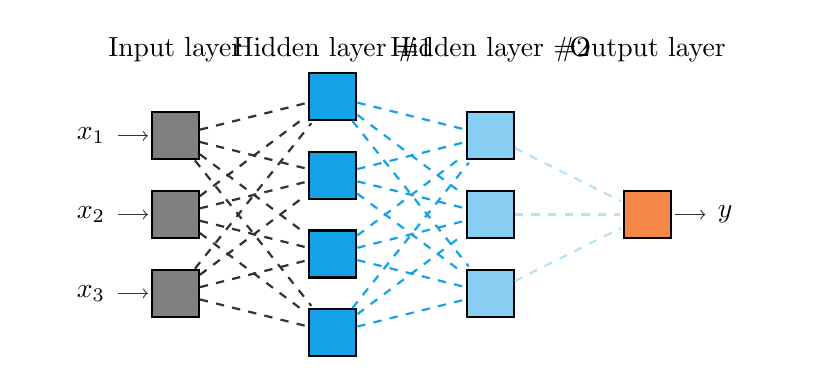
\begin{tikzpicture}[shorten >=1pt,-, draw=black!80, node distance=\layersep]
	\tikzstyle{every pin edge}=[<-,shorten <=1pt]
	\tikzstyle{neuron}=[draw=black, thick, rectangle, minimum size=17pt, inner sep=0pt, thick]
	% \tikzstyle{neuron}=[square, minimum size=17pt, inner sep=0pt, thick]
	\tikzstyle{input neuron}=[neuron, fill=Gray];
	\tikzstyle{output neuron}=[neuron, fill=Peach];
	\tikzstyle{hidden neuron}=[neuron, fill=Cerulean];
	\tikzstyle{hidden neuron2}=[neuron, fill=Cerulean!50];
	\tikzstyle{annot} = [text width=10em, text centered]


	% Draw the input layer nodes
	\foreach \name / \y in {1,...,3}
	% This is the same as writing \foreach \name / \y in {1/1,2/2,3/3,4/4}
	\node[input neuron, pin=left:$x_\y$] (I-\name) at (0,-\y) {};

	% Draw the hidden layer nodes
	\foreach \name / \y in {1,...,4}
	\path[yshift=0.5cm]
	node[hidden neuron] (H-\name) at (\layersep,-\y cm) {};

	% Draw the hidden layer nodes
	\foreach \name / \y in {1,...,3}
	\path[yshift=0.0cm]
	node[hidden neuron2] (H2-\name) at (\layersep+\layersep,-\y cm) {};

	% Draw the output layer node
	\node[output neuron,pin={[pin edge={->}]right:$y$}, right of=H2-2] (O) {};

	% Connect every node in the input layer with every node in the
	% hidden layer.
	\foreach \source in {1,...,3}
	\foreach \dest in {1,...,4}
	\path (I-\source) edge[thick,-,dashed] (H-\dest);
	% \path[path fading=fade IH1, thick, dashed, draw=Gray] (I-\source) -- (H-\dest);


	\foreach \source in {1,...,4}
	\foreach \dest in {1,...,3}
	\path (H-\source) edge[thick,-,dashed,draw=Cerulean] (H2-\dest);
	% \path[path fading=fade H1H2, thick, dashed, draw=Gray] (H-\source) -- (H2-\dest);

	% Connect every node in the hidden layer with the output layer
	\foreach \source in {1,...,3}
	\path (H2-\source) edge[thick,-,dashed,draw=Cerulean!30] (O);
	% \path[path fading=fade H2O, thick, dashed, draw=Gray] (H2-\source) -- (O);

	% Annotate the layers
	\node[annot,above of=H-1, node distance=0.6cm] (hl) {Hidden layer \#1};
	\node[annot,right of=hl] (hl2) {Hidden layer \#2};
	\node[annot,left of=hl] {Input layer};
	\node[annot,right of=hl2] {Output layer};
	\end{tikzpicture}
\end{figure}

	    
	    In MLPs the information flows through the graph from the input to the output.
	    Each layer $l$ transforms its input data $\bm{x}^{l-1}$ by composing an affine transformation and an activation function $\sigma(\bm{x})$ that acts element-wise on its input vector.
	    In other words, defining as $p_{l-i}$ the number of units in the layer $l-i$, the layer $l$ applies the transformation
	    $$
	    \bm{x}^{l} = \sigma(\bm{x}^{(l-1)}W_l+b_l)
	    $$
	    where $W_l \in \mathbb{R}^{p_{l-1} \times p_l}$ and $\bm{b} \in \mathbb{R}^{p_l}$ are the weights of the model that are learned from the data.
	    
	    The function $\sigma(\bm{x})$ is known as \textit{activation function} and it can be defined in different ways.
	    In classical neural networks, activation functions are modeled as sigmoids (\eg $\sigma(x)=\tanh(x)$, $\sigma(x)=(1+e^{-x})^{-1}$) whilst in modern DL architectures the most used activation function is the Rectified Linear Unit: $f(x)=\max(0,x)$.
	    % \begin{equation}\label{eq:relu}
	    % 	f(\bm{x})=\begin{cases} 0  &\text{for}~~  x <0 \\ x  &\text{for~}~x \geq 0 \end{cases}
	    % \end{equation}

	    % \todo{output layers + regularization + works}
	    Particular attention must be paid when fitting deep models as they can be prone to overfit the training set~\cite{angermueller2016deep}.
	    The network topology itself defines the \textit{degrees of freedom} of the model: deeper and wider networks can approximate well very complicated input-output relationship, but also the noise affecting the data.
	    Although, tuning the number of hidden layers and their size is not the recommended strategy to prevent from overfitting, as it may lead to suboptimal solutions.

	    Regularization in MLPs can be controlled by penalizing the weights of the network. A common regularization strategy consists in adding an $\ell_2$-norm penalty in the objective function, as in Equation~\eqref{eq:losspen}. In the DL community this procedure is known as weight decay~\cite{krogh1992simple}.
	    Although less common, the $\ell_1$-norm can also be adopted as regularization penalty, as in~\cite{leung2014deep}.
%	    This strategy is adopted in \cite{Chen2015TransspeciesLO} to train a deep architecture on rat cell responses to given stimuli with the final aim to predict human cell responses in the same conditions.
%	    Moreover, weight decay is also adopted in \cite{Yuan2016DeepGeneAA} to train \textit{DeepGene}, \ie an MLP which is designed to classify the tumor type from a set of somatic point mutations.
%	    Furthermore, weight decay is used in~\cite{Fakhry2016DeepMF} to train a DL architecture for brain electron microscopy image segmentation.
	    
	    Training MLPs, and deep networks in general, consists in solving a minimization problem via suitable optimization algorithms~\cite{ruder2016overview}. All these methods iteratively update the weights of the network in order to decrease the training error. Another fundamental regularization strategy is the \textit{Early stopping}~\cite{prechelt1998early}. This consists in interrupting the fitting process as soon as the error on an external validation set increases~\cite{angermueller2016deep}.

	    Another common regularization strategy in DL is \textit{Dropout}~\cite{srivastava2014dropout}. This techniques consists in temporarily deactivating a defined number of randomly chosen units of the network at training phase. This reduces the degrees of freedom of the model and it implicitly allows to achieve an ensemble of several smaller networks whose predictions are combined.
	    The use of dropout alone can improve the generalization properties, as in~\cite{Chen2016GeneEI}, but it is usually adopted in combination with weight decay or other forms of regularization, as in~\cite{leung2014deep}.
	    
	    Training MLP may imply dealing with non-convex optimization problems which are usually tackled via stochastic gradient descend, or similar methods~\cite{ruder2016overview, sra2012optimization}.
%	    , where the authors propose to use a deep network to predict splicing patterns.
%	    where the authors propose a \textit{D-GEX}, DL regression architecture trained to predict the expression of a number of target genes. Dropout

		MLP architectures are also used as final layers of another class of DL methods called: Convolutional Neural Network (\ac{CNN}).
		CNN are a different class of DL methods that exploit convolutional masks with weights estimated from the data to learn a suitable feature representation. This class of methods is largely applied to computer vision and image recognition problems.
		Describing CNN architectures is beyond the scope of this thesis, as they are not mentioned in the Part II. A thorough description of CNN can be found here~\cite{goodfellow2016deep}.

		Let's see what happens when a relatively simple MLP is applied to the aging problem (see Section~\ref{sec:ols}). The experimental setup is the same used for RF in Section~\ref{sec:random_forests}, where the only parameter optimized via grid-search cross-validation is the weight decay constant.
		The resulting MLP has $1$ hidden layer with $1024$ units, ReLu activation and weight decay constant $0.001$.
		Such MLP is trained with early stopping and, after $XX$ iterations reaches $\text{MAE} = 9.14$ explaining the $78.84\%$ of the variance of the test set.
		The relatively worse performance of this method, compared, for instance, to RF, may be due to the fact that this dataset has a reduced number of samples. It is known that DL methods, in order to reach optimal solutions, need more training samples than conventional learning machines.
		
		\subsubsection{Long-Short Term Memory Network} \label{sec:lstm}
		Long-Short Term Memory Network (LSTM) belongs to the class of Recurrent Neural Network (\ac{RNN})~\cite{goodfellow2016deep}.
		LSTM use special units, called {\sl memory cells}, which have the ability to learn long-term dependencies \cite{lecun2015deep}. 
		Instead of just applying an element-wise nonlinear function, such as sigmoid or hyperbolic tangent, to the affine transformation of inputs and recurrent units.
		LSTM cells have an internal self-loop together with a system of {\sl input}, {\sl output} and {\sl forget gates}~\cite{goodfellow2016deep}.
		Compared to standard RNNs, LSTMs can be trained via gradient descent as they do not suffer from the vanishing/exploding gradient problem~\cite{bengio1994learning}.
		In the recent past, this deep learning architectures demonstrated to achieve promising results in several sequences learning tasks, such as speech recognition~\cite{graves2005framewise}, image captioning~\cite{vinyals2015show}, or time-series forecast~\cite{schmidhuber2005evolino}. 
		
  \section{Feature selection} \label{subsec:feature_selection}

  \section{Unsupervised learning} \label{subsec:unsupervised_learning}
  In Section~\ref{subsec:supervised_learning} we started the discussion of supervised learning methods with a metaphorical comparison with the human ability of learning from examples.
  Actually, in order to understand some concept, human beings need way less supervision than modern learning algorithms.
  In some circumstances it may be even the case that little/no supervision at all is needed to accomplish a task.
  For instance, let's say that a kid growing with a Brittany dog at home visit some friend having a Bernese Mountain Dog.
  The kid, so far, has only being taught what his dog looks like and these two dog breeds definitely look different one another.
  Nevertheless, the kid will certainly be able to understand that both of them are animals and, in particular, dogs.
  Who taught the kid the appearance of every possible dog breed?
  
  The learning paradigm in which we try to infer some interesting properties, or recurrent patterns from unlabeled samples is known as unsupervised learning.
  Quoting Kevin P. Murphy: "\textit{Unsupervised learning is arguably more typical of human and animal learning}."~\cite{murphy2012machine}.
  
  In this section, given a set of input data $\mathcal{D}=\{\bm{x}_i\}_{i=1}^n$, with samples represented as $d$-dimensional vectors $\bm{x}_i \in \mathbb{R}^d$ ($\forall i=1,\dots,n$), our interest will be directed toward two different goals:
  \begin{enumerate*}[label=(\roman*)]
  	\item grouping similar objects together (Section~\ref{sec:clustering}) and
  	\item achieving a meaningful low-dimensional representation of our data (Section~\ref{sec:dimred}).
  \end{enumerate*}
  In both cases we will try to infer the properties of the probability distribution $p(\bm{x})$ from which the collected data are assumed to be drawn.
  
    \subsection{Cluster analysis} \label{sec:clustering}
    \textit{Cluster analysis}, \aka \textit{data segmentation} or \textit{clustering}, is the class of unsupervised learning algorithm which aim at grouping together similar objects, by some definition of \textit{similarity}.
        
    This task is fairly common in biomedical studies, where cluster analysis can be used, for instance, to perform patients stratification or to find groups of correlated biological measures, such as gene expression, blood exams, and so on. This section presents an overview on the most popular clustering algorithms.\footnote{a good reference for the clustering algorithms proposed in literature is section \textit{2.3. Clustering} of the \sklearn documentation \url{http://scikit-learn.org/stable/modules/clustering.html}.}

    \subsubsection{The $k$-means algorithm} \label{sec:k-means}
    $k$-means is the most intuitive strategy for cluster analysis.
    
%    It is basically what $k$-nearest neighbor and OLS are for supervised classification and regression, respectively.
	Given $n$ samples $\bm{x}_i \in \mathbb{R}^d$, the goal of $k$-means partitions the data space into $K$ non-overlapping groups containing similar samples.
    Let $\bm{\mu}_k \in \mathbb{R}^d$ be the \textit{prototypical} vector associated with the $k^{\text{th}}$ cluster, we can think of this as the center of mass of the cluster, \ie its centroid.
    Fixed the number of cluster $K$, the output of the $k$-means algorithm is a set of cluster centroids as well as the assignment of each sample to a single cluster.
    For ease of notation, we introduce a binary indicator function $r_k$ defined as
    $$
 	r_k(\bm{x}_i)=\begin{cases} 1  &\text{if}~\bm{x}_i~\text{is assigned to cluster}~k \\ 0  & \text{otherwise} \end{cases}
    $$
    (this is known as 1-of-$K$ encoding). Therefore, we can define the objective function
    $$
    J(\bm{\mu}) = \sum_{i=1}^n\sum_{k=1}^K r_k(\bm{x}_i) d(\bm{x}_i, \bm{\mu}_k)
    $$
    where $d(a,b)$ is some distance measure. In case $d(a,b)$ is the squared Euclidean distance, which is the typical choice for $k$-means, the objective function can be rewritten as in Equation~\eqref{eq:kmeans}.
    \begin{equation} \label{eq:kmeans}
    J(\bm{\mu}) = \sum_{i=1}^n\sum_{k=1}^K r_k(\bm{x}_i) \norm{\bm{x}_i- \bm{\mu}_k}_2^2
    \end{equation}
    Our goal is to find the centroids $\bm{\mu}_k$ for $k=1,\dots,K$ that minimize $J(\bm{\mu})$.
    We may observe that, given the best centroids, the samples will be associated to the cluster with the nearest centroid. So, let's focus on the problem of finding $\bm{\mu}_k$.
    Fixing $r_k(\bm{x})$ for all $k$, the objective function in Equation~\eqref{eq:kmeans} is quadratic in $\bm{\mu}$, thus the minimization problem can be easily solved setting its derivative to zero, see Equation~\eqref{eq:kmeans_solved}.
    \begin{equation} \label{eq:kmeans_solved}
	2\sum_{i=1}^n r_k(\bm{x}_i)(\bm{x}_i - \bm{\mu}_k) = 0 \Rightarrow \bm{\mu}_k = \frac{\sum_{i=1}^n r_k(\bm{x}_i)\bm{x}_i}{\sum_{i=1}^nr_k(\bm{x}_i)}
    \end{equation}
    Intuitively, $\bm{\mu}_k$ corresponds to the mean of the points assigned to the cluster $k$.
    The $k$-means algorithm starts with random centroids. Then, the points are assigned to the cluster having the nearest centroid. Successively, the centroids position is updated. At each step the value of $J(\bm{\mu})$ is reduced, hence the convergence of $k$-means is assured. Nevertheless, the algorithm may converge to a local minimum, achieving a suboptimal solution.
    
    For a given dataset, defining an optimal value for $K$ is still an open problem. The $k$-means algorithm works with a number of cluster fixed a priori\footnote{some relevant work on automatic cluster discovery is presented in~\cite{ball1967clustering, pelleg2000x, muhr2009automatic}}.
    This is be given from some prior knowledge on the problem, or it can be estimated following some heuristics. Otherwise, an estimate of $K$ can be defined by optimizing data-driven coefficients like the silhouette score~\cite{rousseeuw1987silhouettes}, or some information criteria, such as \ac{AIC} or \ac{BIC}~\cite{bishop2006pattern}.
    These estimates can be done with or without cross-validation~\cite{fiorini2017adenine}.
    
    As shown in~\cite{arthur2007k}, smart choices of the initial position of the clusters can substantially improve the result. For instance the initial $\bm{\mu}_k$, for $k=1,\dots,K$, can be chosen to be \textit{far away} from each other.
    This solution is called $k$-means$++$ and it follows the steps summarized below.
%    \begin{enumerate}
%    	\item choose the first centroid $\bm{\mu}_1$ at random from the samples in the dataset;
%    	\item compute the distance between $\bm{\mu}_1$ and all the other points in the dataset: $D = d(\bm{x}_i, \bm{\mu}_1)$ $\forall i=1,\dots,n$;
%    	\item choose a new data point as centroid $\bm{\mu}_2$ following a weighted probability distribution $\propto~D^2$;
%    	\item update the distance vector as $D = \min[d(\bm{x}_i, \bm{\mu}_1), d(\bm{x}_i, \bm{\mu}_2)]$ $\forall i=1,\dots,n$;
%    	\item repeat steps 3 and 4 until $k$ centroids are defined;
%    	\item use this centroids initialization to run standard $k$-means.
%    \end{enumerate}

	\begin{algorithm}[h!]
		\begin{algorithmic}[1]
			\State choose the first centroid $\bm{\mu}_1$ at random from the samples in the dataset
			\State compute the distance between $\bm{\mu}_1$ and all the other points in the dataset: $D = d(\bm{x}_i, \bm{\mu}_1)$ $\forall i=1,\dots,n$
			\State choose a new data point as centroid $\bm{\mu}_2$ following a weighted probability distribution $\propto~D^2$
			\State update the distance vector as $D = \min[d(\bm{x}_i, \bm{\mu}_1), d(\bm{x}_i, \bm{\mu}_2)]$ $\forall i=1,\dots,n$
			\State repeat steps 3 and 4 until $k$ centroids are defined
			\State use this centroids initialization to run standard $k$-means
		\end{algorithmic}
	\end{algorithm}


	Even though this initial seeding comes with an increased computational time at the beginning, then the $k$-means algorithm converges super fast actually leading to a decreased overall computational time. Moreover, the achieved solution has considerably lower final cluster reconstruction, compared to standard $k$-means, hence $k$-means$++$ is usually preferable.
    
    \subsubsection{Spectral clustering} \label{sec:spectral_clustering}
	Spectral clustering is a popular clustering algorithm initially proposed in~\cite{shi2000normalized} and then further analyzed and explained in~\cite{ng2002spectral, von2007tutorial}.
	Assuming the usual setup, the problem of clustering can be translated in the problem of inferring a \textit{similarity graph} $\mathcal{G} = (V, E)$, where each data point $\bm{x}_i$ corresponds to a vertex and the weight $s_{ij}$ of the edge connecting $\bm{x}_i$ and $\bm{x}_j$, is proportional to the similarity between the two points.
	For instance, in the so-called $\varepsilon$-neighborhood graph, the vertexes corresponding to $\bm{x}_i$ and $\bm{x}_j$ are connected if $s(\bm{x}_i, \bm{x}_j) > \varepsilon$, for a given $\varepsilon$.
	Our hope is then to achieve a graph structure where the edges between points of the same group is high and it is low between points belonging to different groups.

	Therefore, let's consider a set of points $\mathcal{D}=\{\bm{x}_i\}_{i=1}^n$, the steps of the unnormalized spectral algorithm are summarized as follows.
	\begin{algorithm}[h!]
	\begin{algorithmic}[1]
		\State fix a symmetric and non-negative similarity function $s(\bm{x}_i, \bm{x}_j)$ and compute the similarity matrix $S=
		\begin{bmatrix}
		1       & \dots & s_{1n} \\
		\vdots & \ddots & \vdots \\
		s_{1n}       & \dots & 1
		\end{bmatrix}
		$
		\State construct a similarity graph $\mathcal{G}$ from $S$, let $W$ be its adjacency matrix and $D$ be its degree matrix
		\State choose a new data point as centroid $\bm{\mu}_2$ following a weighted probability distribution $\propto~D^2$
		\State compute the unnormalized graph Laplacian $L = D - W$;
		\State compute the first $k$ eigenvectors $\bm{v}_1, \dots, \bm{v}_k$ of $L$ and organize them in the matrix $V \in \mathbb{R}^{n \times k}$ column-wise
		\State for $i=1,\dots,n$ let $\bm{\psi}_i \in \mathbb{R}^k$ be the vector corresponding to the $i^{\text{th}}$ row of $V$
		\State cluster the points $\{\bm{\psi}_i\}_{i=1}^n$ using $k$-means into $K$ clusters
	\end{algorithmic}
	\end{algorithm}

	Normalized version this algorithm is identical but the formulation of $L$ which is substituted by the normalized graph Laplacian~\cite{von2007tutorial}.
	
	As for the $k$-means algorithm, finding $K$ is a difficult problem. A common solution for spectral clustering is the \textit{eigengap heuristics}, described in~\cite{von2007tutorial}.
    
    \subsubsection{Hierarchical clustering} \label{sec:hierarchical_clustering}
	As suggested by the name, hierarchical clustering techniques produces hierarchical (tree) representation of a given dataset, where each level of the hierarchy consist in groups of samples (clusters). Individual data points can be found at the leaves of the learned tree, while all the data points are grouped in a single cluster at the root level.
	
	There are two main families of hierarchical clustering: \textit{agglomerative} (bottom-up) and \textit{divisive} (top-down).
	Both of them are iterative techniques. The first, at each iteration, groups together the most similar points, hence creating more and more large clusters, while the divisive strategy works the other way around: by iteratively dividing groups of points. From now on we will refer to agglomerative clustering only.
	
	Hierarchical clustering techniques have two main degrees of freedom: the choice for the similarity of points, \aka \textit{affinity}, and groups of points, \aka \textit{linkage}. The first is used to compute the initial value of the similarity matrix
	$$
	S_0 = \begin{bmatrix}
	0       & \dots & s_{1n} \\
	\vdots & \ddots & \vdots \\
	s_{1n}       & \dots & 0
	\end{bmatrix}
	$$
	while the second is used to update $S_0 \in \mathbb{R}_+^{n \times n} \rightarrow S_1 \in \mathbb{R}_+^{n-1\,\times\,n-1}$ once the two most similar data points are collapsed into a single cluster.
	While any symmetric and non-negative function is a valid affinity, the choices of the linkage function are more interesting and worth mentioning.
	Let $G$ and $H$ be two clusters, there are four main linkage options:
	\begin{enumerate}
		\item[] \textbf{Single} $~~~~~~~~l(G,H) = \max_{\substack{\bm{x}_i \in G \\ \bm{x}_j \in H}} s(\bm{x}_i, \bm{x}_j)$

		\item[] \textbf{Complete} $~~l(G,H) = \min_{\substack{\bm{x}_i \in G \\ \bm{x}_j \in H}} s(\bm{x}_i, \bm{x}_j)$
		
		\item[] \textbf{Average} $~~~~l(G,H) = \frac{1}{n_G n_H} \sum_{\bm{x}_i \in G} \sum_{\bm{x}_j \in H} s(\bm{x}_i, \bm{x}_j)$
		
		\item[] \textbf{Ward} $~~~~~~~~l(G,H) = \frac{n_G n_H}{n_G + n_H} \norm{\bm{\mu}_G - \bm{\mu}_K}^2$
	\end{enumerate}
	where $n_A$ and $\bm{\mu}_A$ are number of points and centroid of the cluster $A$, respectively.
	
	Interestingly, finding the number of clusters $K$ in this context translates into the problem selecting at which level the tree should stop growing.
    
    \subsection{Dimensionality reduction and feature learning} \label{sec:dimred}
	As extensively presented in this thesis, most of the ML methods aim at learning some hidden relationship in a set of data.
	Typically, the dataset we want to analyze consists in a collection of $d$ measures from $n$ samples $\bm{x}_i \in \mathcal{X} \in \mathbb{R}^d$ and we want our ML algorithms to crunch such data in order to perform some learning task, \eg classification, regression, clustering and so on.
	
	It is often the case that the feature space $\mathcal{X}$ is not the most suitable to our purposes. Sometimes projecting the data in a different space $\mathcal{X}' \in \mathbb{R}^p$, maybe with $p<d$ or even $p \ll d$, can greatly ease the successive learning step. We have already explored this concept talking about the kernel trick in Section~\ref{sec:kernel_trick}.
	
	Heavily decreasing the dimensionality of the data is also helpful as it reduces computational times and eases data visualization. These two aspects are really important when dealing with large scale biomedical data.
	
	This section presents a compact overview of the dimensionality reduction and unsupervised feature learning algorithms that are most relevant with the biomedical data science projects presented in the second part of this thesis.
	
	\subsubsection{Principal component analysis}
	
	\subsubsection{Multi-dimensional scaling}
	\subsubsection{Isomap}
	\subsubsection{t-Distributed Stochastic Neighbor Embedding}
	\todo{maybe}
    
    


  \section{Model selection and evaluation} \label{subsec:model_selection}
    \subsection{Model selection strategies}
    % cross validation flavours
    \subsection{Feature selection stability}
    % stability selection
    \subsection{Performance metrics}
    % sup and unsup
    % acc, f1, mcc, ...


\section{Computational requirements and implementations} \label{sec:implementation}
\begin{itemize}
  \item MPI
  \item GPU and accelerators
\end{itemize}
